\documentclass[twoside]{book}

% Packages required by doxygen
\usepackage{fixltx2e}
\usepackage{calc}
\usepackage{doxygen}
\usepackage[export]{adjustbox} % also loads graphicx
\usepackage{graphicx}
\usepackage[utf8]{inputenc}
\usepackage{makeidx}
\usepackage{multicol}
\usepackage{multirow}
\PassOptionsToPackage{warn}{textcomp}
\usepackage{textcomp}
\usepackage[nointegrals]{wasysym}
\usepackage[table]{xcolor}

% Font selection
\usepackage[T1]{fontenc}
\usepackage[scaled=.90]{helvet}
\usepackage{courier}
\usepackage{amssymb}
\usepackage{sectsty}
\renewcommand{\familydefault}{\sfdefault}
\allsectionsfont{%
  \fontseries{bc}\selectfont%
  \color{darkgray}%
}
\renewcommand{\DoxyLabelFont}{%
  \fontseries{bc}\selectfont%
  \color{darkgray}%
}
\newcommand{\+}{\discretionary{\mbox{\scriptsize$\hookleftarrow$}}{}{}}

% Page & text layout
\usepackage{geometry}
\geometry{%
  a4paper,%
  top=2.5cm,%
  bottom=2.5cm,%
  left=2.5cm,%
  right=2.5cm%
}
\tolerance=750
\hfuzz=15pt
\hbadness=750
\setlength{\emergencystretch}{15pt}
\setlength{\parindent}{0cm}
\setlength{\parskip}{3ex plus 2ex minus 2ex}
\makeatletter
\renewcommand{\paragraph}{%
  \@startsection{paragraph}{4}{0ex}{-1.0ex}{1.0ex}{%
    \normalfont\normalsize\bfseries\SS@parafont%
  }%
}
\renewcommand{\subparagraph}{%
  \@startsection{subparagraph}{5}{0ex}{-1.0ex}{1.0ex}{%
    \normalfont\normalsize\bfseries\SS@subparafont%
  }%
}
\makeatother

% Headers & footers
\usepackage{fancyhdr}
\pagestyle{fancyplain}
\fancyhead[LE]{\fancyplain{}{\bfseries\thepage}}
\fancyhead[CE]{\fancyplain{}{}}
\fancyhead[RE]{\fancyplain{}{\bfseries\leftmark}}
\fancyhead[LO]{\fancyplain{}{\bfseries\rightmark}}
\fancyhead[CO]{\fancyplain{}{}}
\fancyhead[RO]{\fancyplain{}{\bfseries\thepage}}
\fancyfoot[LE]{\fancyplain{}{}}
\fancyfoot[CE]{\fancyplain{}{}}
\fancyfoot[RE]{\fancyplain{}{\bfseries\scriptsize Generated by Doxygen }}
\fancyfoot[LO]{\fancyplain{}{\bfseries\scriptsize Generated by Doxygen }}
\fancyfoot[CO]{\fancyplain{}{}}
\fancyfoot[RO]{\fancyplain{}{}}
\renewcommand{\footrulewidth}{0.4pt}
\renewcommand{\chaptermark}[1]{%
  \markboth{#1}{}%
}
\renewcommand{\sectionmark}[1]{%
  \markright{\thesection\ #1}%
}

% Indices & bibliography
\usepackage{natbib}
\usepackage[titles]{tocloft}
\setcounter{tocdepth}{3}
\setcounter{secnumdepth}{5}
\makeindex

% Hyperlinks (required, but should be loaded last)
\usepackage{ifpdf}
\ifpdf
  \usepackage[pdftex,pagebackref=true]{hyperref}
\else
  \usepackage[ps2pdf,pagebackref=true]{hyperref}
\fi
\hypersetup{%
  colorlinks=true,%
  linkcolor=blue,%
  citecolor=blue,%
  unicode%
}

% Custom commands
\newcommand{\clearemptydoublepage}{%
  \newpage{\pagestyle{empty}\cleardoublepage}%
}

\usepackage{caption}
\captionsetup{labelsep=space,justification=centering,font={bf},singlelinecheck=off,skip=4pt,position=top}

%===== C O N T E N T S =====

\begin{document}

% Titlepage & ToC
\hypersetup{pageanchor=false,
             bookmarksnumbered=true,
             pdfencoding=unicode
            }
\pagenumbering{alph}
\begin{titlepage}
\vspace*{7cm}
\begin{center}%
{\Large Mu\+MoT \\[1ex]\large 0.\+0 }\\
\vspace*{1cm}
{\large Generated by Doxygen 1.8.13}\\
\end{center}
\end{titlepage}
\clearemptydoublepage
\pagenumbering{roman}
\tableofcontents
\clearemptydoublepage
\pagenumbering{arabic}
\hypersetup{pageanchor=true}

%--- Begin generated contents ---
\chapter{Mu\+MoT}
\label{md___users_marshall__google__drive__home__git__mu_mo_t__r_e_a_d_m_e}
\Hypertarget{md___users_marshall__google__drive__home__git__mu_mo_t__r_e_a_d_m_e}
\subsection*{Multiscale Modelling Tool }

Repository should contain following files/folders\+:
\begin{DoxyItemize}
\item Mu\+Mo\+T.\+py (main functionality)
\item process\+\_\+latex.\+py (La\+TeX parser, imported from process\+\_\+latex project and updated for Python 3)
\item gen (includes submodules used by Mu\+MoT, important\+: there must be an empty file called init.\+py (with 2 underscores before and after init in the filename) in that folder, so Python can recognise the modules)
\item mumot\+\_\+files (also here the name of the folder is enclosed by 2 underscores before mumot\+\_\+files and 2 underscores after, this folder is a placeholder for temporary files that are generated by Mu\+MoT, include it in the same way as done above in the master branch)
\item Mu\+Mo\+Ttest.\+py and other demo files
\end{DoxyItemize}

\section*{Dependencies\+:}

You need to install the following tools\+: Py\+D\+S\+Tool, graphviz (graph visualization) and antlr4 4.\+5.\+3 (parser generator). It is possible to use pip. Open a terminal window and type\+:


\begin{DoxyItemize}
\item pip install pydstool
\item pip install graphviz
\item pip install antlr4-\/python3-\/runtime=4.\+5.\+3
\end{DoxyItemize}

\section*{Test}

To test your installation run the \textquotesingle{}Mu\+Mo\+Tdemo.\+ipynb\textquotesingle{} and \textquotesingle{}Mu\+Mo\+Ttest.\+ipynb\textquotesingle{} notebooks. 
\chapter{Hierarchical Index}
\section{Class Hierarchy}
This inheritance list is sorted roughly, but not completely, alphabetically\+:\begin{DoxyCompactList}
\item \contentsline{section}{\+\_\+\+Rule}{\pageref{class_mu_mo_t_1_1___rule}}{}
\item \contentsline{section}{Mu\+Mo\+Tcontroller}{\pageref{class_mu_mo_t_1_1_mu_mo_tcontroller}}{}
\begin{DoxyCompactList}
\item \contentsline{section}{Mu\+Mo\+Tmultiagent\+Controller}{\pageref{class_mu_mo_t_1_1_mu_mo_tmultiagent_controller}}{}
\item \contentsline{section}{Mu\+Mo\+Tmulti\+Controller}{\pageref{class_mu_mo_t_1_1_mu_mo_tmulti_controller}}{}
\item \contentsline{section}{Mu\+Mo\+T\+S\+S\+A\+Controller}{\pageref{class_mu_mo_t_1_1_mu_mo_t_s_s_a_controller}}{}
\end{DoxyCompactList}
\item \contentsline{section}{Mu\+Mo\+Tdefault}{\pageref{class_mu_mo_t_1_1_mu_mo_tdefault}}{}
\item \contentsline{section}{Mu\+Mo\+Tmodel}{\pageref{class_mu_mo_t_1_1_mu_mo_tmodel}}{}
\item \contentsline{section}{Mu\+Mo\+Tview}{\pageref{class_mu_mo_t_1_1_mu_mo_tview}}{}
\begin{DoxyCompactList}
\item \contentsline{section}{Mu\+Mo\+Tbifurcation\+View}{\pageref{class_mu_mo_t_1_1_mu_mo_tbifurcation_view}}{}
\item \contentsline{section}{Mu\+Mo\+Tfield\+View}{\pageref{class_mu_mo_t_1_1_mu_mo_tfield_view}}{}
\begin{DoxyCompactList}
\item \contentsline{section}{Mu\+Mo\+Tstream\+View}{\pageref{class_mu_mo_t_1_1_mu_mo_tstream_view}}{}
\item \contentsline{section}{Mu\+Mo\+Tvector\+View}{\pageref{class_mu_mo_t_1_1_mu_mo_tvector_view}}{}
\end{DoxyCompactList}
\item \contentsline{section}{Mu\+Mo\+Tmultiagent\+View}{\pageref{class_mu_mo_t_1_1_mu_mo_tmultiagent_view}}{}
\item \contentsline{section}{Mu\+Mo\+Tmulti\+View}{\pageref{class_mu_mo_t_1_1_mu_mo_tmulti_view}}{}
\item \contentsline{section}{Mu\+Mo\+T\+S\+S\+A\+View}{\pageref{class_mu_mo_t_1_1_mu_mo_t_s_s_a_view}}{}
\end{DoxyCompactList}
\item Enum\begin{DoxyCompactList}
\item \contentsline{section}{Network\+Type}{\pageref{class_mu_mo_t_1_1_network_type}}{}
\end{DoxyCompactList}
\end{DoxyCompactList}

\chapter{Data Structure Index}
\section{Data Structures}
Here are the data structures with brief descriptions\+:\begin{DoxyCompactList}
\item\contentsline{section}{\hyperlink{class_mu_mo_t_1_1___rule}{\+\_\+\+Rule} \\*Class describing a single reaction rule }{\pageref{class_mu_mo_t_1_1___rule}}{}
\item\contentsline{section}{\hyperlink{class_mu_mo_t_1_1_mu_mo_tbifurcation_view}{Mu\+Mo\+Tbifurcation\+View} \\*Bifurcation view on model }{\pageref{class_mu_mo_t_1_1_mu_mo_tbifurcation_view}}{}
\item\contentsline{section}{\hyperlink{class_mu_mo_t_1_1_mu_mo_tcontroller}{Mu\+Mo\+Tcontroller} \\*Class describing a controller for a model view }{\pageref{class_mu_mo_t_1_1_mu_mo_tcontroller}}{}
\item\contentsline{section}{\hyperlink{class_mu_mo_t_1_1_mu_mo_tdefault}{Mu\+Mo\+Tdefault} }{\pageref{class_mu_mo_t_1_1_mu_mo_tdefault}}{}
\item\contentsline{section}{\hyperlink{class_mu_mo_t_1_1_mu_mo_tfield_view}{Mu\+Mo\+Tfield\+View} \\*Field view on model (specialised by \hyperlink{class_mu_mo_t_1_1_mu_mo_tvector_view}{Mu\+Mo\+Tvector\+View} and \hyperlink{class_mu_mo_t_1_1_mu_mo_tstream_view}{Mu\+Mo\+Tstream\+View}) }{\pageref{class_mu_mo_t_1_1_mu_mo_tfield_view}}{}
\item\contentsline{section}{\hyperlink{class_mu_mo_t_1_1_mu_mo_tmodel}{Mu\+Mo\+Tmodel} \\*Class describing a model }{\pageref{class_mu_mo_t_1_1_mu_mo_tmodel}}{}
\item\contentsline{section}{\hyperlink{class_mu_mo_t_1_1_mu_mo_tmultiagent_controller}{Mu\+Mo\+Tmultiagent\+Controller} \\*Class describing a controller for multiagent views }{\pageref{class_mu_mo_t_1_1_mu_mo_tmultiagent_controller}}{}
\item\contentsline{section}{\hyperlink{class_mu_mo_t_1_1_mu_mo_tmultiagent_view}{Mu\+Mo\+Tmultiagent\+View} \\*Self.\+\_\+py\+D\+Scont.\+new\+Curve(self.\+\_\+py\+D\+Scont\+Args) self.\+\_\+py\+D\+Scont\mbox{[}\textquotesingle{}E\+Q1\textquotesingle{}\mbox{]}.reset(self.\+\_\+py\+D\+Smodel.\+pars) self.\+\_\+py\+D\+Sode.\+set(pars = self.\+\_\+py\+D\+Smodel.\+pars) self.\+\_\+py\+D\+Scont\mbox{[}\textquotesingle{}E\+Q1\textquotesingle{}\mbox{]}.reset() self.\+\_\+py\+D\+Scont.\+update(self.\+\_\+py\+D\+Scont\+Args) \#\# }{\pageref{class_mu_mo_t_1_1_mu_mo_tmultiagent_view}}{}
\item\contentsline{section}{\hyperlink{class_mu_mo_t_1_1_mu_mo_tmulti_controller}{Mu\+Mo\+Tmulti\+Controller} \\*Multi-\/view controller }{\pageref{class_mu_mo_t_1_1_mu_mo_tmulti_controller}}{}
\item\contentsline{section}{\hyperlink{class_mu_mo_t_1_1_mu_mo_tmulti_view}{Mu\+Mo\+Tmulti\+View} \\*Multi-\/view view (tied closely to \hyperlink{class_mu_mo_t_1_1_mu_mo_tmulti_controller}{Mu\+Mo\+Tmulti\+Controller}) }{\pageref{class_mu_mo_t_1_1_mu_mo_tmulti_view}}{}
\item\contentsline{section}{\hyperlink{class_mu_mo_t_1_1_mu_mo_t_s_s_a_controller}{Mu\+Mo\+T\+S\+S\+A\+Controller} \\*Class describing a controller for multiagent views }{\pageref{class_mu_mo_t_1_1_mu_mo_t_s_s_a_controller}}{}
\item\contentsline{section}{\hyperlink{class_mu_mo_t_1_1_mu_mo_t_s_s_a_view}{Mu\+Mo\+T\+S\+S\+A\+View} \\*Agent on networks view on model }{\pageref{class_mu_mo_t_1_1_mu_mo_t_s_s_a_view}}{}
\item\contentsline{section}{\hyperlink{class_mu_mo_t_1_1_mu_mo_tstream_view}{Mu\+Mo\+Tstream\+View} \\*Stream plot view on model }{\pageref{class_mu_mo_t_1_1_mu_mo_tstream_view}}{}
\item\contentsline{section}{\hyperlink{class_mu_mo_t_1_1_mu_mo_tvector_view}{Mu\+Mo\+Tvector\+View} \\*Vector plot view on model }{\pageref{class_mu_mo_t_1_1_mu_mo_tvector_view}}{}
\item\contentsline{section}{\hyperlink{class_mu_mo_t_1_1_mu_mo_tview}{Mu\+Mo\+Tview} \\*Class describing a view on a model }{\pageref{class_mu_mo_t_1_1_mu_mo_tview}}{}
\item\contentsline{section}{\hyperlink{class_mu_mo_t_1_1_network_type}{Network\+Type} }{\pageref{class_mu_mo_t_1_1_network_type}}{}
\end{DoxyCompactList}

\chapter{Data Structure Documentation}
\hypertarget{class_mu_mo_t_1_1___rule}{}\section{\+\_\+\+Rule Class Reference}
\label{class_mu_mo_t_1_1___rule}\index{\+\_\+\+Rule@{\+\_\+\+Rule}}


The documentation for this class was generated from the following file\+:\begin{DoxyCompactItemize}
\item 
/\+Users/marshall/\+Google Drive/\+Home/\+Git/\+Mu\+Mo\+T/Mu\+Mo\+T.\+py\end{DoxyCompactItemize}

\hypertarget{class_mu_mo_t_1_1_mu_mo_tbifurcation_view}{}\section{Mu\+Mo\+Tbifurcation\+View Class Reference}
\label{class_mu_mo_t_1_1_mu_mo_tbifurcation_view}\index{Mu\+Mo\+Tbifurcation\+View@{Mu\+Mo\+Tbifurcation\+View}}


bifurcation view on model  


Inheritance diagram for Mu\+Mo\+Tbifurcation\+View\+:\begin{figure}[H]
\begin{center}
\leavevmode
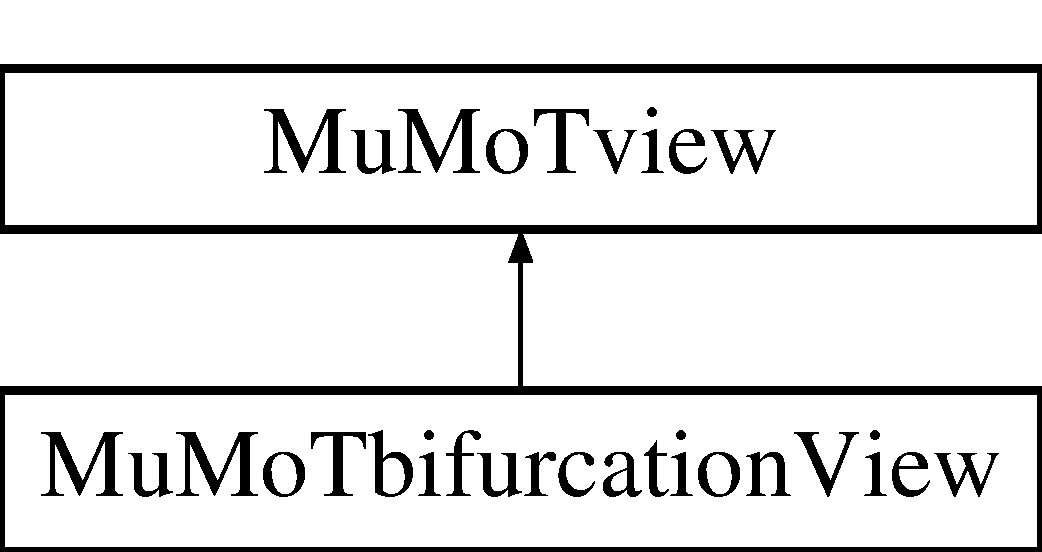
\includegraphics[height=2.000000cm]{class_mu_mo_t_1_1_mu_mo_tbifurcation_view}
\end{center}
\end{figure}
\subsection*{Public Member Functions}
\begin{DoxyCompactItemize}
\item 
def \hyperlink{class_mu_mo_t_1_1_mu_mo_tbifurcation_view_a7b55446edcef0a16d6840cd227f200b8}{\+\_\+\+\_\+init\+\_\+\+\_\+} (self, model, controller, param\+Dict, bifurcation\+Parameter, state\+Variable1, state\+Variable2, \hyperlink{class_mu_mo_t_1_1_mu_mo_tbifurcation_view_a391e34f2de441d79152a7b3d6e4c9c86}{figure}=None, params=None, kwargs)
\end{DoxyCompactItemize}
\subsection*{Static Public Attributes}
\begin{DoxyCompactItemize}
\item 
dictionary \hyperlink{class_mu_mo_t_1_1_mu_mo_tbifurcation_view_a23ca095d6146b220be161f1f73017674}{initconds} = \{state\+Variable1\+: self.\+\_\+py\+D\+Smodel.\+pars\mbox{[}str(self.\+\_\+mumot\+Model.\+\_\+system\+Size)\mbox{]} / len(self.\+\_\+mumot\+Model.\+\_\+reactants)\}
\item 
\hyperlink{class_mu_mo_t_1_1_mu_mo_tbifurcation_view_a08c7b0edb053705a8c47fe487b6f53bd}{ics}
\item 
\hyperlink{class_mu_mo_t_1_1_mu_mo_tbifurcation_view_a372cc7d4f485e77e35668d40b507d0e5}{pars}
\item 
\hyperlink{class_mu_mo_t_1_1_mu_mo_tbifurcation_view_ab74e6bf80237ddc4109968cedc58c151}{name}
\item 
\hyperlink{class_mu_mo_t_1_1_mu_mo_tbifurcation_view_a7aead736a07eaf25623ad7bfa1f0ee2d}{type}
\item 
\hyperlink{class_mu_mo_t_1_1_mu_mo_tbifurcation_view_a15cf90b3888db001a8299a477d50af98}{freepars}
\item 
\hyperlink{class_mu_mo_t_1_1_mu_mo_tbifurcation_view_aaa677c130e36435865b68ff6230a932d}{Max\+Num\+Points}
\item 
\hyperlink{class_mu_mo_t_1_1_mu_mo_tbifurcation_view_a0a7557ffe670b6a318afa8bd9851d2fc}{Max\+Step\+Size}
\begin{DoxyCompactList}\small\item\em The following 3 parameters are set after trial-\/and-\/error. \end{DoxyCompactList}\item 
\hyperlink{class_mu_mo_t_1_1_mu_mo_tbifurcation_view_a5fe506ca005e76a55ccd505a36e17fe6}{Min\+Step\+Size}
\item 
\hyperlink{class_mu_mo_t_1_1_mu_mo_tbifurcation_view_a9c25479455e9bdd389f37c4bccfefea1}{Step\+Size}
\item 
\hyperlink{class_mu_mo_t_1_1_mu_mo_tbifurcation_view_a7ff5325c1fceeebd63c3e4805a2206c8}{Loc\+Bif\+Points}
\item 
\hyperlink{class_mu_mo_t_1_1_mu_mo_tbifurcation_view_a040a7ecbcbaca807aeaec6d5c81801d5}{Save\+Eigen}
\item 
\hyperlink{class_mu_mo_t_1_1_mu_mo_tbifurcation_view_a1df8fcdacfec00fc258a3c72772c2f18}{stability}
\begin{DoxyCompactList}\small\item\em use internal plotting routines ( \end{DoxyCompactList}\item 
\hyperlink{class_mu_mo_t_1_1_mu_mo_tbifurcation_view_a643a20c0c59588a0f741a6095e2025fd}{True}
\item 
\hyperlink{class_mu_mo_t_1_1_mu_mo_tbifurcation_view_a391e34f2de441d79152a7b3d6e4c9c86}{figure}
\end{DoxyCompactItemize}
\subsection*{Private Member Functions}
\begin{DoxyCompactItemize}
\item 
def \hyperlink{class_mu_mo_t_1_1_mu_mo_tbifurcation_view_a385e5f82733060fec5122635ae6a8e67}{\+\_\+plot\+\_\+bifurcation} (self)
\item 
def \hyperlink{class_mu_mo_t_1_1_mu_mo_tbifurcation_view_a13b207330e0a4fe5bb7c3b863bbd0820}{\+\_\+replot\+\_\+bifurcation} (self)
\end{DoxyCompactItemize}
\subsection*{Static Private Attributes}
\begin{DoxyCompactItemize}
\item 
\hyperlink{class_mu_mo_t_1_1_mu_mo_tbifurcation_view_a9e9a430da6d323cc4411c070e0c7eee5}{\+\_\+py\+D\+Smodel} = None
\item 
\hyperlink{class_mu_mo_t_1_1_mu_mo_tbifurcation_view_a17d5bd0e623faea6f50fc3b7f01d0d38}{\+\_\+bifurcation\+Parameter} = None
\item 
\hyperlink{class_mu_mo_t_1_1_mu_mo_tbifurcation_view_aa14fa36730691becc6f3136899545416}{\+\_\+state\+Variable1} = None
\item 
\hyperlink{class_mu_mo_t_1_1_mu_mo_tbifurcation_view_a9d3705d1d9182e10751ff693573d6d16}{\+\_\+state\+Variable2} = None
\item 
\hyperlink{class_mu_mo_t_1_1_mu_mo_tbifurcation_view_ad2f8dc44173a16468bd9d3ab335f9b27}{\+\_\+state\+Variable3}
\begin{DoxyCompactList}\small\item\em 3-\/d bifurcation diagram ( \end{DoxyCompactList}\item 
\hyperlink{class_mu_mo_t_1_1_mu_mo_tbifurcation_view_a45f0a60363e440604d8e5b08930eb7b5}{\+\_\+py\+D\+Sode}
\item 
\hyperlink{class_mu_mo_t_1_1_mu_mo_tbifurcation_view_a797e92fe19ce2636a49bf1400a69fc49}{\+\_\+py\+D\+Scont}
\begin{DoxyCompactList}\small\item\em @todo remove magic number \end{DoxyCompactList}\item 
\hyperlink{class_mu_mo_t_1_1_mu_mo_tbifurcation_view_aa56e2cffc879be68fdec55f29334415c}{\+\_\+py\+D\+Scont\+Args}
\item 
\hyperlink{class_mu_mo_t_1_1_mu_mo_tbifurcation_view_a5feff4ca83ee97d6e09874496a4975d4}{\+\_\+plot\+Type}
\end{DoxyCompactItemize}


\subsection{Detailed Description}
bifurcation view on model 

\subsection{Constructor \& Destructor Documentation}
\mbox{\Hypertarget{class_mu_mo_t_1_1_mu_mo_tbifurcation_view_a7b55446edcef0a16d6840cd227f200b8}\label{class_mu_mo_t_1_1_mu_mo_tbifurcation_view_a7b55446edcef0a16d6840cd227f200b8}} 
\index{Mu\+Mo\+T\+::\+Mu\+Mo\+Tbifurcation\+View@{Mu\+Mo\+T\+::\+Mu\+Mo\+Tbifurcation\+View}!\+\_\+\+\_\+init\+\_\+\+\_\+@{\+\_\+\+\_\+init\+\_\+\+\_\+}}
\index{\+\_\+\+\_\+init\+\_\+\+\_\+@{\+\_\+\+\_\+init\+\_\+\+\_\+}!Mu\+Mo\+T\+::\+Mu\+Mo\+Tbifurcation\+View@{Mu\+Mo\+T\+::\+Mu\+Mo\+Tbifurcation\+View}}
\subsubsection{\texorpdfstring{\+\_\+\+\_\+init\+\_\+\+\_\+()}{\_\_init\_\_()}}
{\footnotesize\ttfamily def \+\_\+\+\_\+init\+\_\+\+\_\+ (\begin{DoxyParamCaption}\item[{}]{self,  }\item[{}]{model,  }\item[{}]{controller,  }\item[{}]{param\+Dict,  }\item[{}]{bifurcation\+Parameter,  }\item[{}]{state\+Variable1,  }\item[{}]{state\+Variable2,  }\item[{}]{figure = {\ttfamily None},  }\item[{}]{params = {\ttfamily None},  }\item[{}]{kwargs }\end{DoxyParamCaption})}



\subsection{Member Function Documentation}
\mbox{\Hypertarget{class_mu_mo_t_1_1_mu_mo_tbifurcation_view_a385e5f82733060fec5122635ae6a8e67}\label{class_mu_mo_t_1_1_mu_mo_tbifurcation_view_a385e5f82733060fec5122635ae6a8e67}} 
\index{Mu\+Mo\+T\+::\+Mu\+Mo\+Tbifurcation\+View@{Mu\+Mo\+T\+::\+Mu\+Mo\+Tbifurcation\+View}!\+\_\+plot\+\_\+bifurcation@{\+\_\+plot\+\_\+bifurcation}}
\index{\+\_\+plot\+\_\+bifurcation@{\+\_\+plot\+\_\+bifurcation}!Mu\+Mo\+T\+::\+Mu\+Mo\+Tbifurcation\+View@{Mu\+Mo\+T\+::\+Mu\+Mo\+Tbifurcation\+View}}
\subsubsection{\texorpdfstring{\+\_\+plot\+\_\+bifurcation()}{\_plot\_bifurcation()}}
{\footnotesize\ttfamily def \+\_\+plot\+\_\+bifurcation (\begin{DoxyParamCaption}\item[{}]{self }\end{DoxyParamCaption})\hspace{0.3cm}{\ttfamily [private]}}

\mbox{\Hypertarget{class_mu_mo_t_1_1_mu_mo_tbifurcation_view_a13b207330e0a4fe5bb7c3b863bbd0820}\label{class_mu_mo_t_1_1_mu_mo_tbifurcation_view_a13b207330e0a4fe5bb7c3b863bbd0820}} 
\index{Mu\+Mo\+T\+::\+Mu\+Mo\+Tbifurcation\+View@{Mu\+Mo\+T\+::\+Mu\+Mo\+Tbifurcation\+View}!\+\_\+replot\+\_\+bifurcation@{\+\_\+replot\+\_\+bifurcation}}
\index{\+\_\+replot\+\_\+bifurcation@{\+\_\+replot\+\_\+bifurcation}!Mu\+Mo\+T\+::\+Mu\+Mo\+Tbifurcation\+View@{Mu\+Mo\+T\+::\+Mu\+Mo\+Tbifurcation\+View}}
\subsubsection{\texorpdfstring{\+\_\+replot\+\_\+bifurcation()}{\_replot\_bifurcation()}}
{\footnotesize\ttfamily def \+\_\+replot\+\_\+bifurcation (\begin{DoxyParamCaption}\item[{}]{self }\end{DoxyParamCaption})\hspace{0.3cm}{\ttfamily [private]}}



\subsection{Field Documentation}
\mbox{\Hypertarget{class_mu_mo_t_1_1_mu_mo_tbifurcation_view_a17d5bd0e623faea6f50fc3b7f01d0d38}\label{class_mu_mo_t_1_1_mu_mo_tbifurcation_view_a17d5bd0e623faea6f50fc3b7f01d0d38}} 
\index{Mu\+Mo\+T\+::\+Mu\+Mo\+Tbifurcation\+View@{Mu\+Mo\+T\+::\+Mu\+Mo\+Tbifurcation\+View}!\+\_\+bifurcation\+Parameter@{\+\_\+bifurcation\+Parameter}}
\index{\+\_\+bifurcation\+Parameter@{\+\_\+bifurcation\+Parameter}!Mu\+Mo\+T\+::\+Mu\+Mo\+Tbifurcation\+View@{Mu\+Mo\+T\+::\+Mu\+Mo\+Tbifurcation\+View}}
\subsubsection{\texorpdfstring{\+\_\+bifurcation\+Parameter}{\_bifurcationParameter}}
{\footnotesize\ttfamily \+\_\+bifurcation\+Parameter = None\hspace{0.3cm}{\ttfamily [static]}, {\ttfamily [private]}}

\mbox{\Hypertarget{class_mu_mo_t_1_1_mu_mo_tbifurcation_view_a5feff4ca83ee97d6e09874496a4975d4}\label{class_mu_mo_t_1_1_mu_mo_tbifurcation_view_a5feff4ca83ee97d6e09874496a4975d4}} 
\index{Mu\+Mo\+T\+::\+Mu\+Mo\+Tbifurcation\+View@{Mu\+Mo\+T\+::\+Mu\+Mo\+Tbifurcation\+View}!\+\_\+plot\+Type@{\+\_\+plot\+Type}}
\index{\+\_\+plot\+Type@{\+\_\+plot\+Type}!Mu\+Mo\+T\+::\+Mu\+Mo\+Tbifurcation\+View@{Mu\+Mo\+T\+::\+Mu\+Mo\+Tbifurcation\+View}}
\subsubsection{\texorpdfstring{\+\_\+plot\+Type}{\_plotType}}
{\footnotesize\ttfamily \+\_\+plot\+Type\hspace{0.3cm}{\ttfamily [static]}, {\ttfamily [private]}}

\mbox{\Hypertarget{class_mu_mo_t_1_1_mu_mo_tbifurcation_view_a797e92fe19ce2636a49bf1400a69fc49}\label{class_mu_mo_t_1_1_mu_mo_tbifurcation_view_a797e92fe19ce2636a49bf1400a69fc49}} 
\index{Mu\+Mo\+T\+::\+Mu\+Mo\+Tbifurcation\+View@{Mu\+Mo\+T\+::\+Mu\+Mo\+Tbifurcation\+View}!\+\_\+py\+D\+Scont@{\+\_\+py\+D\+Scont}}
\index{\+\_\+py\+D\+Scont@{\+\_\+py\+D\+Scont}!Mu\+Mo\+T\+::\+Mu\+Mo\+Tbifurcation\+View@{Mu\+Mo\+T\+::\+Mu\+Mo\+Tbifurcation\+View}}
\subsubsection{\texorpdfstring{\+\_\+py\+D\+Scont}{\_pyDScont}}
{\footnotesize\ttfamily \+\_\+py\+D\+Scont\hspace{0.3cm}{\ttfamily [static]}, {\ttfamily [private]}}



@todo remove magic number 

\begin{DoxyRefDesc}{Todo}
\item[\hyperlink{todo__todo000046}{Todo}]\+: add to {\bfseries init}() \end{DoxyRefDesc}
\begin{DoxyRefDesc}{Todo}
\item[\hyperlink{todo__todo000047}{Todo}]remove magic number \end{DoxyRefDesc}
\mbox{\Hypertarget{class_mu_mo_t_1_1_mu_mo_tbifurcation_view_aa56e2cffc879be68fdec55f29334415c}\label{class_mu_mo_t_1_1_mu_mo_tbifurcation_view_aa56e2cffc879be68fdec55f29334415c}} 
\index{Mu\+Mo\+T\+::\+Mu\+Mo\+Tbifurcation\+View@{Mu\+Mo\+T\+::\+Mu\+Mo\+Tbifurcation\+View}!\+\_\+py\+D\+Scont\+Args@{\+\_\+py\+D\+Scont\+Args}}
\index{\+\_\+py\+D\+Scont\+Args@{\+\_\+py\+D\+Scont\+Args}!Mu\+Mo\+T\+::\+Mu\+Mo\+Tbifurcation\+View@{Mu\+Mo\+T\+::\+Mu\+Mo\+Tbifurcation\+View}}
\subsubsection{\texorpdfstring{\+\_\+py\+D\+Scont\+Args}{\_pyDScontArgs}}
{\footnotesize\ttfamily \+\_\+py\+D\+Scont\+Args\hspace{0.3cm}{\ttfamily [static]}, {\ttfamily [private]}}

\begin{DoxyRefDesc}{Todo}
\item[\hyperlink{todo__todo000040}{Todo}]\+: add self.\+\_\+py\+D\+Scont\+Args to {\bfseries init}() \end{DoxyRefDesc}
\mbox{\Hypertarget{class_mu_mo_t_1_1_mu_mo_tbifurcation_view_a9e9a430da6d323cc4411c070e0c7eee5}\label{class_mu_mo_t_1_1_mu_mo_tbifurcation_view_a9e9a430da6d323cc4411c070e0c7eee5}} 
\index{Mu\+Mo\+T\+::\+Mu\+Mo\+Tbifurcation\+View@{Mu\+Mo\+T\+::\+Mu\+Mo\+Tbifurcation\+View}!\+\_\+py\+D\+Smodel@{\+\_\+py\+D\+Smodel}}
\index{\+\_\+py\+D\+Smodel@{\+\_\+py\+D\+Smodel}!Mu\+Mo\+T\+::\+Mu\+Mo\+Tbifurcation\+View@{Mu\+Mo\+T\+::\+Mu\+Mo\+Tbifurcation\+View}}
\subsubsection{\texorpdfstring{\+\_\+py\+D\+Smodel}{\_pyDSmodel}}
{\footnotesize\ttfamily \+\_\+py\+D\+Smodel = None\hspace{0.3cm}{\ttfamily [static]}, {\ttfamily [private]}}

\mbox{\Hypertarget{class_mu_mo_t_1_1_mu_mo_tbifurcation_view_a45f0a60363e440604d8e5b08930eb7b5}\label{class_mu_mo_t_1_1_mu_mo_tbifurcation_view_a45f0a60363e440604d8e5b08930eb7b5}} 
\index{Mu\+Mo\+T\+::\+Mu\+Mo\+Tbifurcation\+View@{Mu\+Mo\+T\+::\+Mu\+Mo\+Tbifurcation\+View}!\+\_\+py\+D\+Sode@{\+\_\+py\+D\+Sode}}
\index{\+\_\+py\+D\+Sode@{\+\_\+py\+D\+Sode}!Mu\+Mo\+T\+::\+Mu\+Mo\+Tbifurcation\+View@{Mu\+Mo\+T\+::\+Mu\+Mo\+Tbifurcation\+View}}
\subsubsection{\texorpdfstring{\+\_\+py\+D\+Sode}{\_pyDSode}}
{\footnotesize\ttfamily \+\_\+py\+D\+Sode\hspace{0.3cm}{\ttfamily [static]}, {\ttfamily [private]}}

\mbox{\Hypertarget{class_mu_mo_t_1_1_mu_mo_tbifurcation_view_aa14fa36730691becc6f3136899545416}\label{class_mu_mo_t_1_1_mu_mo_tbifurcation_view_aa14fa36730691becc6f3136899545416}} 
\index{Mu\+Mo\+T\+::\+Mu\+Mo\+Tbifurcation\+View@{Mu\+Mo\+T\+::\+Mu\+Mo\+Tbifurcation\+View}!\+\_\+state\+Variable1@{\+\_\+state\+Variable1}}
\index{\+\_\+state\+Variable1@{\+\_\+state\+Variable1}!Mu\+Mo\+T\+::\+Mu\+Mo\+Tbifurcation\+View@{Mu\+Mo\+T\+::\+Mu\+Mo\+Tbifurcation\+View}}
\subsubsection{\texorpdfstring{\+\_\+state\+Variable1}{\_stateVariable1}}
{\footnotesize\ttfamily \+\_\+state\+Variable1 = None\hspace{0.3cm}{\ttfamily [static]}, {\ttfamily [private]}}

\mbox{\Hypertarget{class_mu_mo_t_1_1_mu_mo_tbifurcation_view_a9d3705d1d9182e10751ff693573d6d16}\label{class_mu_mo_t_1_1_mu_mo_tbifurcation_view_a9d3705d1d9182e10751ff693573d6d16}} 
\index{Mu\+Mo\+T\+::\+Mu\+Mo\+Tbifurcation\+View@{Mu\+Mo\+T\+::\+Mu\+Mo\+Tbifurcation\+View}!\+\_\+state\+Variable2@{\+\_\+state\+Variable2}}
\index{\+\_\+state\+Variable2@{\+\_\+state\+Variable2}!Mu\+Mo\+T\+::\+Mu\+Mo\+Tbifurcation\+View@{Mu\+Mo\+T\+::\+Mu\+Mo\+Tbifurcation\+View}}
\subsubsection{\texorpdfstring{\+\_\+state\+Variable2}{\_stateVariable2}}
{\footnotesize\ttfamily \+\_\+state\+Variable2 = None\hspace{0.3cm}{\ttfamily [static]}, {\ttfamily [private]}}

\mbox{\Hypertarget{class_mu_mo_t_1_1_mu_mo_tbifurcation_view_ad2f8dc44173a16468bd9d3ab335f9b27}\label{class_mu_mo_t_1_1_mu_mo_tbifurcation_view_ad2f8dc44173a16468bd9d3ab335f9b27}} 
\index{Mu\+Mo\+T\+::\+Mu\+Mo\+Tbifurcation\+View@{Mu\+Mo\+T\+::\+Mu\+Mo\+Tbifurcation\+View}!\+\_\+state\+Variable3@{\+\_\+state\+Variable3}}
\index{\+\_\+state\+Variable3@{\+\_\+state\+Variable3}!Mu\+Mo\+T\+::\+Mu\+Mo\+Tbifurcation\+View@{Mu\+Mo\+T\+::\+Mu\+Mo\+Tbifurcation\+View}}
\subsubsection{\texorpdfstring{\+\_\+state\+Variable3}{\_stateVariable3}}
{\footnotesize\ttfamily \+\_\+state\+Variable3\hspace{0.3cm}{\ttfamily [static]}, {\ttfamily [private]}}



3-\/d bifurcation diagram ( 

\begin{DoxyRefDesc}{Todo}
\item[\hyperlink{todo__todo000039}{Todo}]\+: currently unsupported) \end{DoxyRefDesc}
\mbox{\Hypertarget{class_mu_mo_t_1_1_mu_mo_tbifurcation_view_a391e34f2de441d79152a7b3d6e4c9c86}\label{class_mu_mo_t_1_1_mu_mo_tbifurcation_view_a391e34f2de441d79152a7b3d6e4c9c86}} 
\index{Mu\+Mo\+T\+::\+Mu\+Mo\+Tbifurcation\+View@{Mu\+Mo\+T\+::\+Mu\+Mo\+Tbifurcation\+View}!figure@{figure}}
\index{figure@{figure}!Mu\+Mo\+T\+::\+Mu\+Mo\+Tbifurcation\+View@{Mu\+Mo\+T\+::\+Mu\+Mo\+Tbifurcation\+View}}
\subsubsection{\texorpdfstring{figure}{figure}}
{\footnotesize\ttfamily figure\hspace{0.3cm}{\ttfamily [static]}}

\mbox{\Hypertarget{class_mu_mo_t_1_1_mu_mo_tbifurcation_view_a15cf90b3888db001a8299a477d50af98}\label{class_mu_mo_t_1_1_mu_mo_tbifurcation_view_a15cf90b3888db001a8299a477d50af98}} 
\index{Mu\+Mo\+T\+::\+Mu\+Mo\+Tbifurcation\+View@{Mu\+Mo\+T\+::\+Mu\+Mo\+Tbifurcation\+View}!freepars@{freepars}}
\index{freepars@{freepars}!Mu\+Mo\+T\+::\+Mu\+Mo\+Tbifurcation\+View@{Mu\+Mo\+T\+::\+Mu\+Mo\+Tbifurcation\+View}}
\subsubsection{\texorpdfstring{freepars}{freepars}}
{\footnotesize\ttfamily freepars\hspace{0.3cm}{\ttfamily [static]}}

\mbox{\Hypertarget{class_mu_mo_t_1_1_mu_mo_tbifurcation_view_a08c7b0edb053705a8c47fe487b6f53bd}\label{class_mu_mo_t_1_1_mu_mo_tbifurcation_view_a08c7b0edb053705a8c47fe487b6f53bd}} 
\index{Mu\+Mo\+T\+::\+Mu\+Mo\+Tbifurcation\+View@{Mu\+Mo\+T\+::\+Mu\+Mo\+Tbifurcation\+View}!ics@{ics}}
\index{ics@{ics}!Mu\+Mo\+T\+::\+Mu\+Mo\+Tbifurcation\+View@{Mu\+Mo\+T\+::\+Mu\+Mo\+Tbifurcation\+View}}
\subsubsection{\texorpdfstring{ics}{ics}}
{\footnotesize\ttfamily ics\hspace{0.3cm}{\ttfamily [static]}}

\mbox{\Hypertarget{class_mu_mo_t_1_1_mu_mo_tbifurcation_view_a23ca095d6146b220be161f1f73017674}\label{class_mu_mo_t_1_1_mu_mo_tbifurcation_view_a23ca095d6146b220be161f1f73017674}} 
\index{Mu\+Mo\+T\+::\+Mu\+Mo\+Tbifurcation\+View@{Mu\+Mo\+T\+::\+Mu\+Mo\+Tbifurcation\+View}!initconds@{initconds}}
\index{initconds@{initconds}!Mu\+Mo\+T\+::\+Mu\+Mo\+Tbifurcation\+View@{Mu\+Mo\+T\+::\+Mu\+Mo\+Tbifurcation\+View}}
\subsubsection{\texorpdfstring{initconds}{initconds}}
{\footnotesize\ttfamily dictionary initconds = \{state\+Variable1\+: self.\+\_\+py\+D\+Smodel.\+pars\mbox{[}str(self.\+\_\+mumot\+Model.\+\_\+system\+Size)\mbox{]} / len(self.\+\_\+mumot\+Model.\+\_\+reactants)\}\hspace{0.3cm}{\ttfamily [static]}}

\mbox{\Hypertarget{class_mu_mo_t_1_1_mu_mo_tbifurcation_view_a7ff5325c1fceeebd63c3e4805a2206c8}\label{class_mu_mo_t_1_1_mu_mo_tbifurcation_view_a7ff5325c1fceeebd63c3e4805a2206c8}} 
\index{Mu\+Mo\+T\+::\+Mu\+Mo\+Tbifurcation\+View@{Mu\+Mo\+T\+::\+Mu\+Mo\+Tbifurcation\+View}!Loc\+Bif\+Points@{Loc\+Bif\+Points}}
\index{Loc\+Bif\+Points@{Loc\+Bif\+Points}!Mu\+Mo\+T\+::\+Mu\+Mo\+Tbifurcation\+View@{Mu\+Mo\+T\+::\+Mu\+Mo\+Tbifurcation\+View}}
\subsubsection{\texorpdfstring{Loc\+Bif\+Points}{LocBifPoints}}
{\footnotesize\ttfamily Loc\+Bif\+Points\hspace{0.3cm}{\ttfamily [static]}}

\mbox{\Hypertarget{class_mu_mo_t_1_1_mu_mo_tbifurcation_view_aaa677c130e36435865b68ff6230a932d}\label{class_mu_mo_t_1_1_mu_mo_tbifurcation_view_aaa677c130e36435865b68ff6230a932d}} 
\index{Mu\+Mo\+T\+::\+Mu\+Mo\+Tbifurcation\+View@{Mu\+Mo\+T\+::\+Mu\+Mo\+Tbifurcation\+View}!Max\+Num\+Points@{Max\+Num\+Points}}
\index{Max\+Num\+Points@{Max\+Num\+Points}!Mu\+Mo\+T\+::\+Mu\+Mo\+Tbifurcation\+View@{Mu\+Mo\+T\+::\+Mu\+Mo\+Tbifurcation\+View}}
\subsubsection{\texorpdfstring{Max\+Num\+Points}{MaxNumPoints}}
{\footnotesize\ttfamily Max\+Num\+Points\hspace{0.3cm}{\ttfamily [static]}}

\mbox{\Hypertarget{class_mu_mo_t_1_1_mu_mo_tbifurcation_view_a0a7557ffe670b6a318afa8bd9851d2fc}\label{class_mu_mo_t_1_1_mu_mo_tbifurcation_view_a0a7557ffe670b6a318afa8bd9851d2fc}} 
\index{Mu\+Mo\+T\+::\+Mu\+Mo\+Tbifurcation\+View@{Mu\+Mo\+T\+::\+Mu\+Mo\+Tbifurcation\+View}!Max\+Step\+Size@{Max\+Step\+Size}}
\index{Max\+Step\+Size@{Max\+Step\+Size}!Mu\+Mo\+T\+::\+Mu\+Mo\+Tbifurcation\+View@{Mu\+Mo\+T\+::\+Mu\+Mo\+Tbifurcation\+View}}
\subsubsection{\texorpdfstring{Max\+Step\+Size}{MaxStepSize}}
{\footnotesize\ttfamily Max\+Step\+Size\hspace{0.3cm}{\ttfamily [static]}}



The following 3 parameters are set after trial-\/and-\/error. 

\begin{DoxyRefDesc}{Todo}
\item[\hyperlink{todo__todo000041}{Todo}]\+: how to automate this? \end{DoxyRefDesc}
\mbox{\Hypertarget{class_mu_mo_t_1_1_mu_mo_tbifurcation_view_a5fe506ca005e76a55ccd505a36e17fe6}\label{class_mu_mo_t_1_1_mu_mo_tbifurcation_view_a5fe506ca005e76a55ccd505a36e17fe6}} 
\index{Mu\+Mo\+T\+::\+Mu\+Mo\+Tbifurcation\+View@{Mu\+Mo\+T\+::\+Mu\+Mo\+Tbifurcation\+View}!Min\+Step\+Size@{Min\+Step\+Size}}
\index{Min\+Step\+Size@{Min\+Step\+Size}!Mu\+Mo\+T\+::\+Mu\+Mo\+Tbifurcation\+View@{Mu\+Mo\+T\+::\+Mu\+Mo\+Tbifurcation\+View}}
\subsubsection{\texorpdfstring{Min\+Step\+Size}{MinStepSize}}
{\footnotesize\ttfamily Min\+Step\+Size\hspace{0.3cm}{\ttfamily [static]}}

\mbox{\Hypertarget{class_mu_mo_t_1_1_mu_mo_tbifurcation_view_ab74e6bf80237ddc4109968cedc58c151}\label{class_mu_mo_t_1_1_mu_mo_tbifurcation_view_ab74e6bf80237ddc4109968cedc58c151}} 
\index{Mu\+Mo\+T\+::\+Mu\+Mo\+Tbifurcation\+View@{Mu\+Mo\+T\+::\+Mu\+Mo\+Tbifurcation\+View}!name@{name}}
\index{name@{name}!Mu\+Mo\+T\+::\+Mu\+Mo\+Tbifurcation\+View@{Mu\+Mo\+T\+::\+Mu\+Mo\+Tbifurcation\+View}}
\subsubsection{\texorpdfstring{name}{name}}
{\footnotesize\ttfamily name\hspace{0.3cm}{\ttfamily [static]}}

\mbox{\Hypertarget{class_mu_mo_t_1_1_mu_mo_tbifurcation_view_a372cc7d4f485e77e35668d40b507d0e5}\label{class_mu_mo_t_1_1_mu_mo_tbifurcation_view_a372cc7d4f485e77e35668d40b507d0e5}} 
\index{Mu\+Mo\+T\+::\+Mu\+Mo\+Tbifurcation\+View@{Mu\+Mo\+T\+::\+Mu\+Mo\+Tbifurcation\+View}!pars@{pars}}
\index{pars@{pars}!Mu\+Mo\+T\+::\+Mu\+Mo\+Tbifurcation\+View@{Mu\+Mo\+T\+::\+Mu\+Mo\+Tbifurcation\+View}}
\subsubsection{\texorpdfstring{pars}{pars}}
{\footnotesize\ttfamily pars\hspace{0.3cm}{\ttfamily [static]}}

\mbox{\Hypertarget{class_mu_mo_t_1_1_mu_mo_tbifurcation_view_a040a7ecbcbaca807aeaec6d5c81801d5}\label{class_mu_mo_t_1_1_mu_mo_tbifurcation_view_a040a7ecbcbaca807aeaec6d5c81801d5}} 
\index{Mu\+Mo\+T\+::\+Mu\+Mo\+Tbifurcation\+View@{Mu\+Mo\+T\+::\+Mu\+Mo\+Tbifurcation\+View}!Save\+Eigen@{Save\+Eigen}}
\index{Save\+Eigen@{Save\+Eigen}!Mu\+Mo\+T\+::\+Mu\+Mo\+Tbifurcation\+View@{Mu\+Mo\+T\+::\+Mu\+Mo\+Tbifurcation\+View}}
\subsubsection{\texorpdfstring{Save\+Eigen}{SaveEigen}}
{\footnotesize\ttfamily Save\+Eigen\hspace{0.3cm}{\ttfamily [static]}}

\begin{DoxyRefDesc}{Todo}
\item[\hyperlink{todo__todo000042}{Todo}]W\+AS \textquotesingle{}LP\textquotesingle{} (detect limit points / saddle-\/node bifurcations) \end{DoxyRefDesc}
\mbox{\Hypertarget{class_mu_mo_t_1_1_mu_mo_tbifurcation_view_a1df8fcdacfec00fc258a3c72772c2f18}\label{class_mu_mo_t_1_1_mu_mo_tbifurcation_view_a1df8fcdacfec00fc258a3c72772c2f18}} 
\index{Mu\+Mo\+T\+::\+Mu\+Mo\+Tbifurcation\+View@{Mu\+Mo\+T\+::\+Mu\+Mo\+Tbifurcation\+View}!stability@{stability}}
\index{stability@{stability}!Mu\+Mo\+T\+::\+Mu\+Mo\+Tbifurcation\+View@{Mu\+Mo\+T\+::\+Mu\+Mo\+Tbifurcation\+View}}
\subsubsection{\texorpdfstring{stability}{stability}}
{\footnotesize\ttfamily stability\hspace{0.3cm}{\ttfamily [static]}}



use internal plotting routines ( 

\begin{DoxyRefDesc}{Todo}
\item[\hyperlink{todo__todo000043}{Todo}]\+: not yet supported) \end{DoxyRefDesc}
\mbox{\Hypertarget{class_mu_mo_t_1_1_mu_mo_tbifurcation_view_a9c25479455e9bdd389f37c4bccfefea1}\label{class_mu_mo_t_1_1_mu_mo_tbifurcation_view_a9c25479455e9bdd389f37c4bccfefea1}} 
\index{Mu\+Mo\+T\+::\+Mu\+Mo\+Tbifurcation\+View@{Mu\+Mo\+T\+::\+Mu\+Mo\+Tbifurcation\+View}!Step\+Size@{Step\+Size}}
\index{Step\+Size@{Step\+Size}!Mu\+Mo\+T\+::\+Mu\+Mo\+Tbifurcation\+View@{Mu\+Mo\+T\+::\+Mu\+Mo\+Tbifurcation\+View}}
\subsubsection{\texorpdfstring{Step\+Size}{StepSize}}
{\footnotesize\ttfamily Step\+Size\hspace{0.3cm}{\ttfamily [static]}}

\mbox{\Hypertarget{class_mu_mo_t_1_1_mu_mo_tbifurcation_view_a643a20c0c59588a0f741a6095e2025fd}\label{class_mu_mo_t_1_1_mu_mo_tbifurcation_view_a643a20c0c59588a0f741a6095e2025fd}} 
\index{Mu\+Mo\+T\+::\+Mu\+Mo\+Tbifurcation\+View@{Mu\+Mo\+T\+::\+Mu\+Mo\+Tbifurcation\+View}!True@{True}}
\index{True@{True}!Mu\+Mo\+T\+::\+Mu\+Mo\+Tbifurcation\+View@{Mu\+Mo\+T\+::\+Mu\+Mo\+Tbifurcation\+View}}
\subsubsection{\texorpdfstring{True}{True}}
{\footnotesize\ttfamily True\hspace{0.3cm}{\ttfamily [static]}}

\mbox{\Hypertarget{class_mu_mo_t_1_1_mu_mo_tbifurcation_view_a7aead736a07eaf25623ad7bfa1f0ee2d}\label{class_mu_mo_t_1_1_mu_mo_tbifurcation_view_a7aead736a07eaf25623ad7bfa1f0ee2d}} 
\index{Mu\+Mo\+T\+::\+Mu\+Mo\+Tbifurcation\+View@{Mu\+Mo\+T\+::\+Mu\+Mo\+Tbifurcation\+View}!type@{type}}
\index{type@{type}!Mu\+Mo\+T\+::\+Mu\+Mo\+Tbifurcation\+View@{Mu\+Mo\+T\+::\+Mu\+Mo\+Tbifurcation\+View}}
\subsubsection{\texorpdfstring{type}{type}}
{\footnotesize\ttfamily type\hspace{0.3cm}{\ttfamily [static]}}



The documentation for this class was generated from the following file\+:\begin{DoxyCompactItemize}
\item 
\hyperlink{_mu_mo_t_8py}{Mu\+Mo\+T.\+py}\end{DoxyCompactItemize}

\hypertarget{class_mu_mo_t_1_1_mu_mo_tcontroller}{}\section{Mu\+Mo\+Tcontroller Class Reference}
\label{class_mu_mo_t_1_1_mu_mo_tcontroller}\index{Mu\+Mo\+Tcontroller@{Mu\+Mo\+Tcontroller}}


class describing a controller for a model view  


Inheritance diagram for Mu\+Mo\+Tcontroller\+:\begin{figure}[H]
\begin{center}
\leavevmode
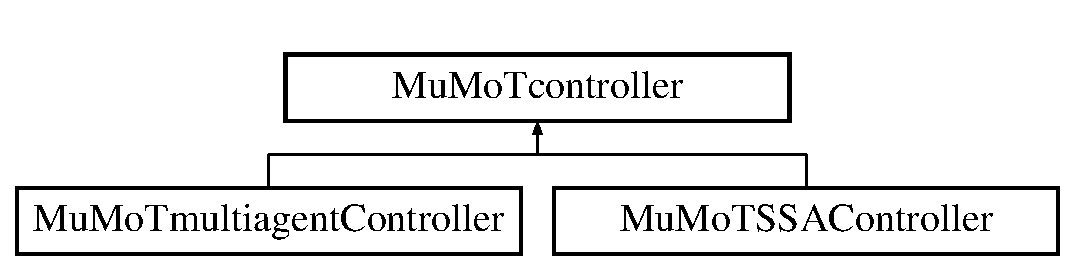
\includegraphics[height=2.000000cm]{class_mu_mo_t_1_1_mu_mo_tcontroller}
\end{center}
\end{figure}
\subsection*{Public Member Functions}
\begin{DoxyCompactItemize}
\item 
def \hyperlink{class_mu_mo_t_1_1_mu_mo_tcontroller_a73251532d0348adaeafe8a178cfc6a73}{\+\_\+\+\_\+init\+\_\+\+\_\+} (self, param\+Values, param\+Names, param\+Label\+Dict, continuous\+Replot)
\item 
def \hyperlink{class_mu_mo_t_1_1_mu_mo_tcontroller_aafc1e69cab41071217fe6676a8089249}{set\+Replot\+Function} (self, replot\+Function)
\item 
def \hyperlink{class_mu_mo_t_1_1_mu_mo_tcontroller_a40e22e664ecb6e379377ee1cea60073c}{set\+View} (self, view)
\item 
def \hyperlink{class_mu_mo_t_1_1_mu_mo_tcontroller_aca4d648d909f4722c7e07197675500bb}{show\+Logs} (self)
\item 
def \hyperlink{class_mu_mo_t_1_1_mu_mo_tcontroller_aa74bfc216071ff6b768c7a584917bfc6}{multirun} (self, iterations, random\+Seeds=\char`\"{}Auto\char`\"{}, plot\+Type=\char`\"{}evo\char`\"{}, download\+Data=False)
\end{DoxyCompactItemize}
\subsection*{Private Member Functions}
\begin{DoxyCompactItemize}
\item 
def \hyperlink{class_mu_mo_t_1_1_mu_mo_tcontroller_add4eacb8e812feeca1d4b2538e3bd6e0}{\+\_\+update\+\_\+params\+\_\+from\+\_\+widgets} (self)
\item 
def \hyperlink{class_mu_mo_t_1_1_mu_mo_tcontroller_ab703aa8fe14c83d5f12fa82d4e2c42d9}{\+\_\+download\+File} (self, data\+\_\+to\+\_\+download)
\end{DoxyCompactItemize}
\subsection*{Static Private Attributes}
\begin{DoxyCompactItemize}
\item 
\hyperlink{class_mu_mo_t_1_1_mu_mo_tcontroller_a27dd8543b5188cdfe40f622d267fe2c5}{\+\_\+view} = None
\item 
\hyperlink{class_mu_mo_t_1_1_mu_mo_tcontroller_a04608181fa27d9aad4983d3694f7ab17}{\+\_\+param\+Values} = None
\item 
\hyperlink{class_mu_mo_t_1_1_mu_mo_tcontroller_ac7734326ac8dbbf9bd0d2c9838633195}{\+\_\+param\+Names} = None
\item 
\hyperlink{class_mu_mo_t_1_1_mu_mo_tcontroller_a13bcda33e0e971cf4ad2710945226add}{\+\_\+param\+Label\+Dict} = None
\item 
\hyperlink{class_mu_mo_t_1_1_mu_mo_tcontroller_a397d0ee37a222317a1bab7deb1270a13}{\+\_\+widgets} = None
\item 
\hyperlink{class_mu_mo_t_1_1_mu_mo_tcontroller_a76e960ae74fc597cd22f7132507eaa20}{\+\_\+widget\+Dict} = None
\item 
\hyperlink{class_mu_mo_t_1_1_mu_mo_tcontroller_afb9cc1f1f0c08393b454f526842425cc}{\+\_\+error\+Message} = None
\item 
\hyperlink{class_mu_mo_t_1_1_mu_mo_tcontroller_a018864aa22d2adb0d3958fb0adbce8e2}{\+\_\+progress\+Bar} = None
\begin{DoxyCompactList}\small\item\em progress bar \end{DoxyCompactList}\item 
\hyperlink{class_mu_mo_t_1_1_mu_mo_tcontroller_a1da52cde6b2b94a1005eaa6898d2f8c5}{\+\_\+progress\+Bar\+\_\+multi} = None
\end{DoxyCompactItemize}


\subsection{Detailed Description}
class describing a controller for a model view 

\subsection{Constructor \& Destructor Documentation}
\mbox{\Hypertarget{class_mu_mo_t_1_1_mu_mo_tcontroller_a73251532d0348adaeafe8a178cfc6a73}\label{class_mu_mo_t_1_1_mu_mo_tcontroller_a73251532d0348adaeafe8a178cfc6a73}} 
\index{Mu\+Mo\+T\+::\+Mu\+Mo\+Tcontroller@{Mu\+Mo\+T\+::\+Mu\+Mo\+Tcontroller}!\+\_\+\+\_\+init\+\_\+\+\_\+@{\+\_\+\+\_\+init\+\_\+\+\_\+}}
\index{\+\_\+\+\_\+init\+\_\+\+\_\+@{\+\_\+\+\_\+init\+\_\+\+\_\+}!Mu\+Mo\+T\+::\+Mu\+Mo\+Tcontroller@{Mu\+Mo\+T\+::\+Mu\+Mo\+Tcontroller}}
\subsubsection{\texorpdfstring{\+\_\+\+\_\+init\+\_\+\+\_\+()}{\_\_init\_\_()}}
{\footnotesize\ttfamily def \+\_\+\+\_\+init\+\_\+\+\_\+ (\begin{DoxyParamCaption}\item[{}]{self,  }\item[{}]{param\+Values,  }\item[{}]{param\+Names,  }\item[{}]{param\+Label\+Dict,  }\item[{}]{continuous\+Replot }\end{DoxyParamCaption})}



\subsection{Member Function Documentation}
\mbox{\Hypertarget{class_mu_mo_t_1_1_mu_mo_tcontroller_ab703aa8fe14c83d5f12fa82d4e2c42d9}\label{class_mu_mo_t_1_1_mu_mo_tcontroller_ab703aa8fe14c83d5f12fa82d4e2c42d9}} 
\index{Mu\+Mo\+T\+::\+Mu\+Mo\+Tcontroller@{Mu\+Mo\+T\+::\+Mu\+Mo\+Tcontroller}!\+\_\+download\+File@{\+\_\+download\+File}}
\index{\+\_\+download\+File@{\+\_\+download\+File}!Mu\+Mo\+T\+::\+Mu\+Mo\+Tcontroller@{Mu\+Mo\+T\+::\+Mu\+Mo\+Tcontroller}}
\subsubsection{\texorpdfstring{\+\_\+download\+File()}{\_downloadFile()}}
{\footnotesize\ttfamily def \+\_\+download\+File (\begin{DoxyParamCaption}\item[{}]{self,  }\item[{}]{data\+\_\+to\+\_\+download }\end{DoxyParamCaption})\hspace{0.3cm}{\ttfamily [private]}}

\mbox{\Hypertarget{class_mu_mo_t_1_1_mu_mo_tcontroller_add4eacb8e812feeca1d4b2538e3bd6e0}\label{class_mu_mo_t_1_1_mu_mo_tcontroller_add4eacb8e812feeca1d4b2538e3bd6e0}} 
\index{Mu\+Mo\+T\+::\+Mu\+Mo\+Tcontroller@{Mu\+Mo\+T\+::\+Mu\+Mo\+Tcontroller}!\+\_\+update\+\_\+params\+\_\+from\+\_\+widgets@{\+\_\+update\+\_\+params\+\_\+from\+\_\+widgets}}
\index{\+\_\+update\+\_\+params\+\_\+from\+\_\+widgets@{\+\_\+update\+\_\+params\+\_\+from\+\_\+widgets}!Mu\+Mo\+T\+::\+Mu\+Mo\+Tcontroller@{Mu\+Mo\+T\+::\+Mu\+Mo\+Tcontroller}}
\subsubsection{\texorpdfstring{\+\_\+update\+\_\+params\+\_\+from\+\_\+widgets()}{\_update\_params\_from\_widgets()}}
{\footnotesize\ttfamily def \+\_\+update\+\_\+params\+\_\+from\+\_\+widgets (\begin{DoxyParamCaption}\item[{}]{self }\end{DoxyParamCaption})\hspace{0.3cm}{\ttfamily [private]}}

\mbox{\Hypertarget{class_mu_mo_t_1_1_mu_mo_tcontroller_aa74bfc216071ff6b768c7a584917bfc6}\label{class_mu_mo_t_1_1_mu_mo_tcontroller_aa74bfc216071ff6b768c7a584917bfc6}} 
\index{Mu\+Mo\+T\+::\+Mu\+Mo\+Tcontroller@{Mu\+Mo\+T\+::\+Mu\+Mo\+Tcontroller}!multirun@{multirun}}
\index{multirun@{multirun}!Mu\+Mo\+T\+::\+Mu\+Mo\+Tcontroller@{Mu\+Mo\+T\+::\+Mu\+Mo\+Tcontroller}}
\subsubsection{\texorpdfstring{multirun()}{multirun()}}
{\footnotesize\ttfamily def multirun (\begin{DoxyParamCaption}\item[{}]{self,  }\item[{}]{iterations,  }\item[{}]{random\+Seeds = {\ttfamily \char`\"{}Auto\char`\"{}},  }\item[{}]{plot\+Type = {\ttfamily \char`\"{}evo\char`\"{}},  }\item[{}]{download\+Data = {\ttfamily False} }\end{DoxyParamCaption})}

\mbox{\Hypertarget{class_mu_mo_t_1_1_mu_mo_tcontroller_aafc1e69cab41071217fe6676a8089249}\label{class_mu_mo_t_1_1_mu_mo_tcontroller_aafc1e69cab41071217fe6676a8089249}} 
\index{Mu\+Mo\+T\+::\+Mu\+Mo\+Tcontroller@{Mu\+Mo\+T\+::\+Mu\+Mo\+Tcontroller}!set\+Replot\+Function@{set\+Replot\+Function}}
\index{set\+Replot\+Function@{set\+Replot\+Function}!Mu\+Mo\+T\+::\+Mu\+Mo\+Tcontroller@{Mu\+Mo\+T\+::\+Mu\+Mo\+Tcontroller}}
\subsubsection{\texorpdfstring{set\+Replot\+Function()}{setReplotFunction()}}
{\footnotesize\ttfamily def set\+Replot\+Function (\begin{DoxyParamCaption}\item[{}]{self,  }\item[{}]{replot\+Function }\end{DoxyParamCaption})}

\mbox{\Hypertarget{class_mu_mo_t_1_1_mu_mo_tcontroller_a40e22e664ecb6e379377ee1cea60073c}\label{class_mu_mo_t_1_1_mu_mo_tcontroller_a40e22e664ecb6e379377ee1cea60073c}} 
\index{Mu\+Mo\+T\+::\+Mu\+Mo\+Tcontroller@{Mu\+Mo\+T\+::\+Mu\+Mo\+Tcontroller}!set\+View@{set\+View}}
\index{set\+View@{set\+View}!Mu\+Mo\+T\+::\+Mu\+Mo\+Tcontroller@{Mu\+Mo\+T\+::\+Mu\+Mo\+Tcontroller}}
\subsubsection{\texorpdfstring{set\+View()}{setView()}}
{\footnotesize\ttfamily def set\+View (\begin{DoxyParamCaption}\item[{}]{self,  }\item[{}]{view }\end{DoxyParamCaption})}

\mbox{\Hypertarget{class_mu_mo_t_1_1_mu_mo_tcontroller_aca4d648d909f4722c7e07197675500bb}\label{class_mu_mo_t_1_1_mu_mo_tcontroller_aca4d648d909f4722c7e07197675500bb}} 
\index{Mu\+Mo\+T\+::\+Mu\+Mo\+Tcontroller@{Mu\+Mo\+T\+::\+Mu\+Mo\+Tcontroller}!show\+Logs@{show\+Logs}}
\index{show\+Logs@{show\+Logs}!Mu\+Mo\+T\+::\+Mu\+Mo\+Tcontroller@{Mu\+Mo\+T\+::\+Mu\+Mo\+Tcontroller}}
\subsubsection{\texorpdfstring{show\+Logs()}{showLogs()}}
{\footnotesize\ttfamily def show\+Logs (\begin{DoxyParamCaption}\item[{}]{self }\end{DoxyParamCaption})}



\subsection{Field Documentation}
\mbox{\Hypertarget{class_mu_mo_t_1_1_mu_mo_tcontroller_afb9cc1f1f0c08393b454f526842425cc}\label{class_mu_mo_t_1_1_mu_mo_tcontroller_afb9cc1f1f0c08393b454f526842425cc}} 
\index{Mu\+Mo\+T\+::\+Mu\+Mo\+Tcontroller@{Mu\+Mo\+T\+::\+Mu\+Mo\+Tcontroller}!\+\_\+error\+Message@{\+\_\+error\+Message}}
\index{\+\_\+error\+Message@{\+\_\+error\+Message}!Mu\+Mo\+T\+::\+Mu\+Mo\+Tcontroller@{Mu\+Mo\+T\+::\+Mu\+Mo\+Tcontroller}}
\subsubsection{\texorpdfstring{\+\_\+error\+Message}{\_errorMessage}}
{\footnotesize\ttfamily \+\_\+error\+Message = None\hspace{0.3cm}{\ttfamily [static]}, {\ttfamily [private]}}

\mbox{\Hypertarget{class_mu_mo_t_1_1_mu_mo_tcontroller_a13bcda33e0e971cf4ad2710945226add}\label{class_mu_mo_t_1_1_mu_mo_tcontroller_a13bcda33e0e971cf4ad2710945226add}} 
\index{Mu\+Mo\+T\+::\+Mu\+Mo\+Tcontroller@{Mu\+Mo\+T\+::\+Mu\+Mo\+Tcontroller}!\+\_\+param\+Label\+Dict@{\+\_\+param\+Label\+Dict}}
\index{\+\_\+param\+Label\+Dict@{\+\_\+param\+Label\+Dict}!Mu\+Mo\+T\+::\+Mu\+Mo\+Tcontroller@{Mu\+Mo\+T\+::\+Mu\+Mo\+Tcontroller}}
\subsubsection{\texorpdfstring{\+\_\+param\+Label\+Dict}{\_paramLabelDict}}
{\footnotesize\ttfamily \+\_\+param\+Label\+Dict = None\hspace{0.3cm}{\ttfamily [static]}, {\ttfamily [private]}}

\mbox{\Hypertarget{class_mu_mo_t_1_1_mu_mo_tcontroller_ac7734326ac8dbbf9bd0d2c9838633195}\label{class_mu_mo_t_1_1_mu_mo_tcontroller_ac7734326ac8dbbf9bd0d2c9838633195}} 
\index{Mu\+Mo\+T\+::\+Mu\+Mo\+Tcontroller@{Mu\+Mo\+T\+::\+Mu\+Mo\+Tcontroller}!\+\_\+param\+Names@{\+\_\+param\+Names}}
\index{\+\_\+param\+Names@{\+\_\+param\+Names}!Mu\+Mo\+T\+::\+Mu\+Mo\+Tcontroller@{Mu\+Mo\+T\+::\+Mu\+Mo\+Tcontroller}}
\subsubsection{\texorpdfstring{\+\_\+param\+Names}{\_paramNames}}
{\footnotesize\ttfamily \+\_\+param\+Names = None\hspace{0.3cm}{\ttfamily [static]}, {\ttfamily [private]}}

\mbox{\Hypertarget{class_mu_mo_t_1_1_mu_mo_tcontroller_a04608181fa27d9aad4983d3694f7ab17}\label{class_mu_mo_t_1_1_mu_mo_tcontroller_a04608181fa27d9aad4983d3694f7ab17}} 
\index{Mu\+Mo\+T\+::\+Mu\+Mo\+Tcontroller@{Mu\+Mo\+T\+::\+Mu\+Mo\+Tcontroller}!\+\_\+param\+Values@{\+\_\+param\+Values}}
\index{\+\_\+param\+Values@{\+\_\+param\+Values}!Mu\+Mo\+T\+::\+Mu\+Mo\+Tcontroller@{Mu\+Mo\+T\+::\+Mu\+Mo\+Tcontroller}}
\subsubsection{\texorpdfstring{\+\_\+param\+Values}{\_paramValues}}
{\footnotesize\ttfamily \+\_\+param\+Values = None\hspace{0.3cm}{\ttfamily [static]}, {\ttfamily [private]}}

\mbox{\Hypertarget{class_mu_mo_t_1_1_mu_mo_tcontroller_a018864aa22d2adb0d3958fb0adbce8e2}\label{class_mu_mo_t_1_1_mu_mo_tcontroller_a018864aa22d2adb0d3958fb0adbce8e2}} 
\index{Mu\+Mo\+T\+::\+Mu\+Mo\+Tcontroller@{Mu\+Mo\+T\+::\+Mu\+Mo\+Tcontroller}!\+\_\+progress\+Bar@{\+\_\+progress\+Bar}}
\index{\+\_\+progress\+Bar@{\+\_\+progress\+Bar}!Mu\+Mo\+T\+::\+Mu\+Mo\+Tcontroller@{Mu\+Mo\+T\+::\+Mu\+Mo\+Tcontroller}}
\subsubsection{\texorpdfstring{\+\_\+progress\+Bar}{\_progressBar}}
{\footnotesize\ttfamily \+\_\+progress\+Bar = None\hspace{0.3cm}{\ttfamily [static]}, {\ttfamily [private]}}



progress bar 

\begin{DoxyRefDesc}{Todo}
\item[\hyperlink{todo__todo000018}{Todo}]\+: is this best put in base class when it is not always used? \end{DoxyRefDesc}
\mbox{\Hypertarget{class_mu_mo_t_1_1_mu_mo_tcontroller_a1da52cde6b2b94a1005eaa6898d2f8c5}\label{class_mu_mo_t_1_1_mu_mo_tcontroller_a1da52cde6b2b94a1005eaa6898d2f8c5}} 
\index{Mu\+Mo\+T\+::\+Mu\+Mo\+Tcontroller@{Mu\+Mo\+T\+::\+Mu\+Mo\+Tcontroller}!\+\_\+progress\+Bar\+\_\+multi@{\+\_\+progress\+Bar\+\_\+multi}}
\index{\+\_\+progress\+Bar\+\_\+multi@{\+\_\+progress\+Bar\+\_\+multi}!Mu\+Mo\+T\+::\+Mu\+Mo\+Tcontroller@{Mu\+Mo\+T\+::\+Mu\+Mo\+Tcontroller}}
\subsubsection{\texorpdfstring{\+\_\+progress\+Bar\+\_\+multi}{\_progressBar\_multi}}
{\footnotesize\ttfamily \+\_\+progress\+Bar\+\_\+multi = None\hspace{0.3cm}{\ttfamily [static]}, {\ttfamily [private]}}

\mbox{\Hypertarget{class_mu_mo_t_1_1_mu_mo_tcontroller_a27dd8543b5188cdfe40f622d267fe2c5}\label{class_mu_mo_t_1_1_mu_mo_tcontroller_a27dd8543b5188cdfe40f622d267fe2c5}} 
\index{Mu\+Mo\+T\+::\+Mu\+Mo\+Tcontroller@{Mu\+Mo\+T\+::\+Mu\+Mo\+Tcontroller}!\+\_\+view@{\+\_\+view}}
\index{\+\_\+view@{\+\_\+view}!Mu\+Mo\+T\+::\+Mu\+Mo\+Tcontroller@{Mu\+Mo\+T\+::\+Mu\+Mo\+Tcontroller}}
\subsubsection{\texorpdfstring{\+\_\+view}{\_view}}
{\footnotesize\ttfamily \+\_\+view = None\hspace{0.3cm}{\ttfamily [static]}, {\ttfamily [private]}}

\mbox{\Hypertarget{class_mu_mo_t_1_1_mu_mo_tcontroller_a76e960ae74fc597cd22f7132507eaa20}\label{class_mu_mo_t_1_1_mu_mo_tcontroller_a76e960ae74fc597cd22f7132507eaa20}} 
\index{Mu\+Mo\+T\+::\+Mu\+Mo\+Tcontroller@{Mu\+Mo\+T\+::\+Mu\+Mo\+Tcontroller}!\+\_\+widget\+Dict@{\+\_\+widget\+Dict}}
\index{\+\_\+widget\+Dict@{\+\_\+widget\+Dict}!Mu\+Mo\+T\+::\+Mu\+Mo\+Tcontroller@{Mu\+Mo\+T\+::\+Mu\+Mo\+Tcontroller}}
\subsubsection{\texorpdfstring{\+\_\+widget\+Dict}{\_widgetDict}}
{\footnotesize\ttfamily \+\_\+widget\+Dict = None\hspace{0.3cm}{\ttfamily [static]}, {\ttfamily [private]}}

\mbox{\Hypertarget{class_mu_mo_t_1_1_mu_mo_tcontroller_a397d0ee37a222317a1bab7deb1270a13}\label{class_mu_mo_t_1_1_mu_mo_tcontroller_a397d0ee37a222317a1bab7deb1270a13}} 
\index{Mu\+Mo\+T\+::\+Mu\+Mo\+Tcontroller@{Mu\+Mo\+T\+::\+Mu\+Mo\+Tcontroller}!\+\_\+widgets@{\+\_\+widgets}}
\index{\+\_\+widgets@{\+\_\+widgets}!Mu\+Mo\+T\+::\+Mu\+Mo\+Tcontroller@{Mu\+Mo\+T\+::\+Mu\+Mo\+Tcontroller}}
\subsubsection{\texorpdfstring{\+\_\+widgets}{\_widgets}}
{\footnotesize\ttfamily \+\_\+widgets = None\hspace{0.3cm}{\ttfamily [static]}, {\ttfamily [private]}}



The documentation for this class was generated from the following file\+:\begin{DoxyCompactItemize}
\item 
\hyperlink{_mu_mo_t_8py}{Mu\+Mo\+T.\+py}\end{DoxyCompactItemize}

\hypertarget{class_mu_mo_t_1_1_mu_mo_tdefault}{}\section{Mu\+Mo\+Tdefault Class Reference}
\label{class_mu_mo_t_1_1_mu_mo_tdefault}\index{Mu\+Mo\+Tdefault@{Mu\+Mo\+Tdefault}}
\subsection*{Static Public Member Functions}
\begin{DoxyCompactItemize}
\item 
def \hyperlink{class_mu_mo_t_1_1_mu_mo_tdefault_a3ce665e68925e7c173896a5101b16dfa}{set\+Rate\+Defaults} (init\+Rate=\hyperlink{class_mu_mo_t_1_1_mu_mo_tdefault_adbfda01292fc4c7936ed57523fd625c7}{\+\_\+initial\+Rate\+Value}, limits=\hyperlink{class_mu_mo_t_1_1_mu_mo_tdefault_a89f788e3d778e1e0554c57832275d484}{\+\_\+rate\+Limits}, step=\hyperlink{class_mu_mo_t_1_1_mu_mo_tdefault_aa45ec6be070d9881c9c018a533f6573c}{\+\_\+rate\+Step})
\item 
def \hyperlink{class_mu_mo_t_1_1_mu_mo_tdefault_a4be4721ce31fd644cb66ae8af0dd41fe}{set\+Time\+Defaults} (init\+Time=\hyperlink{class_mu_mo_t_1_1_mu_mo_tdefault_a46ffe9aa10cdab976a57d8ba1d3cd2f6}{\+\_\+max\+Time}, limits=\hyperlink{class_mu_mo_t_1_1_mu_mo_tdefault_a2208809031da7f126f4416fb64cdb026}{\+\_\+time\+Limits}, step=\hyperlink{class_mu_mo_t_1_1_mu_mo_tdefault_ad83203bcc6032b30e6f5b57f8982af9e}{\+\_\+time\+Step})
\item 
def \hyperlink{class_mu_mo_t_1_1_mu_mo_tdefault_a390063ec9e63f433bf06fa72f608b7e4}{set\+Agents\+Defaults} (init\+Agents=\hyperlink{class_mu_mo_t_1_1_mu_mo_tdefault_a42f05ec35f2b5b564e064bb19ebd36cf}{\+\_\+agents}, limits=\hyperlink{class_mu_mo_t_1_1_mu_mo_tdefault_a01360abcb6eddb212c38b66852c35e17}{\+\_\+agents\+Limits}, step=\hyperlink{class_mu_mo_t_1_1_mu_mo_tdefault_a55b7c54066a90600796a35e96ef5743b}{\+\_\+agents\+Step})
\end{DoxyCompactItemize}
\subsection*{Static Private Attributes}
\begin{DoxyCompactItemize}
\item 
int \hyperlink{class_mu_mo_t_1_1_mu_mo_tdefault_adbfda01292fc4c7936ed57523fd625c7}{\+\_\+initial\+Rate\+Value} = 2
\item 
tuple \hyperlink{class_mu_mo_t_1_1_mu_mo_tdefault_a89f788e3d778e1e0554c57832275d484}{\+\_\+rate\+Limits} = (0.\+0, 20.\+0)
\item 
float \hyperlink{class_mu_mo_t_1_1_mu_mo_tdefault_aa45ec6be070d9881c9c018a533f6573c}{\+\_\+rate\+Step} = 0.\+1
\item 
int \hyperlink{class_mu_mo_t_1_1_mu_mo_tdefault_a46ffe9aa10cdab976a57d8ba1d3cd2f6}{\+\_\+max\+Time} = 10
\item 
tuple \hyperlink{class_mu_mo_t_1_1_mu_mo_tdefault_a2208809031da7f126f4416fb64cdb026}{\+\_\+time\+Limits} = (1, 100)
\item 
int \hyperlink{class_mu_mo_t_1_1_mu_mo_tdefault_ad83203bcc6032b30e6f5b57f8982af9e}{\+\_\+time\+Step} = 1
\item 
int \hyperlink{class_mu_mo_t_1_1_mu_mo_tdefault_a42f05ec35f2b5b564e064bb19ebd36cf}{\+\_\+agents} = 100
\item 
tuple \hyperlink{class_mu_mo_t_1_1_mu_mo_tdefault_a01360abcb6eddb212c38b66852c35e17}{\+\_\+agents\+Limits} = (0, 1000)
\item 
int \hyperlink{class_mu_mo_t_1_1_mu_mo_tdefault_a55b7c54066a90600796a35e96ef5743b}{\+\_\+agents\+Step} = 1
\end{DoxyCompactItemize}


\subsection{Member Function Documentation}
\mbox{\Hypertarget{class_mu_mo_t_1_1_mu_mo_tdefault_a390063ec9e63f433bf06fa72f608b7e4}\label{class_mu_mo_t_1_1_mu_mo_tdefault_a390063ec9e63f433bf06fa72f608b7e4}} 
\index{Mu\+Mo\+T\+::\+Mu\+Mo\+Tdefault@{Mu\+Mo\+T\+::\+Mu\+Mo\+Tdefault}!set\+Agents\+Defaults@{set\+Agents\+Defaults}}
\index{set\+Agents\+Defaults@{set\+Agents\+Defaults}!Mu\+Mo\+T\+::\+Mu\+Mo\+Tdefault@{Mu\+Mo\+T\+::\+Mu\+Mo\+Tdefault}}
\subsubsection{\texorpdfstring{set\+Agents\+Defaults()}{setAgentsDefaults()}}
{\footnotesize\ttfamily def set\+Agents\+Defaults (\begin{DoxyParamCaption}\item[{}]{init\+Agents = {\ttfamily \hyperlink{class_mu_mo_t_1_1_mu_mo_tdefault_a42f05ec35f2b5b564e064bb19ebd36cf}{\+\_\+agents}},  }\item[{}]{limits = {\ttfamily \hyperlink{class_mu_mo_t_1_1_mu_mo_tdefault_a01360abcb6eddb212c38b66852c35e17}{\+\_\+agents\+Limits}},  }\item[{}]{step = {\ttfamily \hyperlink{class_mu_mo_t_1_1_mu_mo_tdefault_a55b7c54066a90600796a35e96ef5743b}{\+\_\+agents\+Step}} }\end{DoxyParamCaption})\hspace{0.3cm}{\ttfamily [static]}}

\mbox{\Hypertarget{class_mu_mo_t_1_1_mu_mo_tdefault_a3ce665e68925e7c173896a5101b16dfa}\label{class_mu_mo_t_1_1_mu_mo_tdefault_a3ce665e68925e7c173896a5101b16dfa}} 
\index{Mu\+Mo\+T\+::\+Mu\+Mo\+Tdefault@{Mu\+Mo\+T\+::\+Mu\+Mo\+Tdefault}!set\+Rate\+Defaults@{set\+Rate\+Defaults}}
\index{set\+Rate\+Defaults@{set\+Rate\+Defaults}!Mu\+Mo\+T\+::\+Mu\+Mo\+Tdefault@{Mu\+Mo\+T\+::\+Mu\+Mo\+Tdefault}}
\subsubsection{\texorpdfstring{set\+Rate\+Defaults()}{setRateDefaults()}}
{\footnotesize\ttfamily def set\+Rate\+Defaults (\begin{DoxyParamCaption}\item[{}]{init\+Rate = {\ttfamily \hyperlink{class_mu_mo_t_1_1_mu_mo_tdefault_adbfda01292fc4c7936ed57523fd625c7}{\+\_\+initial\+Rate\+Value}},  }\item[{}]{limits = {\ttfamily \hyperlink{class_mu_mo_t_1_1_mu_mo_tdefault_a89f788e3d778e1e0554c57832275d484}{\+\_\+rate\+Limits}},  }\item[{}]{step = {\ttfamily \hyperlink{class_mu_mo_t_1_1_mu_mo_tdefault_aa45ec6be070d9881c9c018a533f6573c}{\+\_\+rate\+Step}} }\end{DoxyParamCaption})\hspace{0.3cm}{\ttfamily [static]}}

\mbox{\Hypertarget{class_mu_mo_t_1_1_mu_mo_tdefault_a4be4721ce31fd644cb66ae8af0dd41fe}\label{class_mu_mo_t_1_1_mu_mo_tdefault_a4be4721ce31fd644cb66ae8af0dd41fe}} 
\index{Mu\+Mo\+T\+::\+Mu\+Mo\+Tdefault@{Mu\+Mo\+T\+::\+Mu\+Mo\+Tdefault}!set\+Time\+Defaults@{set\+Time\+Defaults}}
\index{set\+Time\+Defaults@{set\+Time\+Defaults}!Mu\+Mo\+T\+::\+Mu\+Mo\+Tdefault@{Mu\+Mo\+T\+::\+Mu\+Mo\+Tdefault}}
\subsubsection{\texorpdfstring{set\+Time\+Defaults()}{setTimeDefaults()}}
{\footnotesize\ttfamily def set\+Time\+Defaults (\begin{DoxyParamCaption}\item[{}]{init\+Time = {\ttfamily \hyperlink{class_mu_mo_t_1_1_mu_mo_tdefault_a46ffe9aa10cdab976a57d8ba1d3cd2f6}{\+\_\+max\+Time}},  }\item[{}]{limits = {\ttfamily \hyperlink{class_mu_mo_t_1_1_mu_mo_tdefault_a2208809031da7f126f4416fb64cdb026}{\+\_\+time\+Limits}},  }\item[{}]{step = {\ttfamily \hyperlink{class_mu_mo_t_1_1_mu_mo_tdefault_ad83203bcc6032b30e6f5b57f8982af9e}{\+\_\+time\+Step}} }\end{DoxyParamCaption})\hspace{0.3cm}{\ttfamily [static]}}



\subsection{Field Documentation}
\mbox{\Hypertarget{class_mu_mo_t_1_1_mu_mo_tdefault_a42f05ec35f2b5b564e064bb19ebd36cf}\label{class_mu_mo_t_1_1_mu_mo_tdefault_a42f05ec35f2b5b564e064bb19ebd36cf}} 
\index{Mu\+Mo\+T\+::\+Mu\+Mo\+Tdefault@{Mu\+Mo\+T\+::\+Mu\+Mo\+Tdefault}!\+\_\+agents@{\+\_\+agents}}
\index{\+\_\+agents@{\+\_\+agents}!Mu\+Mo\+T\+::\+Mu\+Mo\+Tdefault@{Mu\+Mo\+T\+::\+Mu\+Mo\+Tdefault}}
\subsubsection{\texorpdfstring{\+\_\+agents}{\_agents}}
{\footnotesize\ttfamily int \+\_\+agents = 100\hspace{0.3cm}{\ttfamily [static]}, {\ttfamily [private]}}

\mbox{\Hypertarget{class_mu_mo_t_1_1_mu_mo_tdefault_a01360abcb6eddb212c38b66852c35e17}\label{class_mu_mo_t_1_1_mu_mo_tdefault_a01360abcb6eddb212c38b66852c35e17}} 
\index{Mu\+Mo\+T\+::\+Mu\+Mo\+Tdefault@{Mu\+Mo\+T\+::\+Mu\+Mo\+Tdefault}!\+\_\+agents\+Limits@{\+\_\+agents\+Limits}}
\index{\+\_\+agents\+Limits@{\+\_\+agents\+Limits}!Mu\+Mo\+T\+::\+Mu\+Mo\+Tdefault@{Mu\+Mo\+T\+::\+Mu\+Mo\+Tdefault}}
\subsubsection{\texorpdfstring{\+\_\+agents\+Limits}{\_agentsLimits}}
{\footnotesize\ttfamily tuple \+\_\+agents\+Limits = (0, 1000)\hspace{0.3cm}{\ttfamily [static]}, {\ttfamily [private]}}

\mbox{\Hypertarget{class_mu_mo_t_1_1_mu_mo_tdefault_a55b7c54066a90600796a35e96ef5743b}\label{class_mu_mo_t_1_1_mu_mo_tdefault_a55b7c54066a90600796a35e96ef5743b}} 
\index{Mu\+Mo\+T\+::\+Mu\+Mo\+Tdefault@{Mu\+Mo\+T\+::\+Mu\+Mo\+Tdefault}!\+\_\+agents\+Step@{\+\_\+agents\+Step}}
\index{\+\_\+agents\+Step@{\+\_\+agents\+Step}!Mu\+Mo\+T\+::\+Mu\+Mo\+Tdefault@{Mu\+Mo\+T\+::\+Mu\+Mo\+Tdefault}}
\subsubsection{\texorpdfstring{\+\_\+agents\+Step}{\_agentsStep}}
{\footnotesize\ttfamily int \+\_\+agents\+Step = 1\hspace{0.3cm}{\ttfamily [static]}, {\ttfamily [private]}}

\mbox{\Hypertarget{class_mu_mo_t_1_1_mu_mo_tdefault_adbfda01292fc4c7936ed57523fd625c7}\label{class_mu_mo_t_1_1_mu_mo_tdefault_adbfda01292fc4c7936ed57523fd625c7}} 
\index{Mu\+Mo\+T\+::\+Mu\+Mo\+Tdefault@{Mu\+Mo\+T\+::\+Mu\+Mo\+Tdefault}!\+\_\+initial\+Rate\+Value@{\+\_\+initial\+Rate\+Value}}
\index{\+\_\+initial\+Rate\+Value@{\+\_\+initial\+Rate\+Value}!Mu\+Mo\+T\+::\+Mu\+Mo\+Tdefault@{Mu\+Mo\+T\+::\+Mu\+Mo\+Tdefault}}
\subsubsection{\texorpdfstring{\+\_\+initial\+Rate\+Value}{\_initialRateValue}}
{\footnotesize\ttfamily int \+\_\+initial\+Rate\+Value = 2\hspace{0.3cm}{\ttfamily [static]}, {\ttfamily [private]}}

\mbox{\Hypertarget{class_mu_mo_t_1_1_mu_mo_tdefault_a46ffe9aa10cdab976a57d8ba1d3cd2f6}\label{class_mu_mo_t_1_1_mu_mo_tdefault_a46ffe9aa10cdab976a57d8ba1d3cd2f6}} 
\index{Mu\+Mo\+T\+::\+Mu\+Mo\+Tdefault@{Mu\+Mo\+T\+::\+Mu\+Mo\+Tdefault}!\+\_\+max\+Time@{\+\_\+max\+Time}}
\index{\+\_\+max\+Time@{\+\_\+max\+Time}!Mu\+Mo\+T\+::\+Mu\+Mo\+Tdefault@{Mu\+Mo\+T\+::\+Mu\+Mo\+Tdefault}}
\subsubsection{\texorpdfstring{\+\_\+max\+Time}{\_maxTime}}
{\footnotesize\ttfamily int \+\_\+max\+Time = 10\hspace{0.3cm}{\ttfamily [static]}, {\ttfamily [private]}}

\mbox{\Hypertarget{class_mu_mo_t_1_1_mu_mo_tdefault_a89f788e3d778e1e0554c57832275d484}\label{class_mu_mo_t_1_1_mu_mo_tdefault_a89f788e3d778e1e0554c57832275d484}} 
\index{Mu\+Mo\+T\+::\+Mu\+Mo\+Tdefault@{Mu\+Mo\+T\+::\+Mu\+Mo\+Tdefault}!\+\_\+rate\+Limits@{\+\_\+rate\+Limits}}
\index{\+\_\+rate\+Limits@{\+\_\+rate\+Limits}!Mu\+Mo\+T\+::\+Mu\+Mo\+Tdefault@{Mu\+Mo\+T\+::\+Mu\+Mo\+Tdefault}}
\subsubsection{\texorpdfstring{\+\_\+rate\+Limits}{\_rateLimits}}
{\footnotesize\ttfamily tuple \+\_\+rate\+Limits = (0.\+0, 20.\+0)\hspace{0.3cm}{\ttfamily [static]}, {\ttfamily [private]}}

\mbox{\Hypertarget{class_mu_mo_t_1_1_mu_mo_tdefault_aa45ec6be070d9881c9c018a533f6573c}\label{class_mu_mo_t_1_1_mu_mo_tdefault_aa45ec6be070d9881c9c018a533f6573c}} 
\index{Mu\+Mo\+T\+::\+Mu\+Mo\+Tdefault@{Mu\+Mo\+T\+::\+Mu\+Mo\+Tdefault}!\+\_\+rate\+Step@{\+\_\+rate\+Step}}
\index{\+\_\+rate\+Step@{\+\_\+rate\+Step}!Mu\+Mo\+T\+::\+Mu\+Mo\+Tdefault@{Mu\+Mo\+T\+::\+Mu\+Mo\+Tdefault}}
\subsubsection{\texorpdfstring{\+\_\+rate\+Step}{\_rateStep}}
{\footnotesize\ttfamily float \+\_\+rate\+Step = 0.\+1\hspace{0.3cm}{\ttfamily [static]}, {\ttfamily [private]}}

\mbox{\Hypertarget{class_mu_mo_t_1_1_mu_mo_tdefault_a2208809031da7f126f4416fb64cdb026}\label{class_mu_mo_t_1_1_mu_mo_tdefault_a2208809031da7f126f4416fb64cdb026}} 
\index{Mu\+Mo\+T\+::\+Mu\+Mo\+Tdefault@{Mu\+Mo\+T\+::\+Mu\+Mo\+Tdefault}!\+\_\+time\+Limits@{\+\_\+time\+Limits}}
\index{\+\_\+time\+Limits@{\+\_\+time\+Limits}!Mu\+Mo\+T\+::\+Mu\+Mo\+Tdefault@{Mu\+Mo\+T\+::\+Mu\+Mo\+Tdefault}}
\subsubsection{\texorpdfstring{\+\_\+time\+Limits}{\_timeLimits}}
{\footnotesize\ttfamily tuple \+\_\+time\+Limits = (1, 100)\hspace{0.3cm}{\ttfamily [static]}, {\ttfamily [private]}}

\mbox{\Hypertarget{class_mu_mo_t_1_1_mu_mo_tdefault_ad83203bcc6032b30e6f5b57f8982af9e}\label{class_mu_mo_t_1_1_mu_mo_tdefault_ad83203bcc6032b30e6f5b57f8982af9e}} 
\index{Mu\+Mo\+T\+::\+Mu\+Mo\+Tdefault@{Mu\+Mo\+T\+::\+Mu\+Mo\+Tdefault}!\+\_\+time\+Step@{\+\_\+time\+Step}}
\index{\+\_\+time\+Step@{\+\_\+time\+Step}!Mu\+Mo\+T\+::\+Mu\+Mo\+Tdefault@{Mu\+Mo\+T\+::\+Mu\+Mo\+Tdefault}}
\subsubsection{\texorpdfstring{\+\_\+time\+Step}{\_timeStep}}
{\footnotesize\ttfamily int \+\_\+time\+Step = 1\hspace{0.3cm}{\ttfamily [static]}, {\ttfamily [private]}}



The documentation for this class was generated from the following file\+:\begin{DoxyCompactItemize}
\item 
\hyperlink{_mu_mo_t_8py}{Mu\+Mo\+T.\+py}\end{DoxyCompactItemize}

\hypertarget{class_mu_mo_t_1_1_mu_mo_tfield_view}{}\section{Mu\+Mo\+Tfield\+View Class Reference}
\label{class_mu_mo_t_1_1_mu_mo_tfield_view}\index{Mu\+Mo\+Tfield\+View@{Mu\+Mo\+Tfield\+View}}


field view on model (specialised by \hyperlink{class_mu_mo_t_1_1_mu_mo_tvector_view}{Mu\+Mo\+Tvector\+View} and \hyperlink{class_mu_mo_t_1_1_mu_mo_tstream_view}{Mu\+Mo\+Tstream\+View})  


Inheritance diagram for Mu\+Mo\+Tfield\+View\+:\begin{figure}[H]
\begin{center}
\leavevmode
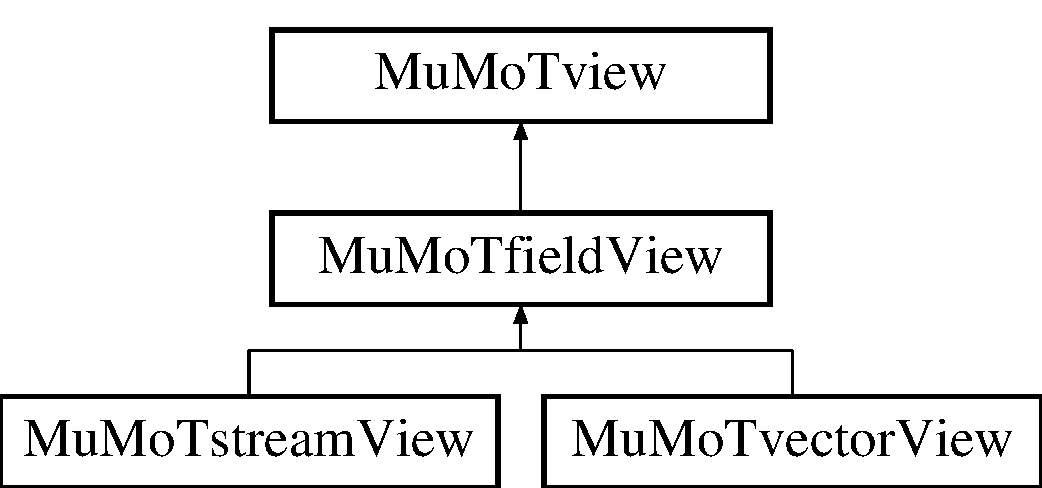
\includegraphics[height=3.000000cm]{class_mu_mo_t_1_1_mu_mo_tfield_view}
\end{center}
\end{figure}
\subsection*{Public Member Functions}
\begin{DoxyCompactItemize}
\item 
def \hyperlink{class_mu_mo_t_1_1_mu_mo_tfield_view_a78d68546a28ea07c46f5f4a44ddfa49a}{\+\_\+\+\_\+init\+\_\+\+\_\+} (self, model, controller, state\+Variable1, state\+Variable2, state\+Variable3=None, figure=None, params=None, kwargs)
\end{DoxyCompactItemize}
\subsection*{Private Member Functions}
\begin{DoxyCompactItemize}
\item 
def \hyperlink{class_mu_mo_t_1_1_mu_mo_tfield_view_a50d59419298116f738a98c864afb9d89}{\+\_\+plot\+\_\+field} (self)
\item 
def \hyperlink{class_mu_mo_t_1_1_mu_mo_tfield_view_aefbf0e354438e17ab6d48e2d368f8540}{\+\_\+get\+\_\+field} (self)
\begin{DoxyCompactList}\small\item\em helper for \+\_\+get\+\_\+field\+\_\+2d() and \+\_\+get\+\_\+field\+\_\+3d() \end{DoxyCompactList}\item 
def \hyperlink{class_mu_mo_t_1_1_mu_mo_tfield_view_a854f5f5badcda687eff8a999e6700cb7}{\+\_\+get\+\_\+field2d} (self, kind, mesh\+Points)
\begin{DoxyCompactList}\small\item\em get 2-\/dimensional field for plotting \end{DoxyCompactList}\item 
def \hyperlink{class_mu_mo_t_1_1_mu_mo_tfield_view_a7e92a660924e058d070dd1799c27f126}{\+\_\+get\+\_\+field3d} (self, kind, mesh\+Points)
\begin{DoxyCompactList}\small\item\em get 3-\/dimensional field for plotting \end{DoxyCompactList}\end{DoxyCompactItemize}
\subsection*{Private Attributes}
\begin{DoxyCompactItemize}
\item 
\hyperlink{class_mu_mo_t_1_1_mu_mo_tfield_view_a0f5fba57766067c941f5a96b22545ed4}{\+\_\+\+Xdot}
\item 
\hyperlink{class_mu_mo_t_1_1_mu_mo_tfield_view_a31f5ad9d4a349b00e06772177200c217}{\+\_\+\+Ydot}
\item 
\hyperlink{class_mu_mo_t_1_1_mu_mo_tfield_view_a4008c2e6651cb1bf1c9c1af3e962a25d}{\+\_\+\+Zdot}
\end{DoxyCompactItemize}
\subsection*{Static Private Attributes}
\begin{DoxyCompactItemize}
\item 
\hyperlink{class_mu_mo_t_1_1_mu_mo_tfield_view_aa14fa36730691becc6f3136899545416}{\+\_\+state\+Variable1} = None
\begin{DoxyCompactList}\small\item\em 1st state variable (x-\/dimension) \end{DoxyCompactList}\item 
\hyperlink{class_mu_mo_t_1_1_mu_mo_tfield_view_a9d3705d1d9182e10751ff693573d6d16}{\+\_\+state\+Variable2} = None
\begin{DoxyCompactList}\small\item\em 2nd state variable (y-\/dimension) \end{DoxyCompactList}\item 
\hyperlink{class_mu_mo_t_1_1_mu_mo_tfield_view_ad2f8dc44173a16468bd9d3ab335f9b27}{\+\_\+state\+Variable3} = None
\begin{DoxyCompactList}\small\item\em 3rd state variable (z-\/dimension) \end{DoxyCompactList}\item 
\hyperlink{class_mu_mo_t_1_1_mu_mo_tfield_view_abb529af75494ab2513e57b8434c7c975}{\+\_\+X} = None
\begin{DoxyCompactList}\small\item\em X ordinates array. \end{DoxyCompactList}\item 
\hyperlink{class_mu_mo_t_1_1_mu_mo_tfield_view_a17bd9f55d983ee8d5a6f22088d0397e8}{\+\_\+Y} = None
\begin{DoxyCompactList}\small\item\em Y ordinates array. \end{DoxyCompactList}\item 
\hyperlink{class_mu_mo_t_1_1_mu_mo_tfield_view_a7b96cbb62a4ad08851fa147958f0d6e4}{\+\_\+Z} = None
\begin{DoxyCompactList}\small\item\em Z ordinates array. \end{DoxyCompactList}\item 
\hyperlink{class_mu_mo_t_1_1_mu_mo_tfield_view_a3293b40663039bb46c8c977a9948436e}{\+\_\+speed} = None
\begin{DoxyCompactList}\small\item\em speed array \end{DoxyCompactList}\item 
dictionary \hyperlink{class_mu_mo_t_1_1_mu_mo_tfield_view_acbf4bc8fa26c3cf9e1d2741cc3dea058}{\+\_\+mask} = \{\}
\begin{DoxyCompactList}\small\item\em class-\/global dictionary of memoised masks with (mesh size, dimension) as key \end{DoxyCompactList}\end{DoxyCompactItemize}
\subsection*{Additional Inherited Members}


\subsection{Detailed Description}
field view on model (specialised by \hyperlink{class_mu_mo_t_1_1_mu_mo_tvector_view}{Mu\+Mo\+Tvector\+View} and \hyperlink{class_mu_mo_t_1_1_mu_mo_tstream_view}{Mu\+Mo\+Tstream\+View}) 

\subsection{Constructor \& Destructor Documentation}
\mbox{\Hypertarget{class_mu_mo_t_1_1_mu_mo_tfield_view_a78d68546a28ea07c46f5f4a44ddfa49a}\label{class_mu_mo_t_1_1_mu_mo_tfield_view_a78d68546a28ea07c46f5f4a44ddfa49a}} 
\index{Mu\+Mo\+T\+::\+Mu\+Mo\+Tfield\+View@{Mu\+Mo\+T\+::\+Mu\+Mo\+Tfield\+View}!\+\_\+\+\_\+init\+\_\+\+\_\+@{\+\_\+\+\_\+init\+\_\+\+\_\+}}
\index{\+\_\+\+\_\+init\+\_\+\+\_\+@{\+\_\+\+\_\+init\+\_\+\+\_\+}!Mu\+Mo\+T\+::\+Mu\+Mo\+Tfield\+View@{Mu\+Mo\+T\+::\+Mu\+Mo\+Tfield\+View}}
\subsubsection{\texorpdfstring{\+\_\+\+\_\+init\+\_\+\+\_\+()}{\_\_init\_\_()}}
{\footnotesize\ttfamily def \+\_\+\+\_\+init\+\_\+\+\_\+ (\begin{DoxyParamCaption}\item[{}]{self,  }\item[{}]{model,  }\item[{}]{controller,  }\item[{}]{state\+Variable1,  }\item[{}]{state\+Variable2,  }\item[{}]{state\+Variable3 = {\ttfamily None},  }\item[{}]{figure = {\ttfamily None},  }\item[{}]{params = {\ttfamily None},  }\item[{}]{kwargs }\end{DoxyParamCaption})}



\subsection{Member Function Documentation}
\mbox{\Hypertarget{class_mu_mo_t_1_1_mu_mo_tfield_view_aefbf0e354438e17ab6d48e2d368f8540}\label{class_mu_mo_t_1_1_mu_mo_tfield_view_aefbf0e354438e17ab6d48e2d368f8540}} 
\index{Mu\+Mo\+T\+::\+Mu\+Mo\+Tfield\+View@{Mu\+Mo\+T\+::\+Mu\+Mo\+Tfield\+View}!\+\_\+get\+\_\+field@{\+\_\+get\+\_\+field}}
\index{\+\_\+get\+\_\+field@{\+\_\+get\+\_\+field}!Mu\+Mo\+T\+::\+Mu\+Mo\+Tfield\+View@{Mu\+Mo\+T\+::\+Mu\+Mo\+Tfield\+View}}
\subsubsection{\texorpdfstring{\+\_\+get\+\_\+field()}{\_get\_field()}}
{\footnotesize\ttfamily def \+\_\+get\+\_\+field (\begin{DoxyParamCaption}\item[{}]{self }\end{DoxyParamCaption})\hspace{0.3cm}{\ttfamily [private]}}



helper for \+\_\+get\+\_\+field\+\_\+2d() and \+\_\+get\+\_\+field\+\_\+3d() 

\mbox{\Hypertarget{class_mu_mo_t_1_1_mu_mo_tfield_view_a854f5f5badcda687eff8a999e6700cb7}\label{class_mu_mo_t_1_1_mu_mo_tfield_view_a854f5f5badcda687eff8a999e6700cb7}} 
\index{Mu\+Mo\+T\+::\+Mu\+Mo\+Tfield\+View@{Mu\+Mo\+T\+::\+Mu\+Mo\+Tfield\+View}!\+\_\+get\+\_\+field2d@{\+\_\+get\+\_\+field2d}}
\index{\+\_\+get\+\_\+field2d@{\+\_\+get\+\_\+field2d}!Mu\+Mo\+T\+::\+Mu\+Mo\+Tfield\+View@{Mu\+Mo\+T\+::\+Mu\+Mo\+Tfield\+View}}
\subsubsection{\texorpdfstring{\+\_\+get\+\_\+field2d()}{\_get\_field2d()}}
{\footnotesize\ttfamily def \+\_\+get\+\_\+field2d (\begin{DoxyParamCaption}\item[{}]{self,  }\item[{}]{kind,  }\item[{}]{mesh\+Points }\end{DoxyParamCaption})\hspace{0.3cm}{\ttfamily [private]}}



get 2-\/dimensional field for plotting 

\mbox{\Hypertarget{class_mu_mo_t_1_1_mu_mo_tfield_view_a7e92a660924e058d070dd1799c27f126}\label{class_mu_mo_t_1_1_mu_mo_tfield_view_a7e92a660924e058d070dd1799c27f126}} 
\index{Mu\+Mo\+T\+::\+Mu\+Mo\+Tfield\+View@{Mu\+Mo\+T\+::\+Mu\+Mo\+Tfield\+View}!\+\_\+get\+\_\+field3d@{\+\_\+get\+\_\+field3d}}
\index{\+\_\+get\+\_\+field3d@{\+\_\+get\+\_\+field3d}!Mu\+Mo\+T\+::\+Mu\+Mo\+Tfield\+View@{Mu\+Mo\+T\+::\+Mu\+Mo\+Tfield\+View}}
\subsubsection{\texorpdfstring{\+\_\+get\+\_\+field3d()}{\_get\_field3d()}}
{\footnotesize\ttfamily def \+\_\+get\+\_\+field3d (\begin{DoxyParamCaption}\item[{}]{self,  }\item[{}]{kind,  }\item[{}]{mesh\+Points }\end{DoxyParamCaption})\hspace{0.3cm}{\ttfamily [private]}}



get 3-\/dimensional field for plotting 

\mbox{\Hypertarget{class_mu_mo_t_1_1_mu_mo_tfield_view_a50d59419298116f738a98c864afb9d89}\label{class_mu_mo_t_1_1_mu_mo_tfield_view_a50d59419298116f738a98c864afb9d89}} 
\index{Mu\+Mo\+T\+::\+Mu\+Mo\+Tfield\+View@{Mu\+Mo\+T\+::\+Mu\+Mo\+Tfield\+View}!\+\_\+plot\+\_\+field@{\+\_\+plot\+\_\+field}}
\index{\+\_\+plot\+\_\+field@{\+\_\+plot\+\_\+field}!Mu\+Mo\+T\+::\+Mu\+Mo\+Tfield\+View@{Mu\+Mo\+T\+::\+Mu\+Mo\+Tfield\+View}}
\subsubsection{\texorpdfstring{\+\_\+plot\+\_\+field()}{\_plot\_field()}}
{\footnotesize\ttfamily def \+\_\+plot\+\_\+field (\begin{DoxyParamCaption}\item[{}]{self }\end{DoxyParamCaption})\hspace{0.3cm}{\ttfamily [private]}}



\subsection{Field Documentation}
\mbox{\Hypertarget{class_mu_mo_t_1_1_mu_mo_tfield_view_acbf4bc8fa26c3cf9e1d2741cc3dea058}\label{class_mu_mo_t_1_1_mu_mo_tfield_view_acbf4bc8fa26c3cf9e1d2741cc3dea058}} 
\index{Mu\+Mo\+T\+::\+Mu\+Mo\+Tfield\+View@{Mu\+Mo\+T\+::\+Mu\+Mo\+Tfield\+View}!\+\_\+mask@{\+\_\+mask}}
\index{\+\_\+mask@{\+\_\+mask}!Mu\+Mo\+T\+::\+Mu\+Mo\+Tfield\+View@{Mu\+Mo\+T\+::\+Mu\+Mo\+Tfield\+View}}
\subsubsection{\texorpdfstring{\+\_\+mask}{\_mask}}
{\footnotesize\ttfamily dictionary \+\_\+mask = \{\}\hspace{0.3cm}{\ttfamily [static]}, {\ttfamily [private]}}



class-\/global dictionary of memoised masks with (mesh size, dimension) as key 

\mbox{\Hypertarget{class_mu_mo_t_1_1_mu_mo_tfield_view_a3293b40663039bb46c8c977a9948436e}\label{class_mu_mo_t_1_1_mu_mo_tfield_view_a3293b40663039bb46c8c977a9948436e}} 
\index{Mu\+Mo\+T\+::\+Mu\+Mo\+Tfield\+View@{Mu\+Mo\+T\+::\+Mu\+Mo\+Tfield\+View}!\+\_\+speed@{\+\_\+speed}}
\index{\+\_\+speed@{\+\_\+speed}!Mu\+Mo\+T\+::\+Mu\+Mo\+Tfield\+View@{Mu\+Mo\+T\+::\+Mu\+Mo\+Tfield\+View}}
\subsubsection{\texorpdfstring{\+\_\+speed}{\_speed}}
{\footnotesize\ttfamily \+\_\+speed = None\hspace{0.3cm}{\ttfamily [static]}, {\ttfamily [private]}}



speed array 

\mbox{\Hypertarget{class_mu_mo_t_1_1_mu_mo_tfield_view_aa14fa36730691becc6f3136899545416}\label{class_mu_mo_t_1_1_mu_mo_tfield_view_aa14fa36730691becc6f3136899545416}} 
\index{Mu\+Mo\+T\+::\+Mu\+Mo\+Tfield\+View@{Mu\+Mo\+T\+::\+Mu\+Mo\+Tfield\+View}!\+\_\+state\+Variable1@{\+\_\+state\+Variable1}}
\index{\+\_\+state\+Variable1@{\+\_\+state\+Variable1}!Mu\+Mo\+T\+::\+Mu\+Mo\+Tfield\+View@{Mu\+Mo\+T\+::\+Mu\+Mo\+Tfield\+View}}
\subsubsection{\texorpdfstring{\+\_\+state\+Variable1}{\_stateVariable1}}
{\footnotesize\ttfamily \+\_\+state\+Variable1 = None\hspace{0.3cm}{\ttfamily [static]}, {\ttfamily [private]}}



1st state variable (x-\/dimension) 

\mbox{\Hypertarget{class_mu_mo_t_1_1_mu_mo_tfield_view_a9d3705d1d9182e10751ff693573d6d16}\label{class_mu_mo_t_1_1_mu_mo_tfield_view_a9d3705d1d9182e10751ff693573d6d16}} 
\index{Mu\+Mo\+T\+::\+Mu\+Mo\+Tfield\+View@{Mu\+Mo\+T\+::\+Mu\+Mo\+Tfield\+View}!\+\_\+state\+Variable2@{\+\_\+state\+Variable2}}
\index{\+\_\+state\+Variable2@{\+\_\+state\+Variable2}!Mu\+Mo\+T\+::\+Mu\+Mo\+Tfield\+View@{Mu\+Mo\+T\+::\+Mu\+Mo\+Tfield\+View}}
\subsubsection{\texorpdfstring{\+\_\+state\+Variable2}{\_stateVariable2}}
{\footnotesize\ttfamily \+\_\+state\+Variable2 = None\hspace{0.3cm}{\ttfamily [static]}, {\ttfamily [private]}}



2nd state variable (y-\/dimension) 

\mbox{\Hypertarget{class_mu_mo_t_1_1_mu_mo_tfield_view_ad2f8dc44173a16468bd9d3ab335f9b27}\label{class_mu_mo_t_1_1_mu_mo_tfield_view_ad2f8dc44173a16468bd9d3ab335f9b27}} 
\index{Mu\+Mo\+T\+::\+Mu\+Mo\+Tfield\+View@{Mu\+Mo\+T\+::\+Mu\+Mo\+Tfield\+View}!\+\_\+state\+Variable3@{\+\_\+state\+Variable3}}
\index{\+\_\+state\+Variable3@{\+\_\+state\+Variable3}!Mu\+Mo\+T\+::\+Mu\+Mo\+Tfield\+View@{Mu\+Mo\+T\+::\+Mu\+Mo\+Tfield\+View}}
\subsubsection{\texorpdfstring{\+\_\+state\+Variable3}{\_stateVariable3}}
{\footnotesize\ttfamily \+\_\+state\+Variable3 = None\hspace{0.3cm}{\ttfamily [static]}, {\ttfamily [private]}}



3rd state variable (z-\/dimension) 

\mbox{\Hypertarget{class_mu_mo_t_1_1_mu_mo_tfield_view_abb529af75494ab2513e57b8434c7c975}\label{class_mu_mo_t_1_1_mu_mo_tfield_view_abb529af75494ab2513e57b8434c7c975}} 
\index{Mu\+Mo\+T\+::\+Mu\+Mo\+Tfield\+View@{Mu\+Mo\+T\+::\+Mu\+Mo\+Tfield\+View}!\+\_\+X@{\+\_\+X}}
\index{\+\_\+X@{\+\_\+X}!Mu\+Mo\+T\+::\+Mu\+Mo\+Tfield\+View@{Mu\+Mo\+T\+::\+Mu\+Mo\+Tfield\+View}}
\subsubsection{\texorpdfstring{\+\_\+X}{\_X}}
{\footnotesize\ttfamily \+\_\+X = None\hspace{0.3cm}{\ttfamily [static]}, {\ttfamily [private]}}



X ordinates array. 

X derivatives array. \mbox{\Hypertarget{class_mu_mo_t_1_1_mu_mo_tfield_view_a0f5fba57766067c941f5a96b22545ed4}\label{class_mu_mo_t_1_1_mu_mo_tfield_view_a0f5fba57766067c941f5a96b22545ed4}} 
\index{Mu\+Mo\+T\+::\+Mu\+Mo\+Tfield\+View@{Mu\+Mo\+T\+::\+Mu\+Mo\+Tfield\+View}!\+\_\+\+Xdot@{\+\_\+\+Xdot}}
\index{\+\_\+\+Xdot@{\+\_\+\+Xdot}!Mu\+Mo\+T\+::\+Mu\+Mo\+Tfield\+View@{Mu\+Mo\+T\+::\+Mu\+Mo\+Tfield\+View}}
\subsubsection{\texorpdfstring{\+\_\+\+Xdot}{\_Xdot}}
{\footnotesize\ttfamily \+\_\+\+Xdot\hspace{0.3cm}{\ttfamily [private]}}

\begin{DoxyRefDesc}{Todo}
\item[\hyperlink{todo__todo000031}{Todo}]system size defined to be one \end{DoxyRefDesc}
\begin{DoxyRefDesc}{Todo}
\item[\hyperlink{todo__todo000032}{Todo}]\+: allow user to set mesh points with keyword \end{DoxyRefDesc}


\begin{DoxyRefDesc}{Todo}
\item[\hyperlink{todo__todo000033}{Todo}]system size defined to be one \end{DoxyRefDesc}
\mbox{\Hypertarget{class_mu_mo_t_1_1_mu_mo_tfield_view_a17bd9f55d983ee8d5a6f22088d0397e8}\label{class_mu_mo_t_1_1_mu_mo_tfield_view_a17bd9f55d983ee8d5a6f22088d0397e8}} 
\index{Mu\+Mo\+T\+::\+Mu\+Mo\+Tfield\+View@{Mu\+Mo\+T\+::\+Mu\+Mo\+Tfield\+View}!\+\_\+Y@{\+\_\+Y}}
\index{\+\_\+Y@{\+\_\+Y}!Mu\+Mo\+T\+::\+Mu\+Mo\+Tfield\+View@{Mu\+Mo\+T\+::\+Mu\+Mo\+Tfield\+View}}
\subsubsection{\texorpdfstring{\+\_\+Y}{\_Y}}
{\footnotesize\ttfamily \+\_\+Y = None\hspace{0.3cm}{\ttfamily [static]}, {\ttfamily [private]}}



Y ordinates array. 

Y derivatives array. \mbox{\Hypertarget{class_mu_mo_t_1_1_mu_mo_tfield_view_a31f5ad9d4a349b00e06772177200c217}\label{class_mu_mo_t_1_1_mu_mo_tfield_view_a31f5ad9d4a349b00e06772177200c217}} 
\index{Mu\+Mo\+T\+::\+Mu\+Mo\+Tfield\+View@{Mu\+Mo\+T\+::\+Mu\+Mo\+Tfield\+View}!\+\_\+\+Ydot@{\+\_\+\+Ydot}}
\index{\+\_\+\+Ydot@{\+\_\+\+Ydot}!Mu\+Mo\+T\+::\+Mu\+Mo\+Tfield\+View@{Mu\+Mo\+T\+::\+Mu\+Mo\+Tfield\+View}}
\subsubsection{\texorpdfstring{\+\_\+\+Ydot}{\_Ydot}}
{\footnotesize\ttfamily \+\_\+\+Ydot\hspace{0.3cm}{\ttfamily [private]}}

\mbox{\Hypertarget{class_mu_mo_t_1_1_mu_mo_tfield_view_a7b96cbb62a4ad08851fa147958f0d6e4}\label{class_mu_mo_t_1_1_mu_mo_tfield_view_a7b96cbb62a4ad08851fa147958f0d6e4}} 
\index{Mu\+Mo\+T\+::\+Mu\+Mo\+Tfield\+View@{Mu\+Mo\+T\+::\+Mu\+Mo\+Tfield\+View}!\+\_\+Z@{\+\_\+Z}}
\index{\+\_\+Z@{\+\_\+Z}!Mu\+Mo\+T\+::\+Mu\+Mo\+Tfield\+View@{Mu\+Mo\+T\+::\+Mu\+Mo\+Tfield\+View}}
\subsubsection{\texorpdfstring{\+\_\+Z}{\_Z}}
{\footnotesize\ttfamily \+\_\+Z = None\hspace{0.3cm}{\ttfamily [static]}, {\ttfamily [private]}}



Z ordinates array. 

Z derivatives array. \mbox{\Hypertarget{class_mu_mo_t_1_1_mu_mo_tfield_view_a4008c2e6651cb1bf1c9c1af3e962a25d}\label{class_mu_mo_t_1_1_mu_mo_tfield_view_a4008c2e6651cb1bf1c9c1af3e962a25d}} 
\index{Mu\+Mo\+T\+::\+Mu\+Mo\+Tfield\+View@{Mu\+Mo\+T\+::\+Mu\+Mo\+Tfield\+View}!\+\_\+\+Zdot@{\+\_\+\+Zdot}}
\index{\+\_\+\+Zdot@{\+\_\+\+Zdot}!Mu\+Mo\+T\+::\+Mu\+Mo\+Tfield\+View@{Mu\+Mo\+T\+::\+Mu\+Mo\+Tfield\+View}}
\subsubsection{\texorpdfstring{\+\_\+\+Zdot}{\_Zdot}}
{\footnotesize\ttfamily \+\_\+\+Zdot\hspace{0.3cm}{\ttfamily [private]}}



The documentation for this class was generated from the following file\+:\begin{DoxyCompactItemize}
\item 
\hyperlink{_mu_mo_t_8py}{Mu\+Mo\+T.\+py}\end{DoxyCompactItemize}

\hypertarget{class_mu_mo_t_1_1_mu_mo_tmodel}{}\section{Mu\+Mo\+Tmodel Class Reference}
\label{class_mu_mo_t_1_1_mu_mo_tmodel}\index{Mu\+Mo\+Tmodel@{Mu\+Mo\+Tmodel}}


class describing a model  


\subsection*{Public Member Functions}
\begin{DoxyCompactItemize}
\item 
def \hyperlink{class_mu_mo_t_1_1_mu_mo_tmodel_a2eec4a3b8deda7c717c06ed89c24d570}{substitute} (self, subs\+String)
\begin{DoxyCompactList}\small\item\em create new model with variable substitutions listed as comma separated string of assignments \end{DoxyCompactList}\item 
def \hyperlink{class_mu_mo_t_1_1_mu_mo_tmodel_affc6fae7ea26f85cde5366af8af85200}{visualise} (self)
\begin{DoxyCompactList}\small\item\em build a graphical representation of the model if result cannot be plotted check for installation of libltdl -\/ eg on Mac see if X\+Quartz requires update or do\+:~\newline
 {\ttfamily brew install libtool -\/-\/universal} ~\newline
 {\ttfamily brew link libtool} \end{DoxyCompactList}\item 
def \hyperlink{class_mu_mo_t_1_1_mu_mo_tmodel_a2feaf6de25201c1e6503cd2ed131a1f2}{show\+Reactants} (self)
\begin{DoxyCompactList}\small\item\em show a sorted La\+TeX representation of the model\textquotesingle{}s reactants \end{DoxyCompactList}\item 
def \hyperlink{class_mu_mo_t_1_1_mu_mo_tmodel_a9c88600ec8eda7be7b7faeacd99f1682}{show\+Rates} (self)
\begin{DoxyCompactList}\small\item\em show a sorted La\+TeX representation of the model\textquotesingle{}s rate parameters \end{DoxyCompactList}\item 
def \hyperlink{class_mu_mo_t_1_1_mu_mo_tmodel_aa3a519a3aac92f7c132c63fb12d3de13}{show\+O\+D\+Es} (self)
\begin{DoxyCompactList}\small\item\em show a La\+TeX representation of the model system of O\+D\+Es \end{DoxyCompactList}\item 
def \hyperlink{class_mu_mo_t_1_1_mu_mo_tmodel_ab4f4398c3f210fe4ea6e720401357691}{show} (self)
\item 
def \hyperlink{class_mu_mo_t_1_1_mu_mo_tmodel_ae2925a9a37b83608167da0794fe1a2a8}{stream} (self, state\+Variable1, state\+Variable2, state\+Variable3=None, kwargs)
\begin{DoxyCompactList}\small\item\em construct interactive stream plot \end{DoxyCompactList}\item 
def \hyperlink{class_mu_mo_t_1_1_mu_mo_tmodel_aa7a2f83702a081cec49e9f18d8392830}{vector} (self, state\+Variable1, state\+Variable2, state\+Variable3=None, kwargs)
\begin{DoxyCompactList}\small\item\em construct interactive vector plot \end{DoxyCompactList}\item 
def \hyperlink{class_mu_mo_t_1_1_mu_mo_tmodel_a41de1154182c3807821a722c4b91e824}{bifurcation} (self, bifurcation\+Parameter, state\+Variable1, state\+Variable2=None, kwargs)
\begin{DoxyCompactList}\small\item\em construct interactive Py\+D\+S\+Tool plot \end{DoxyCompactList}\item 
def \hyperlink{class_mu_mo_t_1_1_mu_mo_tmodel_a55f7cab206306b09d38863395f186dbc}{multiagent} (self, net\+Type=\char`\"{}full\char`\"{}, initial\+State=\char`\"{}Auto\char`\"{}, max\+Time=\char`\"{}Auto\char`\"{}, random\+Seed=\char`\"{}Auto\char`\"{}, kwargs)
\item 
def \hyperlink{class_mu_mo_t_1_1_mu_mo_tmodel_ac3c78f7f98887f29a4f0d50dd023c465}{S\+SA} (self, initial\+State=\char`\"{}Auto\char`\"{}, max\+Time=\char`\"{}Auto\char`\"{}, random\+Seed=\char`\"{}Auto\char`\"{}, kwargs)
\item 
def \hyperlink{class_mu_mo_t_1_1_mu_mo_tmodel_ae64f0875afe3067b97ba370b354b9213}{\+\_\+\+\_\+init\+\_\+\+\_\+} (self)
\item 
def \hyperlink{class_mu_mo_t_1_1_mu_mo_tmodel_a41a65d7030dd1006b177d0bc24e1a12b}{\+\_\+\+\_\+del\+\_\+\+\_\+} (self)
\end{DoxyCompactItemize}
\subsection*{Private Member Functions}
\begin{DoxyCompactItemize}
\item 
def \hyperlink{class_mu_mo_t_1_1_mu_mo_tmodel_ac8f6319b8c81e7c48d1f892603bcd307}{\+\_\+get\+\_\+solutions} (self)
\item 
def \hyperlink{class_mu_mo_t_1_1_mu_mo_tmodel_a858789fcc57b8480f22e2a6f4446d94e}{\+\_\+controller} (self, cont\+Refresh, kwargs)
\begin{DoxyCompactList}\small\item\em general controller constructor with all rates as free parameters \end{DoxyCompactList}\item 
def \hyperlink{class_mu_mo_t_1_1_mu_mo_tmodel_abef2b7019d8de30c16d7ade84ad45e09}{\+\_\+check\+\_\+state\+\_\+variables} (self, state\+Variable1, state\+Variable2, state\+Variable3=None)
\item 
def \hyperlink{class_mu_mo_t_1_1_mu_mo_tmodel_aa69fe5568e12577be5a63232d689e45e}{\+\_\+get\+Funcs} (self)
\begin{DoxyCompactList}\small\item\em lambdify sympy equations for numerical integration, plotting, etc. \end{DoxyCompactList}\item 
def \hyperlink{class_mu_mo_t_1_1_mu_mo_tmodel_a0965e5e61aa8f0d4e399e3b534d31a4c}{\+\_\+get\+Arg\+Tuple2d} (self, arg\+Names, arg\+Values, arg\+Dict, state\+Variable1, state\+Variable2, X, Y)
\begin{DoxyCompactList}\small\item\em get tuple to evalute functions returned by \+\_\+get\+Funcs with, for 2d field-\/based plots \end{DoxyCompactList}\item 
def \hyperlink{class_mu_mo_t_1_1_mu_mo_tmodel_a4a81885dd0451b6af31285c234b61d2a}{\+\_\+get\+Arg\+Tuple3d} (self, arg\+Names, arg\+Values, arg\+Dict, state\+Variable1, state\+Variable2, state\+Variable3, X, Y, Z)
\begin{DoxyCompactList}\small\item\em get tuple to evalute functions returned by \+\_\+get\+Funcs with, for 2d field-\/based plots \end{DoxyCompactList}\item 
def \hyperlink{class_mu_mo_t_1_1_mu_mo_tmodel_af547c59d7ec82de308ee85b118fc7295}{\+\_\+get\+Arg\+Tuple} (self, arg\+Names, arg\+Values, arg\+Dict, reactants, reactant\+Values)
\begin{DoxyCompactList}\small\item\em get tuple to evalute functions returned by \+\_\+get\+Funcs with \end{DoxyCompactList}\item 
def \hyperlink{class_mu_mo_t_1_1_mu_mo_tmodel_ad1478cdd69a86f50f84e0528f829573c}{\+\_\+local\+La\+Te\+Ximage\+File} (self, source)
\begin{DoxyCompactList}\small\item\em render La\+TeX source to local image file \end{DoxyCompactList}\end{DoxyCompactItemize}
\subsection*{Private Attributes}
\begin{DoxyCompactItemize}
\item 
\hyperlink{class_mu_mo_t_1_1_mu_mo_tmodel_a9e9a430da6d323cc4411c070e0c7eee5}{\+\_\+py\+D\+Smodel}
\end{DoxyCompactItemize}
\subsection*{Static Private Attributes}
\begin{DoxyCompactItemize}
\item 
\hyperlink{class_mu_mo_t_1_1_mu_mo_tmodel_a3bffcba47fea374758cdf6e1abc66b6a}{\+\_\+rules} = None
\begin{DoxyCompactList}\small\item\em list of rules \end{DoxyCompactList}\item 
\hyperlink{class_mu_mo_t_1_1_mu_mo_tmodel_ab78b4926218dd610cd20b0fd9816f96b}{\+\_\+reactants} = None
\begin{DoxyCompactList}\small\item\em set of reactants \end{DoxyCompactList}\item 
\hyperlink{class_mu_mo_t_1_1_mu_mo_tmodel_afaae7e86425ed04f1e39b4bb8039b1b4}{\+\_\+system\+Size} = None
\begin{DoxyCompactList}\small\item\em parameter that determines system size, set by using \hyperlink{class_mu_mo_t_1_1_mu_mo_tmodel_a2eec4a3b8deda7c717c06ed89c24d570}{substitute()} \end{DoxyCompactList}\item 
\hyperlink{class_mu_mo_t_1_1_mu_mo_tmodel_accfd4bbcd94ec3ce4a064fec53921700}{\+\_\+reactants\+La\+TeX} = None
\begin{DoxyCompactList}\small\item\em list of La\+TeX strings describing reactants ( \end{DoxyCompactList}\item 
\hyperlink{class_mu_mo_t_1_1_mu_mo_tmodel_a45fe1a3c95be7c7db64a0199619569a9}{\+\_\+rates} = None
\begin{DoxyCompactList}\small\item\em set of rates \end{DoxyCompactList}\item 
\hyperlink{class_mu_mo_t_1_1_mu_mo_tmodel_a795ce014c05817c0ac931270e961020f}{\+\_\+rates\+La\+TeX} = None
\begin{DoxyCompactList}\small\item\em dictionary of La\+TeX strings describing rates \end{DoxyCompactList}\item 
\hyperlink{class_mu_mo_t_1_1_mu_mo_tmodel_ab9682b098aac7aac3179a3773749fd71}{\+\_\+equations} = None
\begin{DoxyCompactList}\small\item\em dictionary of O\+DE righthand sides with reactant as key \end{DoxyCompactList}\item 
\hyperlink{class_mu_mo_t_1_1_mu_mo_tmodel_a31c9407d55747598fa4c9efdd6f9293d}{\+\_\+solutions} = None
\begin{DoxyCompactList}\small\item\em set of solutions to equations \end{DoxyCompactList}\item 
\hyperlink{class_mu_mo_t_1_1_mu_mo_tmodel_a8ef9f9e4473f46043da1484716b18268}{\+\_\+funcs} = None
\begin{DoxyCompactList}\small\item\em dictionary of lambdified functions for integration, plotting, etc. \end{DoxyCompactList}\item 
\hyperlink{class_mu_mo_t_1_1_mu_mo_tmodel_a04c0353d4e8a6c3f2e0a1fb36ed9a832}{\+\_\+args} = None
\begin{DoxyCompactList}\small\item\em tuple of argument symbols for lambdified functions \end{DoxyCompactList}\item 
\hyperlink{class_mu_mo_t_1_1_mu_mo_tmodel_aaabcff4440dc0ded9f9f880c9f86c6c1}{\+\_\+dot} = None
\begin{DoxyCompactList}\small\item\em graphviz visualisation of model \end{DoxyCompactList}\item 
string \hyperlink{class_mu_mo_t_1_1_mu_mo_tmodel_a385c519c2aed996e4bad454f870fed0c}{\+\_\+render\+Image\+Format} = \textquotesingle{}png\textquotesingle{}
\begin{DoxyCompactList}\small\item\em image format used for rendering edge labels for model visualisation \end{DoxyCompactList}\item 
string \hyperlink{class_mu_mo_t_1_1_mu_mo_tmodel_a4ac4f3325e967c92d03e2c4e023a0d5d}{\+\_\+tmpdirpath} = \textquotesingle{}\+\_\+\+\_\+mumot\+\_\+files\+\_\+\+\_\+\textquotesingle{}
\begin{DoxyCompactList}\small\item\em local path for creation of temporary storage \end{DoxyCompactList}\item 
\hyperlink{class_mu_mo_t_1_1_mu_mo_tmodel_ad2feb50403a36ab7c591c04e0cf33cc4}{\+\_\+tmpdir} = None
\begin{DoxyCompactList}\small\item\em temporary storage for image files, etc. \end{DoxyCompactList}\item 
\hyperlink{class_mu_mo_t_1_1_mu_mo_tmodel_a3f2d20ce626e9e6cdc4a4662727121e6}{\+\_\+tmpfiles} = None
\begin{DoxyCompactList}\small\item\em list of temporary files created \end{DoxyCompactList}\end{DoxyCompactItemize}


\subsection{Detailed Description}
class describing a model 

\subsection{Constructor \& Destructor Documentation}
\mbox{\Hypertarget{class_mu_mo_t_1_1_mu_mo_tmodel_ae64f0875afe3067b97ba370b354b9213}\label{class_mu_mo_t_1_1_mu_mo_tmodel_ae64f0875afe3067b97ba370b354b9213}} 
\index{Mu\+Mo\+T\+::\+Mu\+Mo\+Tmodel@{Mu\+Mo\+T\+::\+Mu\+Mo\+Tmodel}!\+\_\+\+\_\+init\+\_\+\+\_\+@{\+\_\+\+\_\+init\+\_\+\+\_\+}}
\index{\+\_\+\+\_\+init\+\_\+\+\_\+@{\+\_\+\+\_\+init\+\_\+\+\_\+}!Mu\+Mo\+T\+::\+Mu\+Mo\+Tmodel@{Mu\+Mo\+T\+::\+Mu\+Mo\+Tmodel}}
\subsubsection{\texorpdfstring{\+\_\+\+\_\+init\+\_\+\+\_\+()}{\_\_init\_\_()}}
{\footnotesize\ttfamily def \+\_\+\+\_\+init\+\_\+\+\_\+ (\begin{DoxyParamCaption}\item[{}]{self }\end{DoxyParamCaption})}

\mbox{\Hypertarget{class_mu_mo_t_1_1_mu_mo_tmodel_a41a65d7030dd1006b177d0bc24e1a12b}\label{class_mu_mo_t_1_1_mu_mo_tmodel_a41a65d7030dd1006b177d0bc24e1a12b}} 
\index{Mu\+Mo\+T\+::\+Mu\+Mo\+Tmodel@{Mu\+Mo\+T\+::\+Mu\+Mo\+Tmodel}!\+\_\+\+\_\+del\+\_\+\+\_\+@{\+\_\+\+\_\+del\+\_\+\+\_\+}}
\index{\+\_\+\+\_\+del\+\_\+\+\_\+@{\+\_\+\+\_\+del\+\_\+\+\_\+}!Mu\+Mo\+T\+::\+Mu\+Mo\+Tmodel@{Mu\+Mo\+T\+::\+Mu\+Mo\+Tmodel}}
\subsubsection{\texorpdfstring{\+\_\+\+\_\+del\+\_\+\+\_\+()}{\_\_del\_\_()}}
{\footnotesize\ttfamily def \+\_\+\+\_\+del\+\_\+\+\_\+ (\begin{DoxyParamCaption}\item[{}]{self }\end{DoxyParamCaption})}



\subsection{Member Function Documentation}
\mbox{\Hypertarget{class_mu_mo_t_1_1_mu_mo_tmodel_abef2b7019d8de30c16d7ade84ad45e09}\label{class_mu_mo_t_1_1_mu_mo_tmodel_abef2b7019d8de30c16d7ade84ad45e09}} 
\index{Mu\+Mo\+T\+::\+Mu\+Mo\+Tmodel@{Mu\+Mo\+T\+::\+Mu\+Mo\+Tmodel}!\+\_\+check\+\_\+state\+\_\+variables@{\+\_\+check\+\_\+state\+\_\+variables}}
\index{\+\_\+check\+\_\+state\+\_\+variables@{\+\_\+check\+\_\+state\+\_\+variables}!Mu\+Mo\+T\+::\+Mu\+Mo\+Tmodel@{Mu\+Mo\+T\+::\+Mu\+Mo\+Tmodel}}
\subsubsection{\texorpdfstring{\+\_\+check\+\_\+state\+\_\+variables()}{\_check\_state\_variables()}}
{\footnotesize\ttfamily def \+\_\+check\+\_\+state\+\_\+variables (\begin{DoxyParamCaption}\item[{}]{self,  }\item[{}]{state\+Variable1,  }\item[{}]{state\+Variable2,  }\item[{}]{state\+Variable3 = {\ttfamily None} }\end{DoxyParamCaption})\hspace{0.3cm}{\ttfamily [private]}}

\mbox{\Hypertarget{class_mu_mo_t_1_1_mu_mo_tmodel_a858789fcc57b8480f22e2a6f4446d94e}\label{class_mu_mo_t_1_1_mu_mo_tmodel_a858789fcc57b8480f22e2a6f4446d94e}} 
\index{Mu\+Mo\+T\+::\+Mu\+Mo\+Tmodel@{Mu\+Mo\+T\+::\+Mu\+Mo\+Tmodel}!\+\_\+controller@{\+\_\+controller}}
\index{\+\_\+controller@{\+\_\+controller}!Mu\+Mo\+T\+::\+Mu\+Mo\+Tmodel@{Mu\+Mo\+T\+::\+Mu\+Mo\+Tmodel}}
\subsubsection{\texorpdfstring{\+\_\+controller()}{\_controller()}}
{\footnotesize\ttfamily def \+\_\+controller (\begin{DoxyParamCaption}\item[{}]{self,  }\item[{}]{cont\+Refresh,  }\item[{}]{kwargs }\end{DoxyParamCaption})\hspace{0.3cm}{\ttfamily [private]}}



general controller constructor with all rates as free parameters 

\mbox{\Hypertarget{class_mu_mo_t_1_1_mu_mo_tmodel_ac8f6319b8c81e7c48d1f892603bcd307}\label{class_mu_mo_t_1_1_mu_mo_tmodel_ac8f6319b8c81e7c48d1f892603bcd307}} 
\index{Mu\+Mo\+T\+::\+Mu\+Mo\+Tmodel@{Mu\+Mo\+T\+::\+Mu\+Mo\+Tmodel}!\+\_\+get\+\_\+solutions@{\+\_\+get\+\_\+solutions}}
\index{\+\_\+get\+\_\+solutions@{\+\_\+get\+\_\+solutions}!Mu\+Mo\+T\+::\+Mu\+Mo\+Tmodel@{Mu\+Mo\+T\+::\+Mu\+Mo\+Tmodel}}
\subsubsection{\texorpdfstring{\+\_\+get\+\_\+solutions()}{\_get\_solutions()}}
{\footnotesize\ttfamily def \+\_\+get\+\_\+solutions (\begin{DoxyParamCaption}\item[{}]{self }\end{DoxyParamCaption})\hspace{0.3cm}{\ttfamily [private]}}

\mbox{\Hypertarget{class_mu_mo_t_1_1_mu_mo_tmodel_af547c59d7ec82de308ee85b118fc7295}\label{class_mu_mo_t_1_1_mu_mo_tmodel_af547c59d7ec82de308ee85b118fc7295}} 
\index{Mu\+Mo\+T\+::\+Mu\+Mo\+Tmodel@{Mu\+Mo\+T\+::\+Mu\+Mo\+Tmodel}!\+\_\+get\+Arg\+Tuple@{\+\_\+get\+Arg\+Tuple}}
\index{\+\_\+get\+Arg\+Tuple@{\+\_\+get\+Arg\+Tuple}!Mu\+Mo\+T\+::\+Mu\+Mo\+Tmodel@{Mu\+Mo\+T\+::\+Mu\+Mo\+Tmodel}}
\subsubsection{\texorpdfstring{\+\_\+get\+Arg\+Tuple()}{\_getArgTuple()}}
{\footnotesize\ttfamily def \+\_\+get\+Arg\+Tuple (\begin{DoxyParamCaption}\item[{}]{self,  }\item[{}]{arg\+Names,  }\item[{}]{arg\+Values,  }\item[{}]{arg\+Dict,  }\item[{}]{reactants,  }\item[{}]{reactant\+Values }\end{DoxyParamCaption})\hspace{0.3cm}{\ttfamily [private]}}



get tuple to evalute functions returned by \+\_\+get\+Funcs with 

\mbox{\Hypertarget{class_mu_mo_t_1_1_mu_mo_tmodel_a0965e5e61aa8f0d4e399e3b534d31a4c}\label{class_mu_mo_t_1_1_mu_mo_tmodel_a0965e5e61aa8f0d4e399e3b534d31a4c}} 
\index{Mu\+Mo\+T\+::\+Mu\+Mo\+Tmodel@{Mu\+Mo\+T\+::\+Mu\+Mo\+Tmodel}!\+\_\+get\+Arg\+Tuple2d@{\+\_\+get\+Arg\+Tuple2d}}
\index{\+\_\+get\+Arg\+Tuple2d@{\+\_\+get\+Arg\+Tuple2d}!Mu\+Mo\+T\+::\+Mu\+Mo\+Tmodel@{Mu\+Mo\+T\+::\+Mu\+Mo\+Tmodel}}
\subsubsection{\texorpdfstring{\+\_\+get\+Arg\+Tuple2d()}{\_getArgTuple2d()}}
{\footnotesize\ttfamily def \+\_\+get\+Arg\+Tuple2d (\begin{DoxyParamCaption}\item[{}]{self,  }\item[{}]{arg\+Names,  }\item[{}]{arg\+Values,  }\item[{}]{arg\+Dict,  }\item[{}]{state\+Variable1,  }\item[{}]{state\+Variable2,  }\item[{}]{X,  }\item[{}]{Y }\end{DoxyParamCaption})\hspace{0.3cm}{\ttfamily [private]}}



get tuple to evalute functions returned by \+\_\+get\+Funcs with, for 2d field-\/based plots 

\mbox{\Hypertarget{class_mu_mo_t_1_1_mu_mo_tmodel_a4a81885dd0451b6af31285c234b61d2a}\label{class_mu_mo_t_1_1_mu_mo_tmodel_a4a81885dd0451b6af31285c234b61d2a}} 
\index{Mu\+Mo\+T\+::\+Mu\+Mo\+Tmodel@{Mu\+Mo\+T\+::\+Mu\+Mo\+Tmodel}!\+\_\+get\+Arg\+Tuple3d@{\+\_\+get\+Arg\+Tuple3d}}
\index{\+\_\+get\+Arg\+Tuple3d@{\+\_\+get\+Arg\+Tuple3d}!Mu\+Mo\+T\+::\+Mu\+Mo\+Tmodel@{Mu\+Mo\+T\+::\+Mu\+Mo\+Tmodel}}
\subsubsection{\texorpdfstring{\+\_\+get\+Arg\+Tuple3d()}{\_getArgTuple3d()}}
{\footnotesize\ttfamily def \+\_\+get\+Arg\+Tuple3d (\begin{DoxyParamCaption}\item[{}]{self,  }\item[{}]{arg\+Names,  }\item[{}]{arg\+Values,  }\item[{}]{arg\+Dict,  }\item[{}]{state\+Variable1,  }\item[{}]{state\+Variable2,  }\item[{}]{state\+Variable3,  }\item[{}]{X,  }\item[{}]{Y,  }\item[{}]{Z }\end{DoxyParamCaption})\hspace{0.3cm}{\ttfamily [private]}}



get tuple to evalute functions returned by \+\_\+get\+Funcs with, for 2d field-\/based plots 

\mbox{\Hypertarget{class_mu_mo_t_1_1_mu_mo_tmodel_aa69fe5568e12577be5a63232d689e45e}\label{class_mu_mo_t_1_1_mu_mo_tmodel_aa69fe5568e12577be5a63232d689e45e}} 
\index{Mu\+Mo\+T\+::\+Mu\+Mo\+Tmodel@{Mu\+Mo\+T\+::\+Mu\+Mo\+Tmodel}!\+\_\+get\+Funcs@{\+\_\+get\+Funcs}}
\index{\+\_\+get\+Funcs@{\+\_\+get\+Funcs}!Mu\+Mo\+T\+::\+Mu\+Mo\+Tmodel@{Mu\+Mo\+T\+::\+Mu\+Mo\+Tmodel}}
\subsubsection{\texorpdfstring{\+\_\+get\+Funcs()}{\_getFuncs()}}
{\footnotesize\ttfamily def \+\_\+get\+Funcs (\begin{DoxyParamCaption}\item[{}]{self }\end{DoxyParamCaption})\hspace{0.3cm}{\ttfamily [private]}}



lambdify sympy equations for numerical integration, plotting, etc. 

\mbox{\Hypertarget{class_mu_mo_t_1_1_mu_mo_tmodel_ad1478cdd69a86f50f84e0528f829573c}\label{class_mu_mo_t_1_1_mu_mo_tmodel_ad1478cdd69a86f50f84e0528f829573c}} 
\index{Mu\+Mo\+T\+::\+Mu\+Mo\+Tmodel@{Mu\+Mo\+T\+::\+Mu\+Mo\+Tmodel}!\+\_\+local\+La\+Te\+Ximage\+File@{\+\_\+local\+La\+Te\+Ximage\+File}}
\index{\+\_\+local\+La\+Te\+Ximage\+File@{\+\_\+local\+La\+Te\+Ximage\+File}!Mu\+Mo\+T\+::\+Mu\+Mo\+Tmodel@{Mu\+Mo\+T\+::\+Mu\+Mo\+Tmodel}}
\subsubsection{\texorpdfstring{\+\_\+local\+La\+Te\+Ximage\+File()}{\_localLaTeXimageFile()}}
{\footnotesize\ttfamily def \+\_\+local\+La\+Te\+Ximage\+File (\begin{DoxyParamCaption}\item[{}]{self,  }\item[{}]{source }\end{DoxyParamCaption})\hspace{0.3cm}{\ttfamily [private]}}



render La\+TeX source to local image file 

\mbox{\Hypertarget{class_mu_mo_t_1_1_mu_mo_tmodel_a41de1154182c3807821a722c4b91e824}\label{class_mu_mo_t_1_1_mu_mo_tmodel_a41de1154182c3807821a722c4b91e824}} 
\index{Mu\+Mo\+T\+::\+Mu\+Mo\+Tmodel@{Mu\+Mo\+T\+::\+Mu\+Mo\+Tmodel}!bifurcation@{bifurcation}}
\index{bifurcation@{bifurcation}!Mu\+Mo\+T\+::\+Mu\+Mo\+Tmodel@{Mu\+Mo\+T\+::\+Mu\+Mo\+Tmodel}}
\subsubsection{\texorpdfstring{bifurcation()}{bifurcation()}}
{\footnotesize\ttfamily def bifurcation (\begin{DoxyParamCaption}\item[{}]{self,  }\item[{}]{bifurcation\+Parameter,  }\item[{}]{state\+Variable1,  }\item[{}]{state\+Variable2 = {\ttfamily None},  }\item[{}]{kwargs }\end{DoxyParamCaption})}



construct interactive Py\+D\+S\+Tool plot 

\mbox{\Hypertarget{class_mu_mo_t_1_1_mu_mo_tmodel_a55f7cab206306b09d38863395f186dbc}\label{class_mu_mo_t_1_1_mu_mo_tmodel_a55f7cab206306b09d38863395f186dbc}} 
\index{Mu\+Mo\+T\+::\+Mu\+Mo\+Tmodel@{Mu\+Mo\+T\+::\+Mu\+Mo\+Tmodel}!multiagent@{multiagent}}
\index{multiagent@{multiagent}!Mu\+Mo\+T\+::\+Mu\+Mo\+Tmodel@{Mu\+Mo\+T\+::\+Mu\+Mo\+Tmodel}}
\subsubsection{\texorpdfstring{multiagent()}{multiagent()}}
{\footnotesize\ttfamily def multiagent (\begin{DoxyParamCaption}\item[{}]{self,  }\item[{}]{net\+Type = {\ttfamily \char`\"{}full\char`\"{}},  }\item[{}]{initial\+State = {\ttfamily \char`\"{}Auto\char`\"{}},  }\item[{}]{max\+Time = {\ttfamily \char`\"{}Auto\char`\"{}},  }\item[{}]{random\+Seed = {\ttfamily \char`\"{}Auto\char`\"{}},  }\item[{}]{kwargs }\end{DoxyParamCaption})}

\mbox{\Hypertarget{class_mu_mo_t_1_1_mu_mo_tmodel_ab4f4398c3f210fe4ea6e720401357691}\label{class_mu_mo_t_1_1_mu_mo_tmodel_ab4f4398c3f210fe4ea6e720401357691}} 
\index{Mu\+Mo\+T\+::\+Mu\+Mo\+Tmodel@{Mu\+Mo\+T\+::\+Mu\+Mo\+Tmodel}!show@{show}}
\index{show@{show}!Mu\+Mo\+T\+::\+Mu\+Mo\+Tmodel@{Mu\+Mo\+T\+::\+Mu\+Mo\+Tmodel}}
\subsubsection{\texorpdfstring{show()}{show()}}
{\footnotesize\ttfamily def show (\begin{DoxyParamCaption}\item[{}]{self }\end{DoxyParamCaption})}

\mbox{\Hypertarget{class_mu_mo_t_1_1_mu_mo_tmodel_aa3a519a3aac92f7c132c63fb12d3de13}\label{class_mu_mo_t_1_1_mu_mo_tmodel_aa3a519a3aac92f7c132c63fb12d3de13}} 
\index{Mu\+Mo\+T\+::\+Mu\+Mo\+Tmodel@{Mu\+Mo\+T\+::\+Mu\+Mo\+Tmodel}!show\+O\+D\+Es@{show\+O\+D\+Es}}
\index{show\+O\+D\+Es@{show\+O\+D\+Es}!Mu\+Mo\+T\+::\+Mu\+Mo\+Tmodel@{Mu\+Mo\+T\+::\+Mu\+Mo\+Tmodel}}
\subsubsection{\texorpdfstring{show\+O\+D\+Es()}{showODEs()}}
{\footnotesize\ttfamily def show\+O\+D\+Es (\begin{DoxyParamCaption}\item[{}]{self }\end{DoxyParamCaption})}



show a La\+TeX representation of the model system of O\+D\+Es 

\mbox{\Hypertarget{class_mu_mo_t_1_1_mu_mo_tmodel_a9c88600ec8eda7be7b7faeacd99f1682}\label{class_mu_mo_t_1_1_mu_mo_tmodel_a9c88600ec8eda7be7b7faeacd99f1682}} 
\index{Mu\+Mo\+T\+::\+Mu\+Mo\+Tmodel@{Mu\+Mo\+T\+::\+Mu\+Mo\+Tmodel}!show\+Rates@{show\+Rates}}
\index{show\+Rates@{show\+Rates}!Mu\+Mo\+T\+::\+Mu\+Mo\+Tmodel@{Mu\+Mo\+T\+::\+Mu\+Mo\+Tmodel}}
\subsubsection{\texorpdfstring{show\+Rates()}{showRates()}}
{\footnotesize\ttfamily def show\+Rates (\begin{DoxyParamCaption}\item[{}]{self }\end{DoxyParamCaption})}



show a sorted La\+TeX representation of the model\textquotesingle{}s rate parameters 

\mbox{\Hypertarget{class_mu_mo_t_1_1_mu_mo_tmodel_a2feaf6de25201c1e6503cd2ed131a1f2}\label{class_mu_mo_t_1_1_mu_mo_tmodel_a2feaf6de25201c1e6503cd2ed131a1f2}} 
\index{Mu\+Mo\+T\+::\+Mu\+Mo\+Tmodel@{Mu\+Mo\+T\+::\+Mu\+Mo\+Tmodel}!show\+Reactants@{show\+Reactants}}
\index{show\+Reactants@{show\+Reactants}!Mu\+Mo\+T\+::\+Mu\+Mo\+Tmodel@{Mu\+Mo\+T\+::\+Mu\+Mo\+Tmodel}}
\subsubsection{\texorpdfstring{show\+Reactants()}{showReactants()}}
{\footnotesize\ttfamily def show\+Reactants (\begin{DoxyParamCaption}\item[{}]{self }\end{DoxyParamCaption})}



show a sorted La\+TeX representation of the model\textquotesingle{}s reactants 

\mbox{\Hypertarget{class_mu_mo_t_1_1_mu_mo_tmodel_ac3c78f7f98887f29a4f0d50dd023c465}\label{class_mu_mo_t_1_1_mu_mo_tmodel_ac3c78f7f98887f29a4f0d50dd023c465}} 
\index{Mu\+Mo\+T\+::\+Mu\+Mo\+Tmodel@{Mu\+Mo\+T\+::\+Mu\+Mo\+Tmodel}!S\+SA@{S\+SA}}
\index{S\+SA@{S\+SA}!Mu\+Mo\+T\+::\+Mu\+Mo\+Tmodel@{Mu\+Mo\+T\+::\+Mu\+Mo\+Tmodel}}
\subsubsection{\texorpdfstring{S\+S\+A()}{SSA()}}
{\footnotesize\ttfamily def S\+SA (\begin{DoxyParamCaption}\item[{}]{self,  }\item[{}]{initial\+State = {\ttfamily \char`\"{}Auto\char`\"{}},  }\item[{}]{max\+Time = {\ttfamily \char`\"{}Auto\char`\"{}},  }\item[{}]{random\+Seed = {\ttfamily \char`\"{}Auto\char`\"{}},  }\item[{}]{kwargs }\end{DoxyParamCaption})}

\mbox{\Hypertarget{class_mu_mo_t_1_1_mu_mo_tmodel_ae2925a9a37b83608167da0794fe1a2a8}\label{class_mu_mo_t_1_1_mu_mo_tmodel_ae2925a9a37b83608167da0794fe1a2a8}} 
\index{Mu\+Mo\+T\+::\+Mu\+Mo\+Tmodel@{Mu\+Mo\+T\+::\+Mu\+Mo\+Tmodel}!stream@{stream}}
\index{stream@{stream}!Mu\+Mo\+T\+::\+Mu\+Mo\+Tmodel@{Mu\+Mo\+T\+::\+Mu\+Mo\+Tmodel}}
\subsubsection{\texorpdfstring{stream()}{stream()}}
{\footnotesize\ttfamily def stream (\begin{DoxyParamCaption}\item[{}]{self,  }\item[{}]{state\+Variable1,  }\item[{}]{state\+Variable2,  }\item[{}]{state\+Variable3 = {\ttfamily None},  }\item[{}]{kwargs }\end{DoxyParamCaption})}



construct interactive stream plot 

\mbox{\Hypertarget{class_mu_mo_t_1_1_mu_mo_tmodel_a2eec4a3b8deda7c717c06ed89c24d570}\label{class_mu_mo_t_1_1_mu_mo_tmodel_a2eec4a3b8deda7c717c06ed89c24d570}} 
\index{Mu\+Mo\+T\+::\+Mu\+Mo\+Tmodel@{Mu\+Mo\+T\+::\+Mu\+Mo\+Tmodel}!substitute@{substitute}}
\index{substitute@{substitute}!Mu\+Mo\+T\+::\+Mu\+Mo\+Tmodel@{Mu\+Mo\+T\+::\+Mu\+Mo\+Tmodel}}
\subsubsection{\texorpdfstring{substitute()}{substitute()}}
{\footnotesize\ttfamily def substitute (\begin{DoxyParamCaption}\item[{}]{self,  }\item[{}]{subs\+String }\end{DoxyParamCaption})}



create new model with variable substitutions listed as comma separated string of assignments 

\mbox{\Hypertarget{class_mu_mo_t_1_1_mu_mo_tmodel_aa7a2f83702a081cec49e9f18d8392830}\label{class_mu_mo_t_1_1_mu_mo_tmodel_aa7a2f83702a081cec49e9f18d8392830}} 
\index{Mu\+Mo\+T\+::\+Mu\+Mo\+Tmodel@{Mu\+Mo\+T\+::\+Mu\+Mo\+Tmodel}!vector@{vector}}
\index{vector@{vector}!Mu\+Mo\+T\+::\+Mu\+Mo\+Tmodel@{Mu\+Mo\+T\+::\+Mu\+Mo\+Tmodel}}
\subsubsection{\texorpdfstring{vector()}{vector()}}
{\footnotesize\ttfamily def vector (\begin{DoxyParamCaption}\item[{}]{self,  }\item[{}]{state\+Variable1,  }\item[{}]{state\+Variable2,  }\item[{}]{state\+Variable3 = {\ttfamily None},  }\item[{}]{kwargs }\end{DoxyParamCaption})}



construct interactive vector plot 

\mbox{\Hypertarget{class_mu_mo_t_1_1_mu_mo_tmodel_affc6fae7ea26f85cde5366af8af85200}\label{class_mu_mo_t_1_1_mu_mo_tmodel_affc6fae7ea26f85cde5366af8af85200}} 
\index{Mu\+Mo\+T\+::\+Mu\+Mo\+Tmodel@{Mu\+Mo\+T\+::\+Mu\+Mo\+Tmodel}!visualise@{visualise}}
\index{visualise@{visualise}!Mu\+Mo\+T\+::\+Mu\+Mo\+Tmodel@{Mu\+Mo\+T\+::\+Mu\+Mo\+Tmodel}}
\subsubsection{\texorpdfstring{visualise()}{visualise()}}
{\footnotesize\ttfamily def visualise (\begin{DoxyParamCaption}\item[{}]{self }\end{DoxyParamCaption})}



build a graphical representation of the model if result cannot be plotted check for installation of libltdl -\/ eg on Mac see if X\+Quartz requires update or do\+:~\newline
 {\ttfamily brew install libtool -\/-\/universal} ~\newline
 {\ttfamily brew link libtool} 



\subsection{Field Documentation}
\mbox{\Hypertarget{class_mu_mo_t_1_1_mu_mo_tmodel_a04c0353d4e8a6c3f2e0a1fb36ed9a832}\label{class_mu_mo_t_1_1_mu_mo_tmodel_a04c0353d4e8a6c3f2e0a1fb36ed9a832}} 
\index{Mu\+Mo\+T\+::\+Mu\+Mo\+Tmodel@{Mu\+Mo\+T\+::\+Mu\+Mo\+Tmodel}!\+\_\+args@{\+\_\+args}}
\index{\+\_\+args@{\+\_\+args}!Mu\+Mo\+T\+::\+Mu\+Mo\+Tmodel@{Mu\+Mo\+T\+::\+Mu\+Mo\+Tmodel}}
\subsubsection{\texorpdfstring{\+\_\+args}{\_args}}
{\footnotesize\ttfamily \+\_\+args = None\hspace{0.3cm}{\ttfamily [static]}, {\ttfamily [private]}}



tuple of argument symbols for lambdified functions 

\mbox{\Hypertarget{class_mu_mo_t_1_1_mu_mo_tmodel_aaabcff4440dc0ded9f9f880c9f86c6c1}\label{class_mu_mo_t_1_1_mu_mo_tmodel_aaabcff4440dc0ded9f9f880c9f86c6c1}} 
\index{Mu\+Mo\+T\+::\+Mu\+Mo\+Tmodel@{Mu\+Mo\+T\+::\+Mu\+Mo\+Tmodel}!\+\_\+dot@{\+\_\+dot}}
\index{\+\_\+dot@{\+\_\+dot}!Mu\+Mo\+T\+::\+Mu\+Mo\+Tmodel@{Mu\+Mo\+T\+::\+Mu\+Mo\+Tmodel}}
\subsubsection{\texorpdfstring{\+\_\+dot}{\_dot}}
{\footnotesize\ttfamily \+\_\+dot = None\hspace{0.3cm}{\ttfamily [static]}, {\ttfamily [private]}}



graphviz visualisation of model 

\mbox{\Hypertarget{class_mu_mo_t_1_1_mu_mo_tmodel_ab9682b098aac7aac3179a3773749fd71}\label{class_mu_mo_t_1_1_mu_mo_tmodel_ab9682b098aac7aac3179a3773749fd71}} 
\index{Mu\+Mo\+T\+::\+Mu\+Mo\+Tmodel@{Mu\+Mo\+T\+::\+Mu\+Mo\+Tmodel}!\+\_\+equations@{\+\_\+equations}}
\index{\+\_\+equations@{\+\_\+equations}!Mu\+Mo\+T\+::\+Mu\+Mo\+Tmodel@{Mu\+Mo\+T\+::\+Mu\+Mo\+Tmodel}}
\subsubsection{\texorpdfstring{\+\_\+equations}{\_equations}}
{\footnotesize\ttfamily \+\_\+equations = None\hspace{0.3cm}{\ttfamily [static]}, {\ttfamily [private]}}



dictionary of O\+DE righthand sides with reactant as key 

\mbox{\Hypertarget{class_mu_mo_t_1_1_mu_mo_tmodel_a8ef9f9e4473f46043da1484716b18268}\label{class_mu_mo_t_1_1_mu_mo_tmodel_a8ef9f9e4473f46043da1484716b18268}} 
\index{Mu\+Mo\+T\+::\+Mu\+Mo\+Tmodel@{Mu\+Mo\+T\+::\+Mu\+Mo\+Tmodel}!\+\_\+funcs@{\+\_\+funcs}}
\index{\+\_\+funcs@{\+\_\+funcs}!Mu\+Mo\+T\+::\+Mu\+Mo\+Tmodel@{Mu\+Mo\+T\+::\+Mu\+Mo\+Tmodel}}
\subsubsection{\texorpdfstring{\+\_\+funcs}{\_funcs}}
{\footnotesize\ttfamily \+\_\+funcs = None\hspace{0.3cm}{\ttfamily [static]}, {\ttfamily [private]}}



dictionary of lambdified functions for integration, plotting, etc. 

\begin{DoxyRefDesc}{Todo}
\item[\hyperlink{todo__todo000012}{Todo}]is this necessary? \end{DoxyRefDesc}
\mbox{\Hypertarget{class_mu_mo_t_1_1_mu_mo_tmodel_a9e9a430da6d323cc4411c070e0c7eee5}\label{class_mu_mo_t_1_1_mu_mo_tmodel_a9e9a430da6d323cc4411c070e0c7eee5}} 
\index{Mu\+Mo\+T\+::\+Mu\+Mo\+Tmodel@{Mu\+Mo\+T\+::\+Mu\+Mo\+Tmodel}!\+\_\+py\+D\+Smodel@{\+\_\+py\+D\+Smodel}}
\index{\+\_\+py\+D\+Smodel@{\+\_\+py\+D\+Smodel}!Mu\+Mo\+T\+::\+Mu\+Mo\+Tmodel@{Mu\+Mo\+T\+::\+Mu\+Mo\+Tmodel}}
\subsubsection{\texorpdfstring{\+\_\+py\+D\+Smodel}{\_pyDSmodel}}
{\footnotesize\ttfamily \+\_\+py\+D\+Smodel\hspace{0.3cm}{\ttfamily [private]}}

\mbox{\Hypertarget{class_mu_mo_t_1_1_mu_mo_tmodel_a45fe1a3c95be7c7db64a0199619569a9}\label{class_mu_mo_t_1_1_mu_mo_tmodel_a45fe1a3c95be7c7db64a0199619569a9}} 
\index{Mu\+Mo\+T\+::\+Mu\+Mo\+Tmodel@{Mu\+Mo\+T\+::\+Mu\+Mo\+Tmodel}!\+\_\+rates@{\+\_\+rates}}
\index{\+\_\+rates@{\+\_\+rates}!Mu\+Mo\+T\+::\+Mu\+Mo\+Tmodel@{Mu\+Mo\+T\+::\+Mu\+Mo\+Tmodel}}
\subsubsection{\texorpdfstring{\+\_\+rates}{\_rates}}
{\footnotesize\ttfamily \+\_\+rates = None\hspace{0.3cm}{\ttfamily [static]}, {\ttfamily [private]}}



set of rates 

\mbox{\Hypertarget{class_mu_mo_t_1_1_mu_mo_tmodel_a795ce014c05817c0ac931270e961020f}\label{class_mu_mo_t_1_1_mu_mo_tmodel_a795ce014c05817c0ac931270e961020f}} 
\index{Mu\+Mo\+T\+::\+Mu\+Mo\+Tmodel@{Mu\+Mo\+T\+::\+Mu\+Mo\+Tmodel}!\+\_\+rates\+La\+TeX@{\+\_\+rates\+La\+TeX}}
\index{\+\_\+rates\+La\+TeX@{\+\_\+rates\+La\+TeX}!Mu\+Mo\+T\+::\+Mu\+Mo\+Tmodel@{Mu\+Mo\+T\+::\+Mu\+Mo\+Tmodel}}
\subsubsection{\texorpdfstring{\+\_\+rates\+La\+TeX}{\_ratesLaTeX}}
{\footnotesize\ttfamily \+\_\+rates\+La\+TeX = None\hspace{0.3cm}{\ttfamily [static]}, {\ttfamily [private]}}



dictionary of La\+TeX strings describing rates 

\mbox{\Hypertarget{class_mu_mo_t_1_1_mu_mo_tmodel_ab78b4926218dd610cd20b0fd9816f96b}\label{class_mu_mo_t_1_1_mu_mo_tmodel_ab78b4926218dd610cd20b0fd9816f96b}} 
\index{Mu\+Mo\+T\+::\+Mu\+Mo\+Tmodel@{Mu\+Mo\+T\+::\+Mu\+Mo\+Tmodel}!\+\_\+reactants@{\+\_\+reactants}}
\index{\+\_\+reactants@{\+\_\+reactants}!Mu\+Mo\+T\+::\+Mu\+Mo\+Tmodel@{Mu\+Mo\+T\+::\+Mu\+Mo\+Tmodel}}
\subsubsection{\texorpdfstring{\+\_\+reactants}{\_reactants}}
{\footnotesize\ttfamily \+\_\+reactants = None\hspace{0.3cm}{\ttfamily [static]}, {\ttfamily [private]}}



set of reactants 

\mbox{\Hypertarget{class_mu_mo_t_1_1_mu_mo_tmodel_accfd4bbcd94ec3ce4a064fec53921700}\label{class_mu_mo_t_1_1_mu_mo_tmodel_accfd4bbcd94ec3ce4a064fec53921700}} 
\index{Mu\+Mo\+T\+::\+Mu\+Mo\+Tmodel@{Mu\+Mo\+T\+::\+Mu\+Mo\+Tmodel}!\+\_\+reactants\+La\+TeX@{\+\_\+reactants\+La\+TeX}}
\index{\+\_\+reactants\+La\+TeX@{\+\_\+reactants\+La\+TeX}!Mu\+Mo\+T\+::\+Mu\+Mo\+Tmodel@{Mu\+Mo\+T\+::\+Mu\+Mo\+Tmodel}}
\subsubsection{\texorpdfstring{\+\_\+reactants\+La\+TeX}{\_reactantsLaTeX}}
{\footnotesize\ttfamily \+\_\+reactants\+La\+TeX = None\hspace{0.3cm}{\ttfamily [static]}, {\ttfamily [private]}}



list of La\+TeX strings describing reactants ( 

\begin{DoxyRefDesc}{Todo}
\item[\hyperlink{todo__todo000002}{Todo}]\+: depracated?) \end{DoxyRefDesc}
\mbox{\Hypertarget{class_mu_mo_t_1_1_mu_mo_tmodel_a385c519c2aed996e4bad454f870fed0c}\label{class_mu_mo_t_1_1_mu_mo_tmodel_a385c519c2aed996e4bad454f870fed0c}} 
\index{Mu\+Mo\+T\+::\+Mu\+Mo\+Tmodel@{Mu\+Mo\+T\+::\+Mu\+Mo\+Tmodel}!\+\_\+render\+Image\+Format@{\+\_\+render\+Image\+Format}}
\index{\+\_\+render\+Image\+Format@{\+\_\+render\+Image\+Format}!Mu\+Mo\+T\+::\+Mu\+Mo\+Tmodel@{Mu\+Mo\+T\+::\+Mu\+Mo\+Tmodel}}
\subsubsection{\texorpdfstring{\+\_\+render\+Image\+Format}{\_renderImageFormat}}
{\footnotesize\ttfamily string \+\_\+render\+Image\+Format = \textquotesingle{}png\textquotesingle{}\hspace{0.3cm}{\ttfamily [static]}, {\ttfamily [private]}}



image format used for rendering edge labels for model visualisation 

\mbox{\Hypertarget{class_mu_mo_t_1_1_mu_mo_tmodel_a3bffcba47fea374758cdf6e1abc66b6a}\label{class_mu_mo_t_1_1_mu_mo_tmodel_a3bffcba47fea374758cdf6e1abc66b6a}} 
\index{Mu\+Mo\+T\+::\+Mu\+Mo\+Tmodel@{Mu\+Mo\+T\+::\+Mu\+Mo\+Tmodel}!\+\_\+rules@{\+\_\+rules}}
\index{\+\_\+rules@{\+\_\+rules}!Mu\+Mo\+T\+::\+Mu\+Mo\+Tmodel@{Mu\+Mo\+T\+::\+Mu\+Mo\+Tmodel}}
\subsubsection{\texorpdfstring{\+\_\+rules}{\_rules}}
{\footnotesize\ttfamily \+\_\+rules = None\hspace{0.3cm}{\ttfamily [static]}, {\ttfamily [private]}}



list of rules 

\mbox{\Hypertarget{class_mu_mo_t_1_1_mu_mo_tmodel_a31c9407d55747598fa4c9efdd6f9293d}\label{class_mu_mo_t_1_1_mu_mo_tmodel_a31c9407d55747598fa4c9efdd6f9293d}} 
\index{Mu\+Mo\+T\+::\+Mu\+Mo\+Tmodel@{Mu\+Mo\+T\+::\+Mu\+Mo\+Tmodel}!\+\_\+solutions@{\+\_\+solutions}}
\index{\+\_\+solutions@{\+\_\+solutions}!Mu\+Mo\+T\+::\+Mu\+Mo\+Tmodel@{Mu\+Mo\+T\+::\+Mu\+Mo\+Tmodel}}
\subsubsection{\texorpdfstring{\+\_\+solutions}{\_solutions}}
{\footnotesize\ttfamily \+\_\+solutions = None\hspace{0.3cm}{\ttfamily [static]}, {\ttfamily [private]}}



set of solutions to equations 

\mbox{\Hypertarget{class_mu_mo_t_1_1_mu_mo_tmodel_afaae7e86425ed04f1e39b4bb8039b1b4}\label{class_mu_mo_t_1_1_mu_mo_tmodel_afaae7e86425ed04f1e39b4bb8039b1b4}} 
\index{Mu\+Mo\+T\+::\+Mu\+Mo\+Tmodel@{Mu\+Mo\+T\+::\+Mu\+Mo\+Tmodel}!\+\_\+system\+Size@{\+\_\+system\+Size}}
\index{\+\_\+system\+Size@{\+\_\+system\+Size}!Mu\+Mo\+T\+::\+Mu\+Mo\+Tmodel@{Mu\+Mo\+T\+::\+Mu\+Mo\+Tmodel}}
\subsubsection{\texorpdfstring{\+\_\+system\+Size}{\_systemSize}}
{\footnotesize\ttfamily \+\_\+system\+Size = None\hspace{0.3cm}{\ttfamily [static]}, {\ttfamily [private]}}



parameter that determines system size, set by using \hyperlink{class_mu_mo_t_1_1_mu_mo_tmodel_a2eec4a3b8deda7c717c06ed89c24d570}{substitute()} 

\mbox{\Hypertarget{class_mu_mo_t_1_1_mu_mo_tmodel_ad2feb50403a36ab7c591c04e0cf33cc4}\label{class_mu_mo_t_1_1_mu_mo_tmodel_ad2feb50403a36ab7c591c04e0cf33cc4}} 
\index{Mu\+Mo\+T\+::\+Mu\+Mo\+Tmodel@{Mu\+Mo\+T\+::\+Mu\+Mo\+Tmodel}!\+\_\+tmpdir@{\+\_\+tmpdir}}
\index{\+\_\+tmpdir@{\+\_\+tmpdir}!Mu\+Mo\+T\+::\+Mu\+Mo\+Tmodel@{Mu\+Mo\+T\+::\+Mu\+Mo\+Tmodel}}
\subsubsection{\texorpdfstring{\+\_\+tmpdir}{\_tmpdir}}
{\footnotesize\ttfamily \+\_\+tmpdir = None\hspace{0.3cm}{\ttfamily [static]}, {\ttfamily [private]}}



temporary storage for image files, etc. 

used in visualising model

\begin{DoxyRefDesc}{Todo}
\item[\hyperlink{todo__todo000016}{Todo}]the following not currently working on OS X if not os.\+path.\+idsir(self.\+\_\+tmpdirpath)\+: os.\+mkdir(self.\+\_\+tmpdirpath) os.\+system(\textquotesingle{}chmod\textquotesingle{} + self.\+\_\+tmpdirpath + \textquotesingle{}u+rwx\textquotesingle{}) os.\+system(\textquotesingle{}chmod\textquotesingle{} + self.\+\_\+tmpdirpath + \textquotesingle{}g-\/rwx\textquotesingle{}) os.\+system(\textquotesingle{}chmod\textquotesingle{} + self.\+\_\+tmpdirpath + \textquotesingle{}o+rwx\textquotesingle{}) \end{DoxyRefDesc}
\mbox{\Hypertarget{class_mu_mo_t_1_1_mu_mo_tmodel_a4ac4f3325e967c92d03e2c4e023a0d5d}\label{class_mu_mo_t_1_1_mu_mo_tmodel_a4ac4f3325e967c92d03e2c4e023a0d5d}} 
\index{Mu\+Mo\+T\+::\+Mu\+Mo\+Tmodel@{Mu\+Mo\+T\+::\+Mu\+Mo\+Tmodel}!\+\_\+tmpdirpath@{\+\_\+tmpdirpath}}
\index{\+\_\+tmpdirpath@{\+\_\+tmpdirpath}!Mu\+Mo\+T\+::\+Mu\+Mo\+Tmodel@{Mu\+Mo\+T\+::\+Mu\+Mo\+Tmodel}}
\subsubsection{\texorpdfstring{\+\_\+tmpdirpath}{\_tmpdirpath}}
{\footnotesize\ttfamily string \+\_\+tmpdirpath = \textquotesingle{}\+\_\+\+\_\+mumot\+\_\+files\+\_\+\+\_\+\textquotesingle{}\hspace{0.3cm}{\ttfamily [static]}, {\ttfamily [private]}}



local path for creation of temporary storage 

\mbox{\Hypertarget{class_mu_mo_t_1_1_mu_mo_tmodel_a3f2d20ce626e9e6cdc4a4662727121e6}\label{class_mu_mo_t_1_1_mu_mo_tmodel_a3f2d20ce626e9e6cdc4a4662727121e6}} 
\index{Mu\+Mo\+T\+::\+Mu\+Mo\+Tmodel@{Mu\+Mo\+T\+::\+Mu\+Mo\+Tmodel}!\+\_\+tmpfiles@{\+\_\+tmpfiles}}
\index{\+\_\+tmpfiles@{\+\_\+tmpfiles}!Mu\+Mo\+T\+::\+Mu\+Mo\+Tmodel@{Mu\+Mo\+T\+::\+Mu\+Mo\+Tmodel}}
\subsubsection{\texorpdfstring{\+\_\+tmpfiles}{\_tmpfiles}}
{\footnotesize\ttfamily \+\_\+tmpfiles = None\hspace{0.3cm}{\ttfamily [static]}, {\ttfamily [private]}}



list of temporary files created 



The documentation for this class was generated from the following file\+:\begin{DoxyCompactItemize}
\item 
\hyperlink{_mu_mo_t_8py}{Mu\+Mo\+T.\+py}\end{DoxyCompactItemize}

\hypertarget{class_mu_mo_t_1_1_mu_mo_tmultiagent_controller}{}\section{Mu\+Mo\+Tmultiagent\+Controller Class Reference}
\label{class_mu_mo_t_1_1_mu_mo_tmultiagent_controller}\index{Mu\+Mo\+Tmultiagent\+Controller@{Mu\+Mo\+Tmultiagent\+Controller}}


class describing a controller for multiagent views  


Inheritance diagram for Mu\+Mo\+Tmultiagent\+Controller\+:\begin{figure}[H]
\begin{center}
\leavevmode
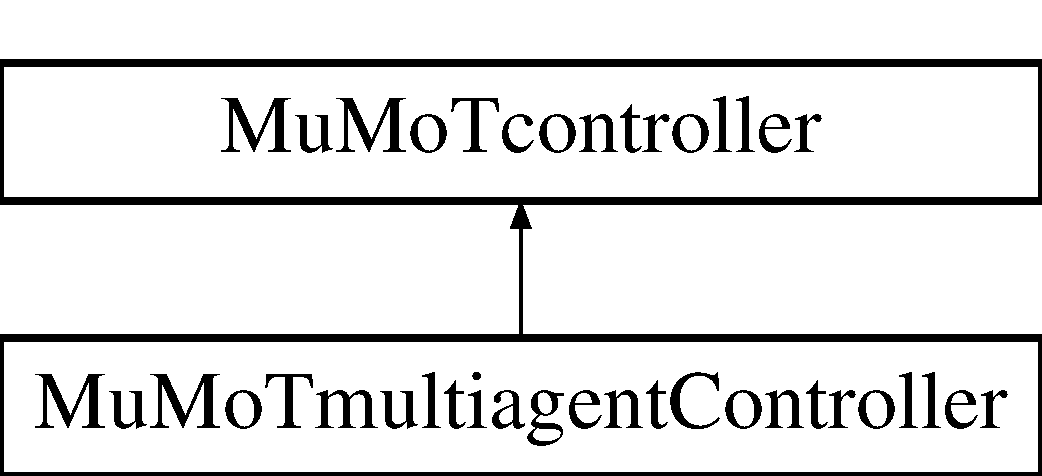
\includegraphics[height=2.000000cm]{class_mu_mo_t_1_1_mu_mo_tmultiagent_controller}
\end{center}
\end{figure}
\subsection*{Public Member Functions}
\begin{DoxyCompactItemize}
\item 
def \hyperlink{class_mu_mo_t_1_1_mu_mo_tmultiagent_controller_a203e76c007a565312c5715712851aadb}{\+\_\+\+\_\+init\+\_\+\+\_\+} (self, param\+Values, param\+Names, param\+Label\+Dict, continuous\+Replot, special\+Params)
\item 
def \hyperlink{class_mu_mo_t_1_1_mu_mo_tmultiagent_controller_afa43c0f74ab5a6630a4b7ab0af8ed990}{download\+Time\+Evolution} (self)
\end{DoxyCompactItemize}
\subsection*{Private Member Functions}
\begin{DoxyCompactItemize}
\item 
def \hyperlink{class_mu_mo_t_1_1_mu_mo_tmultiagent_controller_add4eacb8e812feeca1d4b2538e3bd6e0}{\+\_\+update\+\_\+params\+\_\+from\+\_\+widgets} (self)
\begin{DoxyCompactList}\small\item\em overwritten parent\textquotesingle{}s method. \end{DoxyCompactList}\item 
def \hyperlink{class_mu_mo_t_1_1_mu_mo_tmultiagent_controller_a05f01fc433f3ff6861ec56d6663cb84e}{\+\_\+update\+\_\+net\+\_\+params} (self)
\item 
def \hyperlink{class_mu_mo_t_1_1_mu_mo_tmultiagent_controller_a66b8497b0cb4b6a35c08c72da6ade6c3}{\+\_\+update\+\_\+scaling\+\_\+widget} (self, scaling)
\end{DoxyCompactItemize}
\subsection*{Private Attributes}
\begin{DoxyCompactItemize}
\item 
\hyperlink{class_mu_mo_t_1_1_mu_mo_tmultiagent_controller_a018864aa22d2adb0d3958fb0adbce8e2}{\+\_\+progress\+Bar}
\begin{DoxyCompactList}\small\item\em Network type dropdown selector. \end{DoxyCompactList}\end{DoxyCompactItemize}
\subsection*{Static Private Attributes}
\begin{DoxyCompactItemize}
\item 
\hyperlink{class_mu_mo_t_1_1_mu_mo_tmultiagent_controller_a559b8292a88eb343bf8591754cf168ef}{\+\_\+filetodownload} = None
\item 
\hyperlink{class_mu_mo_t_1_1_mu_mo_tmultiagent_controller_a8afeb8cf5705c6b521f7d6658dab955b}{\+\_\+initial\+State} = None
\end{DoxyCompactItemize}


\subsection{Detailed Description}
class describing a controller for multiagent views 

\subsection{Constructor \& Destructor Documentation}
\mbox{\Hypertarget{class_mu_mo_t_1_1_mu_mo_tmultiagent_controller_a203e76c007a565312c5715712851aadb}\label{class_mu_mo_t_1_1_mu_mo_tmultiagent_controller_a203e76c007a565312c5715712851aadb}} 
\index{Mu\+Mo\+T\+::\+Mu\+Mo\+Tmultiagent\+Controller@{Mu\+Mo\+T\+::\+Mu\+Mo\+Tmultiagent\+Controller}!\+\_\+\+\_\+init\+\_\+\+\_\+@{\+\_\+\+\_\+init\+\_\+\+\_\+}}
\index{\+\_\+\+\_\+init\+\_\+\+\_\+@{\+\_\+\+\_\+init\+\_\+\+\_\+}!Mu\+Mo\+T\+::\+Mu\+Mo\+Tmultiagent\+Controller@{Mu\+Mo\+T\+::\+Mu\+Mo\+Tmultiagent\+Controller}}
\subsubsection{\texorpdfstring{\+\_\+\+\_\+init\+\_\+\+\_\+()}{\_\_init\_\_()}}
{\footnotesize\ttfamily def \+\_\+\+\_\+init\+\_\+\+\_\+ (\begin{DoxyParamCaption}\item[{}]{self,  }\item[{}]{param\+Values,  }\item[{}]{param\+Names,  }\item[{}]{param\+Label\+Dict,  }\item[{}]{continuous\+Replot,  }\item[{}]{special\+Params }\end{DoxyParamCaption})}



\subsection{Member Function Documentation}
\mbox{\Hypertarget{class_mu_mo_t_1_1_mu_mo_tmultiagent_controller_a05f01fc433f3ff6861ec56d6663cb84e}\label{class_mu_mo_t_1_1_mu_mo_tmultiagent_controller_a05f01fc433f3ff6861ec56d6663cb84e}} 
\index{Mu\+Mo\+T\+::\+Mu\+Mo\+Tmultiagent\+Controller@{Mu\+Mo\+T\+::\+Mu\+Mo\+Tmultiagent\+Controller}!\+\_\+update\+\_\+net\+\_\+params@{\+\_\+update\+\_\+net\+\_\+params}}
\index{\+\_\+update\+\_\+net\+\_\+params@{\+\_\+update\+\_\+net\+\_\+params}!Mu\+Mo\+T\+::\+Mu\+Mo\+Tmultiagent\+Controller@{Mu\+Mo\+T\+::\+Mu\+Mo\+Tmultiagent\+Controller}}
\subsubsection{\texorpdfstring{\+\_\+update\+\_\+net\+\_\+params()}{\_update\_net\_params()}}
{\footnotesize\ttfamily def \+\_\+update\+\_\+net\+\_\+params (\begin{DoxyParamCaption}\item[{}]{self }\end{DoxyParamCaption})\hspace{0.3cm}{\ttfamily [private]}}

\mbox{\Hypertarget{class_mu_mo_t_1_1_mu_mo_tmultiagent_controller_add4eacb8e812feeca1d4b2538e3bd6e0}\label{class_mu_mo_t_1_1_mu_mo_tmultiagent_controller_add4eacb8e812feeca1d4b2538e3bd6e0}} 
\index{Mu\+Mo\+T\+::\+Mu\+Mo\+Tmultiagent\+Controller@{Mu\+Mo\+T\+::\+Mu\+Mo\+Tmultiagent\+Controller}!\+\_\+update\+\_\+params\+\_\+from\+\_\+widgets@{\+\_\+update\+\_\+params\+\_\+from\+\_\+widgets}}
\index{\+\_\+update\+\_\+params\+\_\+from\+\_\+widgets@{\+\_\+update\+\_\+params\+\_\+from\+\_\+widgets}!Mu\+Mo\+T\+::\+Mu\+Mo\+Tmultiagent\+Controller@{Mu\+Mo\+T\+::\+Mu\+Mo\+Tmultiagent\+Controller}}
\subsubsection{\texorpdfstring{\+\_\+update\+\_\+params\+\_\+from\+\_\+widgets()}{\_update\_params\_from\_widgets()}}
{\footnotesize\ttfamily def \+\_\+update\+\_\+params\+\_\+from\+\_\+widgets (\begin{DoxyParamCaption}\item[{}]{self }\end{DoxyParamCaption})\hspace{0.3cm}{\ttfamily [private]}}



overwritten parent\textquotesingle{}s method. 

Old method is not used becuase substituted by widget\+Dict \mbox{\Hypertarget{class_mu_mo_t_1_1_mu_mo_tmultiagent_controller_a66b8497b0cb4b6a35c08c72da6ade6c3}\label{class_mu_mo_t_1_1_mu_mo_tmultiagent_controller_a66b8497b0cb4b6a35c08c72da6ade6c3}} 
\index{Mu\+Mo\+T\+::\+Mu\+Mo\+Tmultiagent\+Controller@{Mu\+Mo\+T\+::\+Mu\+Mo\+Tmultiagent\+Controller}!\+\_\+update\+\_\+scaling\+\_\+widget@{\+\_\+update\+\_\+scaling\+\_\+widget}}
\index{\+\_\+update\+\_\+scaling\+\_\+widget@{\+\_\+update\+\_\+scaling\+\_\+widget}!Mu\+Mo\+T\+::\+Mu\+Mo\+Tmultiagent\+Controller@{Mu\+Mo\+T\+::\+Mu\+Mo\+Tmultiagent\+Controller}}
\subsubsection{\texorpdfstring{\+\_\+update\+\_\+scaling\+\_\+widget()}{\_update\_scaling\_widget()}}
{\footnotesize\ttfamily def \+\_\+update\+\_\+scaling\+\_\+widget (\begin{DoxyParamCaption}\item[{}]{self,  }\item[{}]{scaling }\end{DoxyParamCaption})\hspace{0.3cm}{\ttfamily [private]}}

\mbox{\Hypertarget{class_mu_mo_t_1_1_mu_mo_tmultiagent_controller_afa43c0f74ab5a6630a4b7ab0af8ed990}\label{class_mu_mo_t_1_1_mu_mo_tmultiagent_controller_afa43c0f74ab5a6630a4b7ab0af8ed990}} 
\index{Mu\+Mo\+T\+::\+Mu\+Mo\+Tmultiagent\+Controller@{Mu\+Mo\+T\+::\+Mu\+Mo\+Tmultiagent\+Controller}!download\+Time\+Evolution@{download\+Time\+Evolution}}
\index{download\+Time\+Evolution@{download\+Time\+Evolution}!Mu\+Mo\+T\+::\+Mu\+Mo\+Tmultiagent\+Controller@{Mu\+Mo\+T\+::\+Mu\+Mo\+Tmultiagent\+Controller}}
\subsubsection{\texorpdfstring{download\+Time\+Evolution()}{downloadTimeEvolution()}}
{\footnotesize\ttfamily def download\+Time\+Evolution (\begin{DoxyParamCaption}\item[{}]{self }\end{DoxyParamCaption})}



\subsection{Field Documentation}
\mbox{\Hypertarget{class_mu_mo_t_1_1_mu_mo_tmultiagent_controller_a559b8292a88eb343bf8591754cf168ef}\label{class_mu_mo_t_1_1_mu_mo_tmultiagent_controller_a559b8292a88eb343bf8591754cf168ef}} 
\index{Mu\+Mo\+T\+::\+Mu\+Mo\+Tmultiagent\+Controller@{Mu\+Mo\+T\+::\+Mu\+Mo\+Tmultiagent\+Controller}!\+\_\+filetodownload@{\+\_\+filetodownload}}
\index{\+\_\+filetodownload@{\+\_\+filetodownload}!Mu\+Mo\+T\+::\+Mu\+Mo\+Tmultiagent\+Controller@{Mu\+Mo\+T\+::\+Mu\+Mo\+Tmultiagent\+Controller}}
\subsubsection{\texorpdfstring{\+\_\+filetodownload}{\_filetodownload}}
{\footnotesize\ttfamily \+\_\+filetodownload = None\hspace{0.3cm}{\ttfamily [static]}, {\ttfamily [private]}}

\mbox{\Hypertarget{class_mu_mo_t_1_1_mu_mo_tmultiagent_controller_a8afeb8cf5705c6b521f7d6658dab955b}\label{class_mu_mo_t_1_1_mu_mo_tmultiagent_controller_a8afeb8cf5705c6b521f7d6658dab955b}} 
\index{Mu\+Mo\+T\+::\+Mu\+Mo\+Tmultiagent\+Controller@{Mu\+Mo\+T\+::\+Mu\+Mo\+Tmultiagent\+Controller}!\+\_\+initial\+State@{\+\_\+initial\+State}}
\index{\+\_\+initial\+State@{\+\_\+initial\+State}!Mu\+Mo\+T\+::\+Mu\+Mo\+Tmultiagent\+Controller@{Mu\+Mo\+T\+::\+Mu\+Mo\+Tmultiagent\+Controller}}
\subsubsection{\texorpdfstring{\+\_\+initial\+State}{\_initialState}}
{\footnotesize\ttfamily \+\_\+initial\+State = None\hspace{0.3cm}{\ttfamily [static]}, {\ttfamily [private]}}

\mbox{\Hypertarget{class_mu_mo_t_1_1_mu_mo_tmultiagent_controller_a018864aa22d2adb0d3958fb0adbce8e2}\label{class_mu_mo_t_1_1_mu_mo_tmultiagent_controller_a018864aa22d2adb0d3958fb0adbce8e2}} 
\index{Mu\+Mo\+T\+::\+Mu\+Mo\+Tmultiagent\+Controller@{Mu\+Mo\+T\+::\+Mu\+Mo\+Tmultiagent\+Controller}!\+\_\+progress\+Bar@{\+\_\+progress\+Bar}}
\index{\+\_\+progress\+Bar@{\+\_\+progress\+Bar}!Mu\+Mo\+T\+::\+Mu\+Mo\+Tmultiagent\+Controller@{Mu\+Mo\+T\+::\+Mu\+Mo\+Tmultiagent\+Controller}}
\subsubsection{\texorpdfstring{\+\_\+progress\+Bar}{\_progressBar}}
{\footnotesize\ttfamily \+\_\+progress\+Bar\hspace{0.3cm}{\ttfamily [private]}}



Network type dropdown selector. 

\begin{DoxyRefDesc}{Todo}
\item[\hyperlink{todo__todo000020}{Todo}]\+: add network topology generated by random points in space \end{DoxyRefDesc}
Toggle buttons for plotting style 

The documentation for this class was generated from the following file\+:\begin{DoxyCompactItemize}
\item 
\hyperlink{_mu_mo_t_8py}{Mu\+Mo\+T.\+py}\end{DoxyCompactItemize}

\hypertarget{class_mu_mo_t_1_1_mu_mo_tnetwork_view}{}\section{Mu\+Mo\+Tnetwork\+View Class Reference}
\label{class_mu_mo_t_1_1_mu_mo_tnetwork_view}\index{Mu\+Mo\+Tnetwork\+View@{Mu\+Mo\+Tnetwork\+View}}


self.\+\_\+py\+D\+Scont.\+new\+Curve(self.\+\_\+py\+D\+Scont\+Args) self.\+\_\+py\+D\+Scont\mbox{[}\textquotesingle{}E\+Q1\textquotesingle{}\mbox{]}.reset(self.\+\_\+py\+D\+Smodel.\+pars) self.\+\_\+py\+D\+Sode.\+set(pars = self.\+\_\+py\+D\+Smodel.\+pars) self.\+\_\+py\+D\+Scont\mbox{[}\textquotesingle{}E\+Q1\textquotesingle{}\mbox{]}.reset() self.\+\_\+py\+D\+Scont.\+update(self.\+\_\+py\+D\+Scont\+Args) \# T\+O\+DO\+: what does this do?  


Inheritance diagram for Mu\+Mo\+Tnetwork\+View\+:\begin{figure}[H]
\begin{center}
\leavevmode
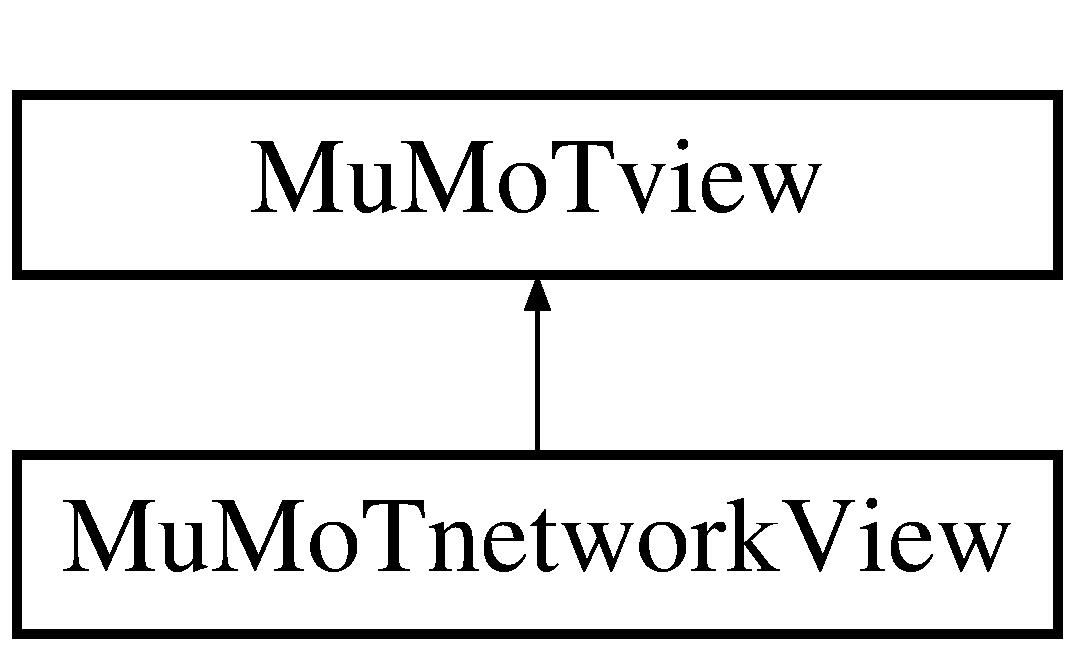
\includegraphics[height=2.000000cm]{class_mu_mo_t_1_1_mu_mo_tnetwork_view}
\end{center}
\end{figure}


\subsection{Detailed Description}
self.\+\_\+py\+D\+Scont.\+new\+Curve(self.\+\_\+py\+D\+Scont\+Args) self.\+\_\+py\+D\+Scont\mbox{[}\textquotesingle{}E\+Q1\textquotesingle{}\mbox{]}.reset(self.\+\_\+py\+D\+Smodel.\+pars) self.\+\_\+py\+D\+Sode.\+set(pars = self.\+\_\+py\+D\+Smodel.\+pars) self.\+\_\+py\+D\+Scont\mbox{[}\textquotesingle{}E\+Q1\textquotesingle{}\mbox{]}.reset() self.\+\_\+py\+D\+Scont.\+update(self.\+\_\+py\+D\+Scont\+Args) \# T\+O\+DO\+: what does this do? 

The documentation for this class was generated from the following file\+:\begin{DoxyCompactItemize}
\item 
/\+Users/marshall/\+Google Drive/\+Home/\+Git/\+Mu\+Mo\+T/Mu\+Mo\+T.\+py\end{DoxyCompactItemize}

\hypertarget{class_mu_mo_t_1_1_mu_mo_tstream_view}{}\section{Mu\+Mo\+Tstream\+View Class Reference}
\label{class_mu_mo_t_1_1_mu_mo_tstream_view}\index{Mu\+Mo\+Tstream\+View@{Mu\+Mo\+Tstream\+View}}
Inheritance diagram for Mu\+Mo\+Tstream\+View\+:\begin{figure}[H]
\begin{center}
\leavevmode
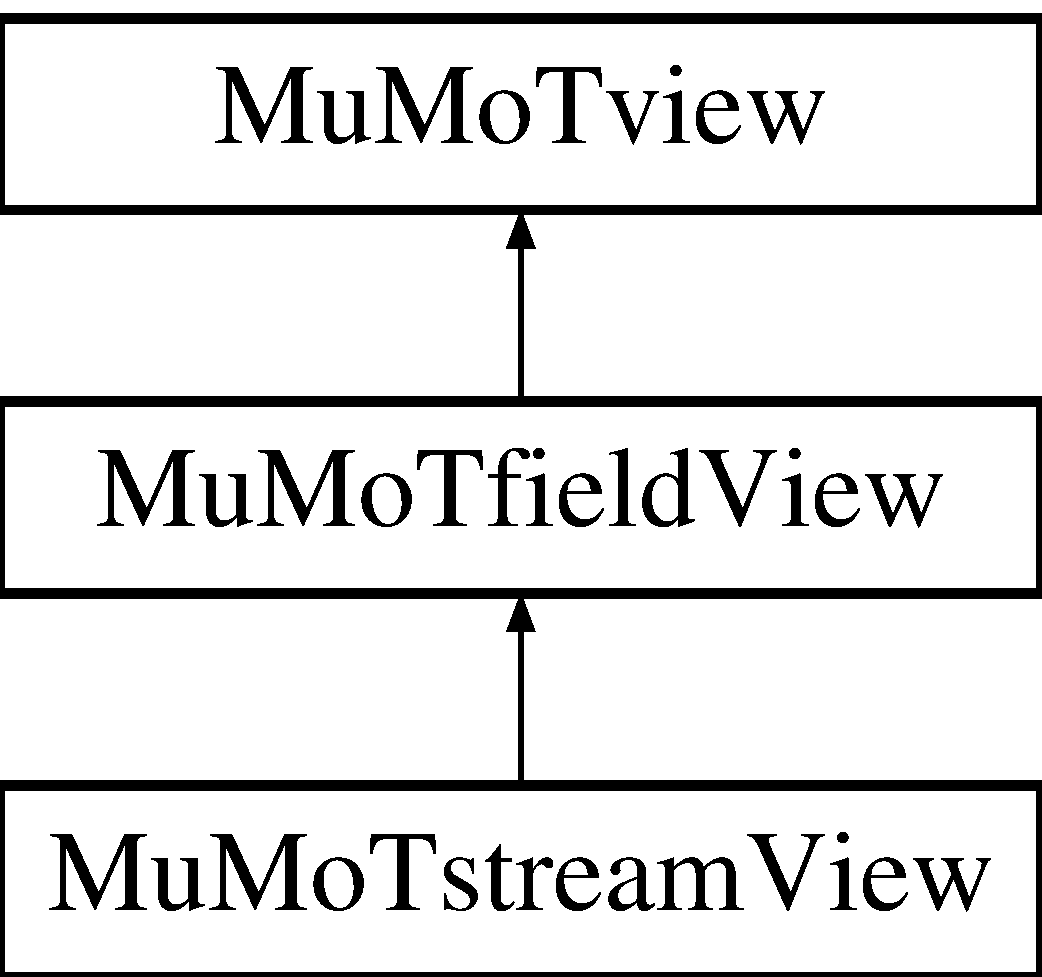
\includegraphics[height=3.000000cm]{class_mu_mo_t_1_1_mu_mo_tstream_view}
\end{center}
\end{figure}
\subsection*{Private Member Functions}
\begin{DoxyCompactItemize}
\item 
def \hyperlink{class_mu_mo_t_1_1_mu_mo_tstream_view_a50d59419298116f738a98c864afb9d89}{\+\_\+plot\+\_\+field} (self)
\end{DoxyCompactItemize}


\subsection{Member Function Documentation}
\mbox{\Hypertarget{class_mu_mo_t_1_1_mu_mo_tstream_view_a50d59419298116f738a98c864afb9d89}\label{class_mu_mo_t_1_1_mu_mo_tstream_view_a50d59419298116f738a98c864afb9d89}} 
\index{Mu\+Mo\+T\+::\+Mu\+Mo\+Tstream\+View@{Mu\+Mo\+T\+::\+Mu\+Mo\+Tstream\+View}!\+\_\+plot\+\_\+field@{\+\_\+plot\+\_\+field}}
\index{\+\_\+plot\+\_\+field@{\+\_\+plot\+\_\+field}!Mu\+Mo\+T\+::\+Mu\+Mo\+Tstream\+View@{Mu\+Mo\+T\+::\+Mu\+Mo\+Tstream\+View}}
\subsubsection{\texorpdfstring{\+\_\+plot\+\_\+field()}{\_plot\_field()}}
{\footnotesize\ttfamily def \+\_\+plot\+\_\+field (\begin{DoxyParamCaption}\item[{}]{self }\end{DoxyParamCaption})\hspace{0.3cm}{\ttfamily [private]}}



The documentation for this class was generated from the following file\+:\begin{DoxyCompactItemize}
\item 
\hyperlink{_mu_mo_t_8py}{Mu\+Mo\+T.\+py}\end{DoxyCompactItemize}

\hypertarget{class_mu_mo_t_1_1_mu_mo_tvector_view}{}\section{Mu\+Mo\+Tvector\+View Class Reference}
\label{class_mu_mo_t_1_1_mu_mo_tvector_view}\index{Mu\+Mo\+Tvector\+View@{Mu\+Mo\+Tvector\+View}}


vector plot view on model  


Inheritance diagram for Mu\+Mo\+Tvector\+View\+:\begin{figure}[H]
\begin{center}
\leavevmode
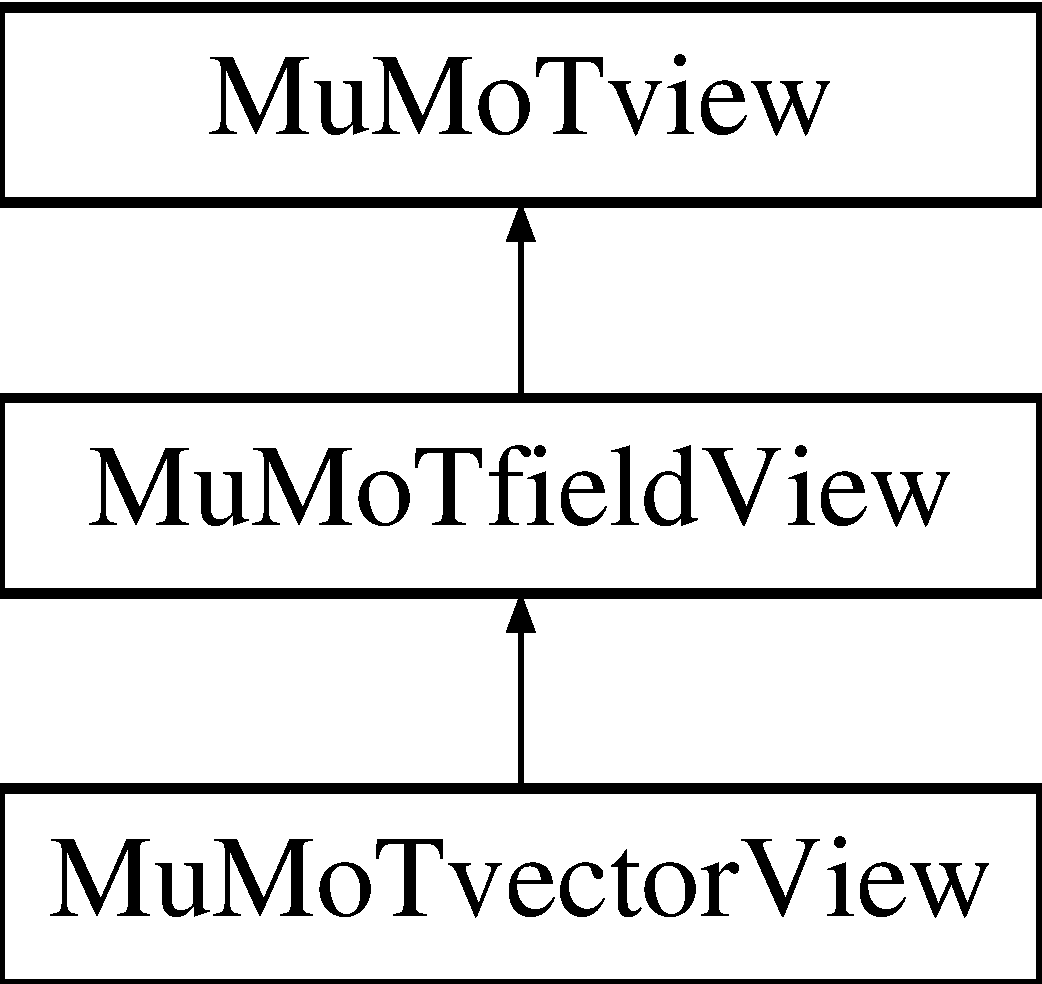
\includegraphics[height=3.000000cm]{class_mu_mo_t_1_1_mu_mo_tvector_view}
\end{center}
\end{figure}
\subsection*{Static Public Attributes}
\begin{DoxyCompactItemize}
\item 
\hyperlink{class_mu_mo_t_1_1_mu_mo_tvector_view_a8fa675eb2fcec5b95d9d21c670da7f30}{ax} = self.\+\_\+figure.\+gca(projection = \textquotesingle{}3d\textquotesingle{})
\item 
\hyperlink{class_mu_mo_t_1_1_mu_mo_tvector_view_a0d21a210e4f523569e4c57a12f80040c}{fig\+\_\+vec3d} = ax.\+quiver(self.\+\_\+X, self.\+\_\+Y, self.\+\_\+Z, self.\+\_\+\+Xdot, self.\+\_\+\+Ydot, self.\+\_\+\+Zdot, length = 0.\+01, \hyperlink{class_mu_mo_t_1_1_mu_mo_tview_a37dbdc30935031c05304482e1be89d8f}{color} = \textquotesingle{}black\textquotesingle{})
\item 
\hyperlink{class_mu_mo_t_1_1_mu_mo_tvector_view_abb76a7390100209788848dbd6bb9fe30}{xlab}
\item 
\hyperlink{class_mu_mo_t_1_1_mu_mo_tvector_view_a83433d4e45c13afe9a0042ae113ad169}{ylab}
\item 
\hyperlink{class_mu_mo_t_1_1_mu_mo_tvector_view_a180fbd5bd60d175c88a69e1dd3b0ed77}{zlab}
\item 
\hyperlink{class_mu_mo_t_1_1_mu_mo_tvector_view_a73c8f7f0d9593ed55a0cb1bea896b9f4}{ax\+\_\+reformat}
\item 
\hyperlink{class_mu_mo_t_1_1_mu_mo_tvector_view_a643a20c0c59588a0f741a6095e2025fd}{True}
\item 
\hyperlink{class_mu_mo_t_1_1_mu_mo_tvector_view_a44c38482b3d22d05f8bbadb81ec2d40a}{show\+Plane}
\end{DoxyCompactItemize}
\subsection*{Private Member Functions}
\begin{DoxyCompactItemize}
\item 
def \hyperlink{class_mu_mo_t_1_1_mu_mo_tvector_view_a50d59419298116f738a98c864afb9d89}{\+\_\+plot\+\_\+field} (self)
\end{DoxyCompactItemize}
\subsection*{Private Attributes}
\begin{DoxyCompactItemize}
\item 
\hyperlink{class_mu_mo_t_1_1_mu_mo_tvector_view_ad2f8dc44173a16468bd9d3ab335f9b27}{\+\_\+state\+Variable3}
\end{DoxyCompactItemize}
\subsection*{Static Private Attributes}
\begin{DoxyCompactItemize}
\item 
\hyperlink{class_mu_mo_t_1_1_mu_mo_tvector_view_a865b2109ba10d874e84d4a354873b121}{\+\_\+xlab}
\item 
\hyperlink{class_mu_mo_t_1_1_mu_mo_tvector_view_aac1a25a634d53e524573f67eb5f3a7b9}{\+\_\+ylab}
\end{DoxyCompactItemize}
\subsection*{Additional Inherited Members}


\subsection{Detailed Description}
vector plot view on model 

\subsection{Member Function Documentation}
\mbox{\Hypertarget{class_mu_mo_t_1_1_mu_mo_tvector_view_a50d59419298116f738a98c864afb9d89}\label{class_mu_mo_t_1_1_mu_mo_tvector_view_a50d59419298116f738a98c864afb9d89}} 
\index{Mu\+Mo\+T\+::\+Mu\+Mo\+Tvector\+View@{Mu\+Mo\+T\+::\+Mu\+Mo\+Tvector\+View}!\+\_\+plot\+\_\+field@{\+\_\+plot\+\_\+field}}
\index{\+\_\+plot\+\_\+field@{\+\_\+plot\+\_\+field}!Mu\+Mo\+T\+::\+Mu\+Mo\+Tvector\+View@{Mu\+Mo\+T\+::\+Mu\+Mo\+Tvector\+View}}
\subsubsection{\texorpdfstring{\+\_\+plot\+\_\+field()}{\_plot\_field()}}
{\footnotesize\ttfamily def \+\_\+plot\+\_\+field (\begin{DoxyParamCaption}\item[{}]{self }\end{DoxyParamCaption})\hspace{0.3cm}{\ttfamily [private]}}



\subsection{Field Documentation}
\mbox{\Hypertarget{class_mu_mo_t_1_1_mu_mo_tvector_view_ad2f8dc44173a16468bd9d3ab335f9b27}\label{class_mu_mo_t_1_1_mu_mo_tvector_view_ad2f8dc44173a16468bd9d3ab335f9b27}} 
\index{Mu\+Mo\+T\+::\+Mu\+Mo\+Tvector\+View@{Mu\+Mo\+T\+::\+Mu\+Mo\+Tvector\+View}!\+\_\+state\+Variable3@{\+\_\+state\+Variable3}}
\index{\+\_\+state\+Variable3@{\+\_\+state\+Variable3}!Mu\+Mo\+T\+::\+Mu\+Mo\+Tvector\+View@{Mu\+Mo\+T\+::\+Mu\+Mo\+Tvector\+View}}
\subsubsection{\texorpdfstring{\+\_\+state\+Variable3}{\_stateVariable3}}
{\footnotesize\ttfamily \+\_\+state\+Variable3\hspace{0.3cm}{\ttfamily [private]}}

\mbox{\Hypertarget{class_mu_mo_t_1_1_mu_mo_tvector_view_a865b2109ba10d874e84d4a354873b121}\label{class_mu_mo_t_1_1_mu_mo_tvector_view_a865b2109ba10d874e84d4a354873b121}} 
\index{Mu\+Mo\+T\+::\+Mu\+Mo\+Tvector\+View@{Mu\+Mo\+T\+::\+Mu\+Mo\+Tvector\+View}!\+\_\+xlab@{\+\_\+xlab}}
\index{\+\_\+xlab@{\+\_\+xlab}!Mu\+Mo\+T\+::\+Mu\+Mo\+Tvector\+View@{Mu\+Mo\+T\+::\+Mu\+Mo\+Tvector\+View}}
\subsubsection{\texorpdfstring{\+\_\+xlab}{\_xlab}}
{\footnotesize\ttfamily \+\_\+xlab\hspace{0.3cm}{\ttfamily [static]}, {\ttfamily [private]}}

\mbox{\Hypertarget{class_mu_mo_t_1_1_mu_mo_tvector_view_aac1a25a634d53e524573f67eb5f3a7b9}\label{class_mu_mo_t_1_1_mu_mo_tvector_view_aac1a25a634d53e524573f67eb5f3a7b9}} 
\index{Mu\+Mo\+T\+::\+Mu\+Mo\+Tvector\+View@{Mu\+Mo\+T\+::\+Mu\+Mo\+Tvector\+View}!\+\_\+ylab@{\+\_\+ylab}}
\index{\+\_\+ylab@{\+\_\+ylab}!Mu\+Mo\+T\+::\+Mu\+Mo\+Tvector\+View@{Mu\+Mo\+T\+::\+Mu\+Mo\+Tvector\+View}}
\subsubsection{\texorpdfstring{\+\_\+ylab}{\_ylab}}
{\footnotesize\ttfamily \+\_\+ylab\hspace{0.3cm}{\ttfamily [static]}, {\ttfamily [private]}}

\mbox{\Hypertarget{class_mu_mo_t_1_1_mu_mo_tvector_view_a8fa675eb2fcec5b95d9d21c670da7f30}\label{class_mu_mo_t_1_1_mu_mo_tvector_view_a8fa675eb2fcec5b95d9d21c670da7f30}} 
\index{Mu\+Mo\+T\+::\+Mu\+Mo\+Tvector\+View@{Mu\+Mo\+T\+::\+Mu\+Mo\+Tvector\+View}!ax@{ax}}
\index{ax@{ax}!Mu\+Mo\+T\+::\+Mu\+Mo\+Tvector\+View@{Mu\+Mo\+T\+::\+Mu\+Mo\+Tvector\+View}}
\subsubsection{\texorpdfstring{ax}{ax}}
{\footnotesize\ttfamily ax = self.\+\_\+figure.\+gca(projection = \textquotesingle{}3d\textquotesingle{})\hspace{0.3cm}{\ttfamily [static]}}

\mbox{\Hypertarget{class_mu_mo_t_1_1_mu_mo_tvector_view_a73c8f7f0d9593ed55a0cb1bea896b9f4}\label{class_mu_mo_t_1_1_mu_mo_tvector_view_a73c8f7f0d9593ed55a0cb1bea896b9f4}} 
\index{Mu\+Mo\+T\+::\+Mu\+Mo\+Tvector\+View@{Mu\+Mo\+T\+::\+Mu\+Mo\+Tvector\+View}!ax\+\_\+reformat@{ax\+\_\+reformat}}
\index{ax\+\_\+reformat@{ax\+\_\+reformat}!Mu\+Mo\+T\+::\+Mu\+Mo\+Tvector\+View@{Mu\+Mo\+T\+::\+Mu\+Mo\+Tvector\+View}}
\subsubsection{\texorpdfstring{ax\+\_\+reformat}{ax\_reformat}}
{\footnotesize\ttfamily ax\+\_\+reformat\hspace{0.3cm}{\ttfamily [static]}}

\mbox{\Hypertarget{class_mu_mo_t_1_1_mu_mo_tvector_view_a0d21a210e4f523569e4c57a12f80040c}\label{class_mu_mo_t_1_1_mu_mo_tvector_view_a0d21a210e4f523569e4c57a12f80040c}} 
\index{Mu\+Mo\+T\+::\+Mu\+Mo\+Tvector\+View@{Mu\+Mo\+T\+::\+Mu\+Mo\+Tvector\+View}!fig\+\_\+vec3d@{fig\+\_\+vec3d}}
\index{fig\+\_\+vec3d@{fig\+\_\+vec3d}!Mu\+Mo\+T\+::\+Mu\+Mo\+Tvector\+View@{Mu\+Mo\+T\+::\+Mu\+Mo\+Tvector\+View}}
\subsubsection{\texorpdfstring{fig\+\_\+vec3d}{fig\_vec3d}}
{\footnotesize\ttfamily fig\+\_\+vec3d = ax.\+quiver(self.\+\_\+X, self.\+\_\+Y, self.\+\_\+Z, self.\+\_\+\+Xdot, self.\+\_\+\+Ydot, self.\+\_\+\+Zdot, length = 0.\+01, \hyperlink{class_mu_mo_t_1_1_mu_mo_tview_a37dbdc30935031c05304482e1be89d8f}{color} = \textquotesingle{}black\textquotesingle{})\hspace{0.3cm}{\ttfamily [static]}}

\mbox{\Hypertarget{class_mu_mo_t_1_1_mu_mo_tvector_view_a44c38482b3d22d05f8bbadb81ec2d40a}\label{class_mu_mo_t_1_1_mu_mo_tvector_view_a44c38482b3d22d05f8bbadb81ec2d40a}} 
\index{Mu\+Mo\+T\+::\+Mu\+Mo\+Tvector\+View@{Mu\+Mo\+T\+::\+Mu\+Mo\+Tvector\+View}!show\+Plane@{show\+Plane}}
\index{show\+Plane@{show\+Plane}!Mu\+Mo\+T\+::\+Mu\+Mo\+Tvector\+View@{Mu\+Mo\+T\+::\+Mu\+Mo\+Tvector\+View}}
\subsubsection{\texorpdfstring{show\+Plane}{showPlane}}
{\footnotesize\ttfamily show\+Plane\hspace{0.3cm}{\ttfamily [static]}}

\mbox{\Hypertarget{class_mu_mo_t_1_1_mu_mo_tvector_view_a643a20c0c59588a0f741a6095e2025fd}\label{class_mu_mo_t_1_1_mu_mo_tvector_view_a643a20c0c59588a0f741a6095e2025fd}} 
\index{Mu\+Mo\+T\+::\+Mu\+Mo\+Tvector\+View@{Mu\+Mo\+T\+::\+Mu\+Mo\+Tvector\+View}!True@{True}}
\index{True@{True}!Mu\+Mo\+T\+::\+Mu\+Mo\+Tvector\+View@{Mu\+Mo\+T\+::\+Mu\+Mo\+Tvector\+View}}
\subsubsection{\texorpdfstring{True}{True}}
{\footnotesize\ttfamily True\hspace{0.3cm}{\ttfamily [static]}}

\mbox{\Hypertarget{class_mu_mo_t_1_1_mu_mo_tvector_view_abb76a7390100209788848dbd6bb9fe30}\label{class_mu_mo_t_1_1_mu_mo_tvector_view_abb76a7390100209788848dbd6bb9fe30}} 
\index{Mu\+Mo\+T\+::\+Mu\+Mo\+Tvector\+View@{Mu\+Mo\+T\+::\+Mu\+Mo\+Tvector\+View}!xlab@{xlab}}
\index{xlab@{xlab}!Mu\+Mo\+T\+::\+Mu\+Mo\+Tvector\+View@{Mu\+Mo\+T\+::\+Mu\+Mo\+Tvector\+View}}
\subsubsection{\texorpdfstring{xlab}{xlab}}
{\footnotesize\ttfamily xlab\hspace{0.3cm}{\ttfamily [static]}}

\mbox{\Hypertarget{class_mu_mo_t_1_1_mu_mo_tvector_view_a83433d4e45c13afe9a0042ae113ad169}\label{class_mu_mo_t_1_1_mu_mo_tvector_view_a83433d4e45c13afe9a0042ae113ad169}} 
\index{Mu\+Mo\+T\+::\+Mu\+Mo\+Tvector\+View@{Mu\+Mo\+T\+::\+Mu\+Mo\+Tvector\+View}!ylab@{ylab}}
\index{ylab@{ylab}!Mu\+Mo\+T\+::\+Mu\+Mo\+Tvector\+View@{Mu\+Mo\+T\+::\+Mu\+Mo\+Tvector\+View}}
\subsubsection{\texorpdfstring{ylab}{ylab}}
{\footnotesize\ttfamily ylab\hspace{0.3cm}{\ttfamily [static]}}

\mbox{\Hypertarget{class_mu_mo_t_1_1_mu_mo_tvector_view_a180fbd5bd60d175c88a69e1dd3b0ed77}\label{class_mu_mo_t_1_1_mu_mo_tvector_view_a180fbd5bd60d175c88a69e1dd3b0ed77}} 
\index{Mu\+Mo\+T\+::\+Mu\+Mo\+Tvector\+View@{Mu\+Mo\+T\+::\+Mu\+Mo\+Tvector\+View}!zlab@{zlab}}
\index{zlab@{zlab}!Mu\+Mo\+T\+::\+Mu\+Mo\+Tvector\+View@{Mu\+Mo\+T\+::\+Mu\+Mo\+Tvector\+View}}
\subsubsection{\texorpdfstring{zlab}{zlab}}
{\footnotesize\ttfamily zlab\hspace{0.3cm}{\ttfamily [static]}}



The documentation for this class was generated from the following file\+:\begin{DoxyCompactItemize}
\item 
\hyperlink{_mu_mo_t_8py}{Mu\+Mo\+T.\+py}\end{DoxyCompactItemize}

\hypertarget{class_mu_mo_t_1_1_mu_mo_tview}{}\section{Mu\+Mo\+Tview Class Reference}
\label{class_mu_mo_t_1_1_mu_mo_tview}\index{Mu\+Mo\+Tview@{Mu\+Mo\+Tview}}


class describing a view on a model  


Inheritance diagram for Mu\+Mo\+Tview\+:\begin{figure}[H]
\begin{center}
\leavevmode
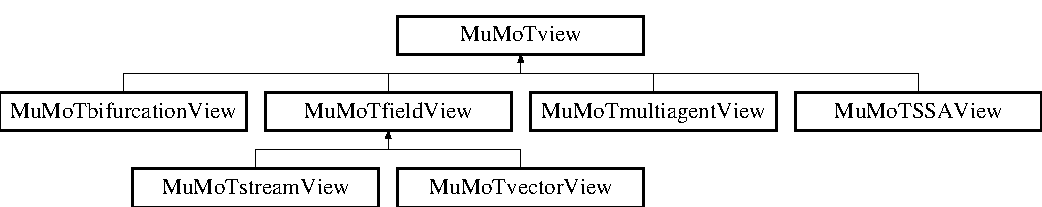
\includegraphics[height=2.225166cm]{class_mu_mo_t_1_1_mu_mo_tview}
\end{center}
\end{figure}
\subsection*{Public Member Functions}
\begin{DoxyCompactItemize}
\item 
def \hyperlink{class_mu_mo_t_1_1_mu_mo_tview_a367325b3bd7ca4a7b7ec4107f9aa6a16}{\+\_\+\+\_\+init\+\_\+\+\_\+} (self, model, controller, figure=None, params=None, kwargs)
\item 
def \hyperlink{class_mu_mo_t_1_1_mu_mo_tview_aca4d648d909f4722c7e07197675500bb}{show\+Logs} (self)
\end{DoxyCompactItemize}
\subsection*{Static Public Attributes}
\begin{DoxyCompactItemize}
\item 
\hyperlink{class_mu_mo_t_1_1_mu_mo_tview_afcc7a4b78ecd8fa7e713f8cfa0f51017}{value}
\item 
\hyperlink{class_mu_mo_t_1_1_mu_mo_tview_a2661f439a4a94ffdcd5e47ae1da0bb1d}{description}
\item 
\hyperlink{class_mu_mo_t_1_1_mu_mo_tview_a37d874d1d45bc2e5bfa013cddacb8e68}{logs} = self.\+\_\+single\+Run(random\+Seeds\mbox{[}i\mbox{]})
\item 
\hyperlink{class_mu_mo_t_1_1_mu_mo_tview_a69ffe654c8e97fdcbffcf35a1ded8157}{system\+Size} = sum(self.\+\_\+controller.\+\_\+initial\+State.\+values())
\begin{DoxyCompactList}\small\item\em Plot. \end{DoxyCompactList}\item 
\hyperlink{class_mu_mo_t_1_1_mu_mo_tview_aa820f7e11b025b06f4eeb0ad7581ad34}{max\+Time} = self.\+\_\+controller.\+\_\+widget\+Dict\mbox{[}\textquotesingle{}max\+Time\textquotesingle{}\mbox{]}.\hyperlink{class_mu_mo_t_1_1_mu_mo_tview_afcc7a4b78ecd8fa7e713f8cfa0f51017}{value}
\item 
\hyperlink{class_mu_mo_t_1_1_mu_mo_tview_a23acc33d21869c517c7eb8114b3d8072}{pop}
\item 
\hyperlink{class_mu_mo_t_1_1_mu_mo_tview_a37dbdc30935031c05304482e1be89d8f}{color}
\item 
list \hyperlink{class_mu_mo_t_1_1_mu_mo_tview_a6a57a88c0fcb681f5721c6b1bce2dd96}{markers} = \mbox{[}plt.\+Line2D(\mbox{[}0,0\mbox{]},\mbox{[}0,0\mbox{]},\hyperlink{class_mu_mo_t_1_1_mu_mo_tview_a37dbdc30935031c05304482e1be89d8f}{color}=\hyperlink{class_mu_mo_t_1_1_mu_mo_tview_a37dbdc30935031c05304482e1be89d8f}{color}, marker=\textquotesingle{}\textquotesingle{}, linestyle=\textquotesingle{}-\/\textquotesingle{}) for \hyperlink{class_mu_mo_t_1_1_mu_mo_tview_a37dbdc30935031c05304482e1be89d8f}{color} in color\+Map.\+values()\mbox{]}
\item 
\hyperlink{class_mu_mo_t_1_1_mu_mo_tview_a411167eeca51189fabe03f884c7bf92c}{bbox\+\_\+to\+\_\+anchor}
\item 
\hyperlink{class_mu_mo_t_1_1_mu_mo_tview_aeee9f371db14fda0de35d16324a167df}{loc}
\item 
\hyperlink{class_mu_mo_t_1_1_mu_mo_tview_a15c45102c35a6e8e18adffce8cfdb703}{borderaxespad}
\end{DoxyCompactItemize}
\subsection*{Private Member Functions}
\begin{DoxyCompactItemize}
\item 
def \hyperlink{class_mu_mo_t_1_1_mu_mo_tview_a6822b561e2f9b618639714cd1545772e}{\+\_\+reset\+Error\+Message} (self)
\item 
def \hyperlink{class_mu_mo_t_1_1_mu_mo_tview_a23d2499d6c6334e35bc4cd7de3dd4d3c}{\+\_\+show\+Error\+Message} (self, message)
\item 
def \hyperlink{class_mu_mo_t_1_1_mu_mo_tview_abfc1e19ed53c088799d1f499bc010f7f}{\+\_\+set\+Log} (self, log)
\item 
def \hyperlink{class_mu_mo_t_1_1_mu_mo_tview_a8b4ffd0e4999bd45c6ca33fe0f40d1e3}{\+\_\+log} (self, analysis)
\item 
def \hyperlink{class_mu_mo_t_1_1_mu_mo_tview_a4d4a00545816bf68f912f5ea5a449c48}{\+\_\+multirun} (self, iterations, random\+Seeds)
\item 
def \hyperlink{class_mu_mo_t_1_1_mu_mo_tview_a51d421aacb4cd83af5f1c2e60c3dff9c}{\+\_\+single\+Run} (self, random\+Seed)
\begin{DoxyCompactList}\small\item\em overwrite this method for views that allow the \textquotesingle{}multirun\textquotesingle{} command \end{DoxyCompactList}\end{DoxyCompactItemize}
\subsection*{Static Private Attributes}
\begin{DoxyCompactItemize}
\item 
\hyperlink{class_mu_mo_t_1_1_mu_mo_tview_aeacd9541246371f0db5cc3e3779762fa}{\+\_\+mumot\+Model} = None
\begin{DoxyCompactList}\small\item\em Model view is on. \end{DoxyCompactList}\item 
\hyperlink{class_mu_mo_t_1_1_mu_mo_tview_abf6d9f6be3898e307415d4598cde264d}{\+\_\+figure} = None
\begin{DoxyCompactList}\small\item\em Figure/axis object to plot view to. \end{DoxyCompactList}\item 
\hyperlink{class_mu_mo_t_1_1_mu_mo_tview_a5748371a5f2e09033908d21bb12f94c0}{\+\_\+figure\+Num} = None
\begin{DoxyCompactList}\small\item\em Unique figure number. \end{DoxyCompactList}\item 
\hyperlink{class_mu_mo_t_1_1_mu_mo_tview_a506ccaeadc9c6f4102cf4e06f5a6be2a}{\+\_\+axes3d} = None
\begin{DoxyCompactList}\small\item\em 3d axes? (False =$>$ 2d) \end{DoxyCompactList}\item 
\hyperlink{class_mu_mo_t_1_1_mu_mo_tview_a15f56ca9811d1e67d721fa64f9b0dc1e}{\+\_\+controller} = None
\begin{DoxyCompactList}\small\item\em Controller that controls this view. \end{DoxyCompactList}\item 
\hyperlink{class_mu_mo_t_1_1_mu_mo_tview_ac0ad5d0ca27f2668c0676334ee73ff52}{\+\_\+logs} = None
\begin{DoxyCompactList}\small\item\em Summary logs of view behaviour. \end{DoxyCompactList}\item 
\hyperlink{class_mu_mo_t_1_1_mu_mo_tview_a5feff4ca83ee97d6e09874496a4975d4}{\+\_\+plot\+Type} = None
\begin{DoxyCompactList}\small\item\em Plotting method to use. \end{DoxyCompactList}\item 
\hyperlink{class_mu_mo_t_1_1_mu_mo_tview_ac7734326ac8dbbf9bd0d2c9838633195}{\+\_\+param\+Names} = None
\begin{DoxyCompactList}\small\item\em parameter names when used without controller \end{DoxyCompactList}\item 
\hyperlink{class_mu_mo_t_1_1_mu_mo_tview_a04608181fa27d9aad4983d3694f7ab17}{\+\_\+param\+Values} = None
\begin{DoxyCompactList}\small\item\em parameter values when used without controller \end{DoxyCompactList}\item 
\hyperlink{class_mu_mo_t_1_1_mu_mo_tview_a909146a3c119c927727c7d533042b184}{\+\_\+silent} = None
\begin{DoxyCompactList}\small\item\em silent flag (T\+R\+UE = do not try to acquire figure handle from pyplot) \end{DoxyCompactList}\end{DoxyCompactItemize}


\subsection{Detailed Description}
class describing a view on a model 

\subsection{Constructor \& Destructor Documentation}
\mbox{\Hypertarget{class_mu_mo_t_1_1_mu_mo_tview_a367325b3bd7ca4a7b7ec4107f9aa6a16}\label{class_mu_mo_t_1_1_mu_mo_tview_a367325b3bd7ca4a7b7ec4107f9aa6a16}} 
\index{Mu\+Mo\+T\+::\+Mu\+Mo\+Tview@{Mu\+Mo\+T\+::\+Mu\+Mo\+Tview}!\+\_\+\+\_\+init\+\_\+\+\_\+@{\+\_\+\+\_\+init\+\_\+\+\_\+}}
\index{\+\_\+\+\_\+init\+\_\+\+\_\+@{\+\_\+\+\_\+init\+\_\+\+\_\+}!Mu\+Mo\+T\+::\+Mu\+Mo\+Tview@{Mu\+Mo\+T\+::\+Mu\+Mo\+Tview}}
\subsubsection{\texorpdfstring{\+\_\+\+\_\+init\+\_\+\+\_\+()}{\_\_init\_\_()}}
{\footnotesize\ttfamily def \+\_\+\+\_\+init\+\_\+\+\_\+ (\begin{DoxyParamCaption}\item[{}]{self,  }\item[{}]{model,  }\item[{}]{controller,  }\item[{}]{figure = {\ttfamily None},  }\item[{}]{params = {\ttfamily None},  }\item[{}]{kwargs }\end{DoxyParamCaption})}



\subsection{Member Function Documentation}
\mbox{\Hypertarget{class_mu_mo_t_1_1_mu_mo_tview_a8b4ffd0e4999bd45c6ca33fe0f40d1e3}\label{class_mu_mo_t_1_1_mu_mo_tview_a8b4ffd0e4999bd45c6ca33fe0f40d1e3}} 
\index{Mu\+Mo\+T\+::\+Mu\+Mo\+Tview@{Mu\+Mo\+T\+::\+Mu\+Mo\+Tview}!\+\_\+log@{\+\_\+log}}
\index{\+\_\+log@{\+\_\+log}!Mu\+Mo\+T\+::\+Mu\+Mo\+Tview@{Mu\+Mo\+T\+::\+Mu\+Mo\+Tview}}
\subsubsection{\texorpdfstring{\+\_\+log()}{\_log()}}
{\footnotesize\ttfamily def \+\_\+log (\begin{DoxyParamCaption}\item[{}]{self,  }\item[{}]{analysis }\end{DoxyParamCaption})\hspace{0.3cm}{\ttfamily [private]}}

\mbox{\Hypertarget{class_mu_mo_t_1_1_mu_mo_tview_a4d4a00545816bf68f912f5ea5a449c48}\label{class_mu_mo_t_1_1_mu_mo_tview_a4d4a00545816bf68f912f5ea5a449c48}} 
\index{Mu\+Mo\+T\+::\+Mu\+Mo\+Tview@{Mu\+Mo\+T\+::\+Mu\+Mo\+Tview}!\+\_\+multirun@{\+\_\+multirun}}
\index{\+\_\+multirun@{\+\_\+multirun}!Mu\+Mo\+T\+::\+Mu\+Mo\+Tview@{Mu\+Mo\+T\+::\+Mu\+Mo\+Tview}}
\subsubsection{\texorpdfstring{\+\_\+multirun()}{\_multirun()}}
{\footnotesize\ttfamily def \+\_\+multirun (\begin{DoxyParamCaption}\item[{}]{self,  }\item[{}]{iterations,  }\item[{}]{random\+Seeds }\end{DoxyParamCaption})\hspace{0.3cm}{\ttfamily [private]}}

\mbox{\Hypertarget{class_mu_mo_t_1_1_mu_mo_tview_a6822b561e2f9b618639714cd1545772e}\label{class_mu_mo_t_1_1_mu_mo_tview_a6822b561e2f9b618639714cd1545772e}} 
\index{Mu\+Mo\+T\+::\+Mu\+Mo\+Tview@{Mu\+Mo\+T\+::\+Mu\+Mo\+Tview}!\+\_\+reset\+Error\+Message@{\+\_\+reset\+Error\+Message}}
\index{\+\_\+reset\+Error\+Message@{\+\_\+reset\+Error\+Message}!Mu\+Mo\+T\+::\+Mu\+Mo\+Tview@{Mu\+Mo\+T\+::\+Mu\+Mo\+Tview}}
\subsubsection{\texorpdfstring{\+\_\+reset\+Error\+Message()}{\_resetErrorMessage()}}
{\footnotesize\ttfamily def \+\_\+reset\+Error\+Message (\begin{DoxyParamCaption}\item[{}]{self }\end{DoxyParamCaption})\hspace{0.3cm}{\ttfamily [private]}}

\mbox{\Hypertarget{class_mu_mo_t_1_1_mu_mo_tview_abfc1e19ed53c088799d1f499bc010f7f}\label{class_mu_mo_t_1_1_mu_mo_tview_abfc1e19ed53c088799d1f499bc010f7f}} 
\index{Mu\+Mo\+T\+::\+Mu\+Mo\+Tview@{Mu\+Mo\+T\+::\+Mu\+Mo\+Tview}!\+\_\+set\+Log@{\+\_\+set\+Log}}
\index{\+\_\+set\+Log@{\+\_\+set\+Log}!Mu\+Mo\+T\+::\+Mu\+Mo\+Tview@{Mu\+Mo\+T\+::\+Mu\+Mo\+Tview}}
\subsubsection{\texorpdfstring{\+\_\+set\+Log()}{\_setLog()}}
{\footnotesize\ttfamily def \+\_\+set\+Log (\begin{DoxyParamCaption}\item[{}]{self,  }\item[{}]{log }\end{DoxyParamCaption})\hspace{0.3cm}{\ttfamily [private]}}

\mbox{\Hypertarget{class_mu_mo_t_1_1_mu_mo_tview_a23d2499d6c6334e35bc4cd7de3dd4d3c}\label{class_mu_mo_t_1_1_mu_mo_tview_a23d2499d6c6334e35bc4cd7de3dd4d3c}} 
\index{Mu\+Mo\+T\+::\+Mu\+Mo\+Tview@{Mu\+Mo\+T\+::\+Mu\+Mo\+Tview}!\+\_\+show\+Error\+Message@{\+\_\+show\+Error\+Message}}
\index{\+\_\+show\+Error\+Message@{\+\_\+show\+Error\+Message}!Mu\+Mo\+T\+::\+Mu\+Mo\+Tview@{Mu\+Mo\+T\+::\+Mu\+Mo\+Tview}}
\subsubsection{\texorpdfstring{\+\_\+show\+Error\+Message()}{\_showErrorMessage()}}
{\footnotesize\ttfamily def \+\_\+show\+Error\+Message (\begin{DoxyParamCaption}\item[{}]{self,  }\item[{}]{message }\end{DoxyParamCaption})\hspace{0.3cm}{\ttfamily [private]}}

\mbox{\Hypertarget{class_mu_mo_t_1_1_mu_mo_tview_a51d421aacb4cd83af5f1c2e60c3dff9c}\label{class_mu_mo_t_1_1_mu_mo_tview_a51d421aacb4cd83af5f1c2e60c3dff9c}} 
\index{Mu\+Mo\+T\+::\+Mu\+Mo\+Tview@{Mu\+Mo\+T\+::\+Mu\+Mo\+Tview}!\+\_\+single\+Run@{\+\_\+single\+Run}}
\index{\+\_\+single\+Run@{\+\_\+single\+Run}!Mu\+Mo\+T\+::\+Mu\+Mo\+Tview@{Mu\+Mo\+T\+::\+Mu\+Mo\+Tview}}
\subsubsection{\texorpdfstring{\+\_\+single\+Run()}{\_singleRun()}}
{\footnotesize\ttfamily def \+\_\+single\+Run (\begin{DoxyParamCaption}\item[{}]{self,  }\item[{}]{random\+Seed }\end{DoxyParamCaption})\hspace{0.3cm}{\ttfamily [private]}}



overwrite this method for views that allow the \textquotesingle{}multirun\textquotesingle{} command 

\mbox{\Hypertarget{class_mu_mo_t_1_1_mu_mo_tview_aca4d648d909f4722c7e07197675500bb}\label{class_mu_mo_t_1_1_mu_mo_tview_aca4d648d909f4722c7e07197675500bb}} 
\index{Mu\+Mo\+T\+::\+Mu\+Mo\+Tview@{Mu\+Mo\+T\+::\+Mu\+Mo\+Tview}!show\+Logs@{show\+Logs}}
\index{show\+Logs@{show\+Logs}!Mu\+Mo\+T\+::\+Mu\+Mo\+Tview@{Mu\+Mo\+T\+::\+Mu\+Mo\+Tview}}
\subsubsection{\texorpdfstring{show\+Logs()}{showLogs()}}
{\footnotesize\ttfamily def show\+Logs (\begin{DoxyParamCaption}\item[{}]{self }\end{DoxyParamCaption})}



\subsection{Field Documentation}
\mbox{\Hypertarget{class_mu_mo_t_1_1_mu_mo_tview_a506ccaeadc9c6f4102cf4e06f5a6be2a}\label{class_mu_mo_t_1_1_mu_mo_tview_a506ccaeadc9c6f4102cf4e06f5a6be2a}} 
\index{Mu\+Mo\+T\+::\+Mu\+Mo\+Tview@{Mu\+Mo\+T\+::\+Mu\+Mo\+Tview}!\+\_\+axes3d@{\+\_\+axes3d}}
\index{\+\_\+axes3d@{\+\_\+axes3d}!Mu\+Mo\+T\+::\+Mu\+Mo\+Tview@{Mu\+Mo\+T\+::\+Mu\+Mo\+Tview}}
\subsubsection{\texorpdfstring{\+\_\+axes3d}{\_axes3d}}
{\footnotesize\ttfamily \+\_\+axes3d = None\hspace{0.3cm}{\ttfamily [static]}, {\ttfamily [private]}}



3d axes? (False =$>$ 2d) 

\mbox{\Hypertarget{class_mu_mo_t_1_1_mu_mo_tview_a15f56ca9811d1e67d721fa64f9b0dc1e}\label{class_mu_mo_t_1_1_mu_mo_tview_a15f56ca9811d1e67d721fa64f9b0dc1e}} 
\index{Mu\+Mo\+T\+::\+Mu\+Mo\+Tview@{Mu\+Mo\+T\+::\+Mu\+Mo\+Tview}!\+\_\+controller@{\+\_\+controller}}
\index{\+\_\+controller@{\+\_\+controller}!Mu\+Mo\+T\+::\+Mu\+Mo\+Tview@{Mu\+Mo\+T\+::\+Mu\+Mo\+Tview}}
\subsubsection{\texorpdfstring{\+\_\+controller}{\_controller}}
{\footnotesize\ttfamily \+\_\+controller = None\hspace{0.3cm}{\ttfamily [static]}, {\ttfamily [private]}}



Controller that controls this view. 

\begin{DoxyRefDesc}{Todo}
\item[\hyperlink{todo__todo000020}{Todo}]
\begin{DoxyItemize}
\item could become None 
\end{DoxyItemize}\end{DoxyRefDesc}
\mbox{\Hypertarget{class_mu_mo_t_1_1_mu_mo_tview_abf6d9f6be3898e307415d4598cde264d}\label{class_mu_mo_t_1_1_mu_mo_tview_abf6d9f6be3898e307415d4598cde264d}} 
\index{Mu\+Mo\+T\+::\+Mu\+Mo\+Tview@{Mu\+Mo\+T\+::\+Mu\+Mo\+Tview}!\+\_\+figure@{\+\_\+figure}}
\index{\+\_\+figure@{\+\_\+figure}!Mu\+Mo\+T\+::\+Mu\+Mo\+Tview@{Mu\+Mo\+T\+::\+Mu\+Mo\+Tview}}
\subsubsection{\texorpdfstring{\+\_\+figure}{\_figure}}
{\footnotesize\ttfamily \+\_\+figure = None\hspace{0.3cm}{\ttfamily [static]}, {\ttfamily [private]}}



Figure/axis object to plot view to. 

\mbox{\Hypertarget{class_mu_mo_t_1_1_mu_mo_tview_a5748371a5f2e09033908d21bb12f94c0}\label{class_mu_mo_t_1_1_mu_mo_tview_a5748371a5f2e09033908d21bb12f94c0}} 
\index{Mu\+Mo\+T\+::\+Mu\+Mo\+Tview@{Mu\+Mo\+T\+::\+Mu\+Mo\+Tview}!\+\_\+figure\+Num@{\+\_\+figure\+Num}}
\index{\+\_\+figure\+Num@{\+\_\+figure\+Num}!Mu\+Mo\+T\+::\+Mu\+Mo\+Tview@{Mu\+Mo\+T\+::\+Mu\+Mo\+Tview}}
\subsubsection{\texorpdfstring{\+\_\+figure\+Num}{\_figureNum}}
{\footnotesize\ttfamily \+\_\+figure\+Num = None\hspace{0.3cm}{\ttfamily [static]}, {\ttfamily [private]}}



Unique figure number. 

\mbox{\Hypertarget{class_mu_mo_t_1_1_mu_mo_tview_ac0ad5d0ca27f2668c0676334ee73ff52}\label{class_mu_mo_t_1_1_mu_mo_tview_ac0ad5d0ca27f2668c0676334ee73ff52}} 
\index{Mu\+Mo\+T\+::\+Mu\+Mo\+Tview@{Mu\+Mo\+T\+::\+Mu\+Mo\+Tview}!\+\_\+logs@{\+\_\+logs}}
\index{\+\_\+logs@{\+\_\+logs}!Mu\+Mo\+T\+::\+Mu\+Mo\+Tview@{Mu\+Mo\+T\+::\+Mu\+Mo\+Tview}}
\subsubsection{\texorpdfstring{\+\_\+logs}{\_logs}}
{\footnotesize\ttfamily \+\_\+logs = None\hspace{0.3cm}{\ttfamily [static]}, {\ttfamily [private]}}



Summary logs of view behaviour. 

\mbox{\Hypertarget{class_mu_mo_t_1_1_mu_mo_tview_aeacd9541246371f0db5cc3e3779762fa}\label{class_mu_mo_t_1_1_mu_mo_tview_aeacd9541246371f0db5cc3e3779762fa}} 
\index{Mu\+Mo\+T\+::\+Mu\+Mo\+Tview@{Mu\+Mo\+T\+::\+Mu\+Mo\+Tview}!\+\_\+mumot\+Model@{\+\_\+mumot\+Model}}
\index{\+\_\+mumot\+Model@{\+\_\+mumot\+Model}!Mu\+Mo\+T\+::\+Mu\+Mo\+Tview@{Mu\+Mo\+T\+::\+Mu\+Mo\+Tview}}
\subsubsection{\texorpdfstring{\+\_\+mumot\+Model}{\_mumotModel}}
{\footnotesize\ttfamily \+\_\+mumot\+Model = None\hspace{0.3cm}{\ttfamily [static]}, {\ttfamily [private]}}



Model view is on. 

\mbox{\Hypertarget{class_mu_mo_t_1_1_mu_mo_tview_ac7734326ac8dbbf9bd0d2c9838633195}\label{class_mu_mo_t_1_1_mu_mo_tview_ac7734326ac8dbbf9bd0d2c9838633195}} 
\index{Mu\+Mo\+T\+::\+Mu\+Mo\+Tview@{Mu\+Mo\+T\+::\+Mu\+Mo\+Tview}!\+\_\+param\+Names@{\+\_\+param\+Names}}
\index{\+\_\+param\+Names@{\+\_\+param\+Names}!Mu\+Mo\+T\+::\+Mu\+Mo\+Tview@{Mu\+Mo\+T\+::\+Mu\+Mo\+Tview}}
\subsubsection{\texorpdfstring{\+\_\+param\+Names}{\_paramNames}}
{\footnotesize\ttfamily \+\_\+param\+Names = None\hspace{0.3cm}{\ttfamily [static]}, {\ttfamily [private]}}



parameter names when used without controller 

\mbox{\Hypertarget{class_mu_mo_t_1_1_mu_mo_tview_a04608181fa27d9aad4983d3694f7ab17}\label{class_mu_mo_t_1_1_mu_mo_tview_a04608181fa27d9aad4983d3694f7ab17}} 
\index{Mu\+Mo\+T\+::\+Mu\+Mo\+Tview@{Mu\+Mo\+T\+::\+Mu\+Mo\+Tview}!\+\_\+param\+Values@{\+\_\+param\+Values}}
\index{\+\_\+param\+Values@{\+\_\+param\+Values}!Mu\+Mo\+T\+::\+Mu\+Mo\+Tview@{Mu\+Mo\+T\+::\+Mu\+Mo\+Tview}}
\subsubsection{\texorpdfstring{\+\_\+param\+Values}{\_paramValues}}
{\footnotesize\ttfamily \+\_\+param\+Values = None\hspace{0.3cm}{\ttfamily [static]}, {\ttfamily [private]}}



parameter values when used without controller 

\mbox{\Hypertarget{class_mu_mo_t_1_1_mu_mo_tview_a5feff4ca83ee97d6e09874496a4975d4}\label{class_mu_mo_t_1_1_mu_mo_tview_a5feff4ca83ee97d6e09874496a4975d4}} 
\index{Mu\+Mo\+T\+::\+Mu\+Mo\+Tview@{Mu\+Mo\+T\+::\+Mu\+Mo\+Tview}!\+\_\+plot\+Type@{\+\_\+plot\+Type}}
\index{\+\_\+plot\+Type@{\+\_\+plot\+Type}!Mu\+Mo\+T\+::\+Mu\+Mo\+Tview@{Mu\+Mo\+T\+::\+Mu\+Mo\+Tview}}
\subsubsection{\texorpdfstring{\+\_\+plot\+Type}{\_plotType}}
{\footnotesize\ttfamily \+\_\+plot\+Type = None\hspace{0.3cm}{\ttfamily [static]}, {\ttfamily [private]}}



Plotting method to use. 

\begin{DoxyRefDesc}{Todo}
\item[\hyperlink{todo__todo000021}{Todo}]move to bifurcation\+View -\/ rename use of this in S\+SA and mutiagent views \end{DoxyRefDesc}
\mbox{\Hypertarget{class_mu_mo_t_1_1_mu_mo_tview_a909146a3c119c927727c7d533042b184}\label{class_mu_mo_t_1_1_mu_mo_tview_a909146a3c119c927727c7d533042b184}} 
\index{Mu\+Mo\+T\+::\+Mu\+Mo\+Tview@{Mu\+Mo\+T\+::\+Mu\+Mo\+Tview}!\+\_\+silent@{\+\_\+silent}}
\index{\+\_\+silent@{\+\_\+silent}!Mu\+Mo\+T\+::\+Mu\+Mo\+Tview@{Mu\+Mo\+T\+::\+Mu\+Mo\+Tview}}
\subsubsection{\texorpdfstring{\+\_\+silent}{\_silent}}
{\footnotesize\ttfamily \+\_\+silent = None\hspace{0.3cm}{\ttfamily [static]}, {\ttfamily [private]}}



silent flag (T\+R\+UE = do not try to acquire figure handle from pyplot) 

\mbox{\Hypertarget{class_mu_mo_t_1_1_mu_mo_tview_a411167eeca51189fabe03f884c7bf92c}\label{class_mu_mo_t_1_1_mu_mo_tview_a411167eeca51189fabe03f884c7bf92c}} 
\index{Mu\+Mo\+T\+::\+Mu\+Mo\+Tview@{Mu\+Mo\+T\+::\+Mu\+Mo\+Tview}!bbox\+\_\+to\+\_\+anchor@{bbox\+\_\+to\+\_\+anchor}}
\index{bbox\+\_\+to\+\_\+anchor@{bbox\+\_\+to\+\_\+anchor}!Mu\+Mo\+T\+::\+Mu\+Mo\+Tview@{Mu\+Mo\+T\+::\+Mu\+Mo\+Tview}}
\subsubsection{\texorpdfstring{bbox\+\_\+to\+\_\+anchor}{bbox\_to\_anchor}}
{\footnotesize\ttfamily bbox\+\_\+to\+\_\+anchor\hspace{0.3cm}{\ttfamily [static]}}

\mbox{\Hypertarget{class_mu_mo_t_1_1_mu_mo_tview_a15c45102c35a6e8e18adffce8cfdb703}\label{class_mu_mo_t_1_1_mu_mo_tview_a15c45102c35a6e8e18adffce8cfdb703}} 
\index{Mu\+Mo\+T\+::\+Mu\+Mo\+Tview@{Mu\+Mo\+T\+::\+Mu\+Mo\+Tview}!borderaxespad@{borderaxespad}}
\index{borderaxespad@{borderaxespad}!Mu\+Mo\+T\+::\+Mu\+Mo\+Tview@{Mu\+Mo\+T\+::\+Mu\+Mo\+Tview}}
\subsubsection{\texorpdfstring{borderaxespad}{borderaxespad}}
{\footnotesize\ttfamily borderaxespad\hspace{0.3cm}{\ttfamily [static]}}

\mbox{\Hypertarget{class_mu_mo_t_1_1_mu_mo_tview_a37dbdc30935031c05304482e1be89d8f}\label{class_mu_mo_t_1_1_mu_mo_tview_a37dbdc30935031c05304482e1be89d8f}} 
\index{Mu\+Mo\+T\+::\+Mu\+Mo\+Tview@{Mu\+Mo\+T\+::\+Mu\+Mo\+Tview}!color@{color}}
\index{color@{color}!Mu\+Mo\+T\+::\+Mu\+Mo\+Tview@{Mu\+Mo\+T\+::\+Mu\+Mo\+Tview}}
\subsubsection{\texorpdfstring{color}{color}}
{\footnotesize\ttfamily color\hspace{0.3cm}{\ttfamily [static]}}

\mbox{\Hypertarget{class_mu_mo_t_1_1_mu_mo_tview_a2661f439a4a94ffdcd5e47ae1da0bb1d}\label{class_mu_mo_t_1_1_mu_mo_tview_a2661f439a4a94ffdcd5e47ae1da0bb1d}} 
\index{Mu\+Mo\+T\+::\+Mu\+Mo\+Tview@{Mu\+Mo\+T\+::\+Mu\+Mo\+Tview}!description@{description}}
\index{description@{description}!Mu\+Mo\+T\+::\+Mu\+Mo\+Tview@{Mu\+Mo\+T\+::\+Mu\+Mo\+Tview}}
\subsubsection{\texorpdfstring{description}{description}}
{\footnotesize\ttfamily description\hspace{0.3cm}{\ttfamily [static]}}

\mbox{\Hypertarget{class_mu_mo_t_1_1_mu_mo_tview_aeee9f371db14fda0de35d16324a167df}\label{class_mu_mo_t_1_1_mu_mo_tview_aeee9f371db14fda0de35d16324a167df}} 
\index{Mu\+Mo\+T\+::\+Mu\+Mo\+Tview@{Mu\+Mo\+T\+::\+Mu\+Mo\+Tview}!loc@{loc}}
\index{loc@{loc}!Mu\+Mo\+T\+::\+Mu\+Mo\+Tview@{Mu\+Mo\+T\+::\+Mu\+Mo\+Tview}}
\subsubsection{\texorpdfstring{loc}{loc}}
{\footnotesize\ttfamily loc\hspace{0.3cm}{\ttfamily [static]}}

\mbox{\Hypertarget{class_mu_mo_t_1_1_mu_mo_tview_a37d874d1d45bc2e5bfa013cddacb8e68}\label{class_mu_mo_t_1_1_mu_mo_tview_a37d874d1d45bc2e5bfa013cddacb8e68}} 
\index{Mu\+Mo\+T\+::\+Mu\+Mo\+Tview@{Mu\+Mo\+T\+::\+Mu\+Mo\+Tview}!logs@{logs}}
\index{logs@{logs}!Mu\+Mo\+T\+::\+Mu\+Mo\+Tview@{Mu\+Mo\+T\+::\+Mu\+Mo\+Tview}}
\subsubsection{\texorpdfstring{logs}{logs}}
{\footnotesize\ttfamily logs = self.\+\_\+single\+Run(random\+Seeds\mbox{[}i\mbox{]})\hspace{0.3cm}{\ttfamily [static]}}

\mbox{\Hypertarget{class_mu_mo_t_1_1_mu_mo_tview_a6a57a88c0fcb681f5721c6b1bce2dd96}\label{class_mu_mo_t_1_1_mu_mo_tview_a6a57a88c0fcb681f5721c6b1bce2dd96}} 
\index{Mu\+Mo\+T\+::\+Mu\+Mo\+Tview@{Mu\+Mo\+T\+::\+Mu\+Mo\+Tview}!markers@{markers}}
\index{markers@{markers}!Mu\+Mo\+T\+::\+Mu\+Mo\+Tview@{Mu\+Mo\+T\+::\+Mu\+Mo\+Tview}}
\subsubsection{\texorpdfstring{markers}{markers}}
{\footnotesize\ttfamily list markers = \mbox{[}plt.\+Line2D(\mbox{[}0,0\mbox{]},\mbox{[}0,0\mbox{]},\hyperlink{class_mu_mo_t_1_1_mu_mo_tview_a37dbdc30935031c05304482e1be89d8f}{color}=\hyperlink{class_mu_mo_t_1_1_mu_mo_tview_a37dbdc30935031c05304482e1be89d8f}{color}, marker=\textquotesingle{}\textquotesingle{}, linestyle=\textquotesingle{}-\/\textquotesingle{}) for \hyperlink{class_mu_mo_t_1_1_mu_mo_tview_a37dbdc30935031c05304482e1be89d8f}{color} in color\+Map.\+values()\mbox{]}\hspace{0.3cm}{\ttfamily [static]}}

\mbox{\Hypertarget{class_mu_mo_t_1_1_mu_mo_tview_aa820f7e11b025b06f4eeb0ad7581ad34}\label{class_mu_mo_t_1_1_mu_mo_tview_aa820f7e11b025b06f4eeb0ad7581ad34}} 
\index{Mu\+Mo\+T\+::\+Mu\+Mo\+Tview@{Mu\+Mo\+T\+::\+Mu\+Mo\+Tview}!max\+Time@{max\+Time}}
\index{max\+Time@{max\+Time}!Mu\+Mo\+T\+::\+Mu\+Mo\+Tview@{Mu\+Mo\+T\+::\+Mu\+Mo\+Tview}}
\subsubsection{\texorpdfstring{max\+Time}{maxTime}}
{\footnotesize\ttfamily max\+Time = self.\+\_\+controller.\+\_\+widget\+Dict\mbox{[}\textquotesingle{}max\+Time\textquotesingle{}\mbox{]}.\hyperlink{class_mu_mo_t_1_1_mu_mo_tview_afcc7a4b78ecd8fa7e713f8cfa0f51017}{value}\hspace{0.3cm}{\ttfamily [static]}}

\mbox{\Hypertarget{class_mu_mo_t_1_1_mu_mo_tview_a23acc33d21869c517c7eb8114b3d8072}\label{class_mu_mo_t_1_1_mu_mo_tview_a23acc33d21869c517c7eb8114b3d8072}} 
\index{Mu\+Mo\+T\+::\+Mu\+Mo\+Tview@{Mu\+Mo\+T\+::\+Mu\+Mo\+Tview}!pop@{pop}}
\index{pop@{pop}!Mu\+Mo\+T\+::\+Mu\+Mo\+Tview@{Mu\+Mo\+T\+::\+Mu\+Mo\+Tview}}
\subsubsection{\texorpdfstring{pop}{pop}}
{\footnotesize\ttfamily pop\hspace{0.3cm}{\ttfamily [static]}}

\mbox{\Hypertarget{class_mu_mo_t_1_1_mu_mo_tview_a69ffe654c8e97fdcbffcf35a1ded8157}\label{class_mu_mo_t_1_1_mu_mo_tview_a69ffe654c8e97fdcbffcf35a1ded8157}} 
\index{Mu\+Mo\+T\+::\+Mu\+Mo\+Tview@{Mu\+Mo\+T\+::\+Mu\+Mo\+Tview}!system\+Size@{system\+Size}}
\index{system\+Size@{system\+Size}!Mu\+Mo\+T\+::\+Mu\+Mo\+Tview@{Mu\+Mo\+T\+::\+Mu\+Mo\+Tview}}
\subsubsection{\texorpdfstring{system\+Size}{systemSize}}
{\footnotesize\ttfamily system\+Size = sum(self.\+\_\+controller.\+\_\+initial\+State.\+values())\hspace{0.3cm}{\ttfamily [static]}}



Plot. 

\mbox{\Hypertarget{class_mu_mo_t_1_1_mu_mo_tview_afcc7a4b78ecd8fa7e713f8cfa0f51017}\label{class_mu_mo_t_1_1_mu_mo_tview_afcc7a4b78ecd8fa7e713f8cfa0f51017}} 
\index{Mu\+Mo\+T\+::\+Mu\+Mo\+Tview@{Mu\+Mo\+T\+::\+Mu\+Mo\+Tview}!value@{value}}
\index{value@{value}!Mu\+Mo\+T\+::\+Mu\+Mo\+Tview@{Mu\+Mo\+T\+::\+Mu\+Mo\+Tview}}
\subsubsection{\texorpdfstring{value}{value}}
{\footnotesize\ttfamily value\hspace{0.3cm}{\ttfamily [static]}}



The documentation for this class was generated from the following file\+:\begin{DoxyCompactItemize}
\item 
\hyperlink{_mu_mo_t_8py}{Mu\+Mo\+T.\+py}\end{DoxyCompactItemize}

\hypertarget{class_mu_mo_t_1_1_network_type}{}\section{Network\+Type Class Reference}
\label{class_mu_mo_t_1_1_network_type}\index{Network\+Type@{Network\+Type}}
Inheritance diagram for Network\+Type\+:\begin{figure}[H]
\begin{center}
\leavevmode
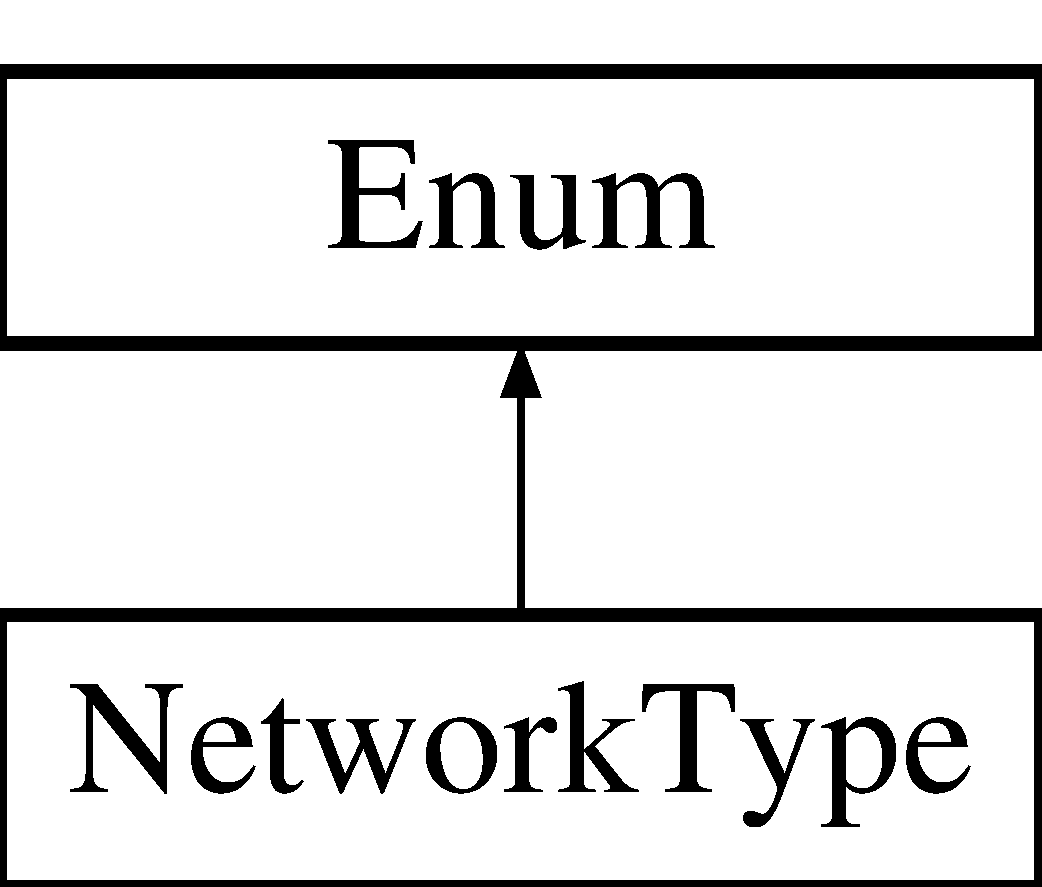
\includegraphics[height=2.000000cm]{class_mu_mo_t_1_1_network_type}
\end{center}
\end{figure}
\subsection*{Static Public Attributes}
\begin{DoxyCompactItemize}
\item 
\mbox{\Hypertarget{class_mu_mo_t_1_1_network_type_a6026c1d0088de63c8dbffa271c5cb8e4}\label{class_mu_mo_t_1_1_network_type_a6026c1d0088de63c8dbffa271c5cb8e4}} 
int {\bfseries F\+U\+L\+L\+Y\+\_\+\+C\+O\+N\+N\+E\+C\+T\+ED} = 0
\item 
\mbox{\Hypertarget{class_mu_mo_t_1_1_network_type_abfc09d249fa8a7e47ccae49424a21d61}\label{class_mu_mo_t_1_1_network_type_abfc09d249fa8a7e47ccae49424a21d61}} 
int {\bfseries E\+R\+S\+O\+S\+\_\+\+R\+E\+N\+YI} = 1
\item 
\mbox{\Hypertarget{class_mu_mo_t_1_1_network_type_a5684807d763efd4f800fe9a849cd962c}\label{class_mu_mo_t_1_1_network_type_a5684807d763efd4f800fe9a849cd962c}} 
int {\bfseries B\+A\+R\+A\+B\+A\+S\+I\+\_\+\+A\+L\+B\+E\+RT} = 2
\item 
\mbox{\Hypertarget{class_mu_mo_t_1_1_network_type_a03813c265f977cc034eb42fd3370bf3d}\label{class_mu_mo_t_1_1_network_type_a03813c265f977cc034eb42fd3370bf3d}} 
int {\bfseries S\+P\+A\+CE} = 3
\item 
\mbox{\Hypertarget{class_mu_mo_t_1_1_network_type_ad86080ad7b724db9fc31c1e654eba020}\label{class_mu_mo_t_1_1_network_type_ad86080ad7b724db9fc31c1e654eba020}} 
int {\bfseries D\+Y\+N\+A\+M\+IC} = 4
\end{DoxyCompactItemize}


The documentation for this class was generated from the following file\+:\begin{DoxyCompactItemize}
\item 
/\+Users/marshall/\+Google Drive/\+Home/\+Git/\+Mu\+Mo\+T/Mu\+Mo\+T.\+py\end{DoxyCompactItemize}

%--- End generated contents ---

% Index
\backmatter
\newpage
\phantomsection
\clearemptydoublepage
\addcontentsline{toc}{chapter}{Index}
\printindex

\end{document}
